\documentclass[oneside]{book}
\usepackage[a4paper, total={6in, 8in}]{geometry}
\usepackage[english]{babel}
\usepackage[utf8]{inputenc}
\usepackage[T1]{fontenc}
\usepackage{cancel}
\usepackage{amsmath}
\usepackage{amsfonts}
\usepackage{dsfont}
\usepackage{listings}
\usepackage{hyperref}
\usepackage{siunitx}
\usepackage{fancyhdr}
\usepackage{textcomp}
\usepackage{makecell}
\usepackage[font=small,labelfont=bf]{caption}
\usepackage{pdfpages}
\usepackage{multicol}
\usepackage[ruled,vlined]{algorithm2e}
\usepackage{soul}
\usepackage{mhchem}
\usepackage[toc, page]{appendix}
\usepackage{float}
\usepackage{wrapfig}
\usepackage{braket}
\usepackage{xcolor}
\usepackage{mathtools}
\usepackage{physics}
\usepackage{multirow}
\pagestyle{fancy}
\fancyhf{}
\lhead{\rightmark}
\cfoot{\leftmark}
\rfoot{\thepage}
\usepackage[export]{adjustbox}
\usepackage{wrapfig}
\usepackage{float}

\setcounter{secnumdepth}{5}

\lstset{
    frame=tb, % draw a frame at the top and bottom of the code block
    tabsize=4, % tab space width
    showstringspaces=false, % don't mark spaces in strings
    numbers=none, % display line numbers on the left
    commentstyle=\color{green}, % comment color
    keywordstyle=\color{red}, % keyword color
    stringstyle=\color{blue}, % string color
    breaklines=true,
    postbreak=\mbox{\textcolor{green}{$\hookrightarrow$}\space}
}

\renewcommand{\lstlistingname}{}% Listing -> Algorithm
\renewcommand{\lstlistlistingname}{Algoritmi}% List of Listings -> List of Algorithms


\renewcommand*{\listalgorithmcfname}{}
\renewcommand*{\algorithmcfname}{}
\renewcommand*{\algorithmautorefname}{}
\renewcommand{\thealgocf}{}
\newcommand{\mathcolorbox}[2]{\colorbox{#1}{$\displaystyle #2$}}


\title{\Huge\textbf{{Human genomics}}}

\author{
  Giacomo Fantoni \\
  \small telegram: \href{https://t.me/GiacomoFantoni}{@GiacomoFantoni} \\[3pt]
  Elisa Pettin\`a \\
  \small telegram: \href{https://t.me/elisapettina}{@elisapettina} \\[3pt]
  \small Github: \href{https://github.com/giacThePhantom/human-genomics}{https://github.com/giacThePhantom/human-genomics}\\
  Notes taken from lectures' recordings and:\\
  \small Github: \href{https://github.com/Maurizio319/HumanGenomics}{https://github.com/Maurizio319/HumanGenomics}
}


\begin{document}

  \maketitle
  \tableofcontents

  \part{Notes}
    \graphicspath{{chapters/notes/01/images/}}
\chapter{Introduction}

\section{Genetics and genomics}
Genetics is the study related to specific genes and their variants with a known effect on the phenotype.
Genomics is focused on the function and structure of the human genome, evolution and anything relating to the whole genome:

\begin{multicols}{2}
	\begin{itemize}
		\item Coding regions.
		\item Non-coding regions.
		\item Linear and non-linear structures.
		\item Cell physiology and pathology.
	\end{itemize}
\end{multicols}

	\subsection{Genetics}
	Genetics is the study of heredity, or how the characteristics of living organisms are transmitted from one generation to the next via DNA.
	It dates back to Augustinian friar and scientist Gregor Mendel.
	It involves the study of a specific and limited number of genes or their part that have a known function.

	\subsection{Genomics}
	Genomics is the study of the entirety of an organism's genes, the genome.
	Using high-performance computing and mathematics techniques known as bioinformatics, genomics researchers analyse enormous amounts of DNA-sequence data to find variations that affect health, disease or drug response.
	When dealing with the human genome that means searching through about $3$ billion units of DNA across $23000$ genes.

	\subsection{Differences between genetics and genomics}
	The main difference between genomics and genetics is that genetics scrutinizes the functioning and composition of the single gene, where genomics addressees all genes and their relationships in order to identify their combined influence on the growth and development of the organism.

	\subsection{The role of computational biology}
	Computational Biology encompasses a wide range of numerical methods to analyse and integrate large scale data towards the understanding of molecular, cellular and structural biology.
	Possible studies of computational biology are:

	\begin{multicols}{2}
		\begin{itemize}
			\item Semi-quantitative simulations of metabolic pathways.
			\item 3D protein-protein interaction.
			\item Characterization of 3D chromatic structure,
			\item Discovery and characterization of disease related variants.
		\end{itemize}
	\end{multicols}

	The main subjects involved are:

	\begin{multicols}{3}
		\begin{itemize}
			\item Biology.
			\item Genetics.
			\item Statistics.
			\item Calculus.
			\item Computer science.
			\item Bioinformatics.
		\end{itemize}
	\end{multicols}

	The focus of this work is on hot to mine raw data, mainly from sequencing, how to exploit it for quality control (QC) and hot to interpret the obtained results in the context of human diseases, especially in cancer.


\section{Basis of human genomics}
The genetic make-up is different in all human it is responsible for our diversity.
SNPs (single nucleotide polymorphisms) and CNVs (copy number variants) contribute to make us different.
The majority of the external phenotypes come from genetic variance that are inherited or, in minor measure, acquired.

	\subsection{Single nucleotide polymorphisms}
	Single nucleotide polymorphisms or SNPs are changes of one nucleotide in the sequence of a gene.
	They constitute $1\%$ of the difference between two unrelated individuals' genomes and they can be used as quality control assets.

	\subsection{Copy number variants}
	Copy number variants or CNVs are the differences in number of alleles for a gene present in one individual.
	They contribute much more than SNPs in the difference between unrelated individuals, but they're less known as inherited variants, as they are harder to quantify and detect.
	CNV are distinguished as gain-CNV (where the number of alleles is greater than two) and loss-CNV (where the number of alleles is $2$, $1$, or $0$).
	It is of note that if both parents have only one copy of a gene their child can have none.
	CNV span $\gg1\%$ difference between two unrelated individual genomes.

	\subsection{Inherited variants}
	Inherited variants can be characterized by penetrance and allele frequency.

	\begin{figure}[H]
		\centering
		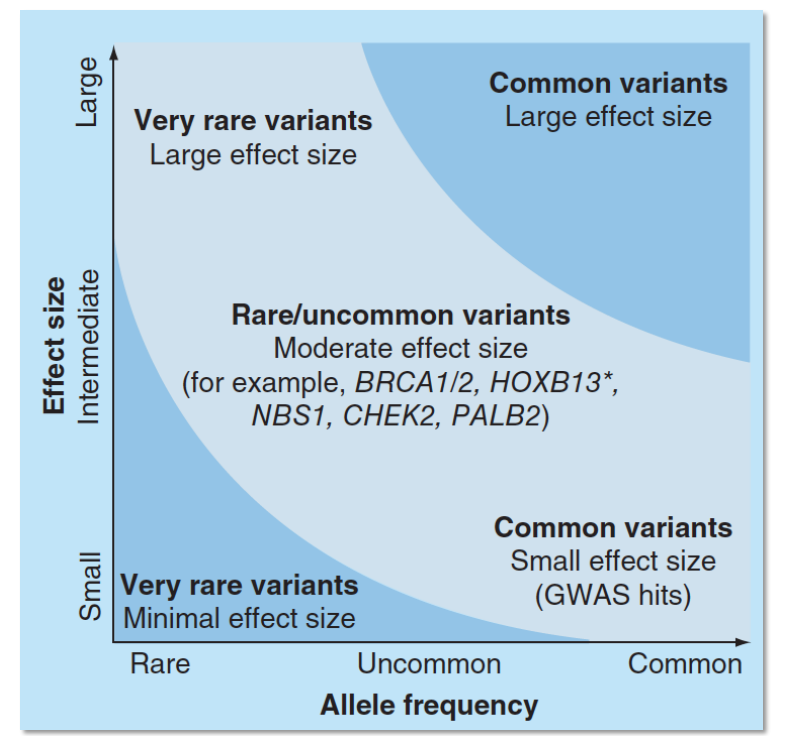
\includegraphics[width=0.5\textwidth]{relevance.png}
		\caption{R. Eeles, Future Sci. OA (2016) 2(1), FSO87. Review on prostate cancer.\\
			\textbf{Common SNPs}: $\frac{1}{4}$ of individual is homozygous for A1, $\frac{1}{4}$ is homozygous for A2, $\frac{1}{2}$ is heterozygous. The minor allele frequency is around 30-50\% with low penetrance.\\
			\textbf{Rare SNPs}: typically have very large size effect: if they are related to very specific traits they will have high penetrance. They constitute deleterious variants.}
		\label{fig:relevance}
	\end{figure}

		\subsubsection{Penetrance}
		Penetrance is the proportion of individuals carrying an allele (or genotype) that also expresses the trait (or phenotype) associated with it.

		\subsubsection{Allele frequency}
		Allele frequency is the ratio between the number of times the allele of interest is observed in a population over the total number of copies of all the alleles at that particular genetic locus in the population:

		$$AF = \frac{\# allele\ of\ interest}{\# copies\ of\ all\ the alleles\ at\ the\ genetic\ locus}$$

		Recent studies have shown that genetic variance contributes to predisposition to certain diseases.
		It is also emerging that rare pathogenic variants tend to have an high penetrance.
		This means that if a variant is pathogenic and rare, it's probable that all patients affected by the disease carry that particular mutation.
		This is represented by the top part of the diagram shown in figure \ref{fig:relevance}.
		On the other hand, common variants could be associated to predisposition or susceptibility to the disease with low penetrance.
		In the middle on the diagram well-known variants correlated to cancer are found.
		The majority of these have a moderate size effect: not everyone who has the variation develops the disease.

		\subsubsection{Differences in Genetic Make-Up, an example}
		One example of how the genetic make-up plays a role in disease is the ADME genes.
		ADME stands for \textit{Absorption, distribution, metabolism and elimination}.
		It is a set of genetic variants that is able to change the ability of the organism to react to certain compounds causing pharmacokinetic variability and influencing the patient's treatment response.
		Both common and rare variants are involved.
		Figure \ref{fig:adme} represent a subset of them.

		\begin{figure}[H]
			\centering
			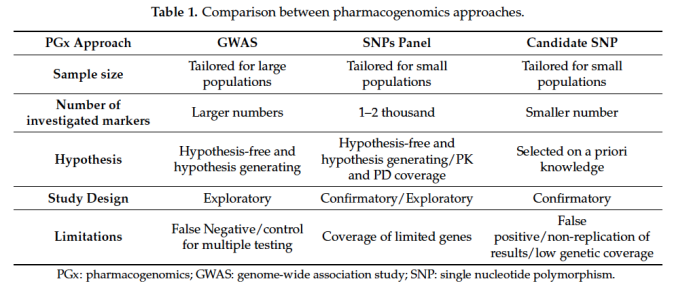
\includegraphics[width=0.7\textwidth]{ADME.png}
			\caption{From review: \textit{Pharmacogenomic Profiling of ADME Gene Variants: Current Challenges and Validation Perspectives}}
			\label{fig:adme}
		\end{figure}

		A therapeutic approach that considers these variations could be very useful in precision medicine.

	\subsection{Somatic Variants}
	Somatic variants are \textbf{not} inherited from parents and are not transmitted to offspring.
	Most of them, but not all, are harmless.
	They can also be present in only a subset of the cells in an individual.

		\subsubsection{Classification}
		Somatic variants can be classified as:

		\begin{multicols}{2}
			\begin{itemize}
				\item Single Nucleotide Variants (SNV).
					SNVs are a single point mutation restricted to a certain population of cells in an individual.
				\item Indels few nucleotides deletions.
				\item Rearrangements, like gene translocation, chromosome breakage and chromothripsis (which falls in the subcategory of chromosomal rearrangements).
				\item Somatic Copy Number Aberrations (SCNA).
			\end{itemize}
		\end{multicols}


		\subsubsection{Types of acquired DNA aberrations}

			\paragraph{Translocation}
			Translocation happens when a sequence is moved from one genetic locus to another.
			It can be:

			\begin{multicols}{2}
				\begin{itemize}
					\item Balanced: two sequences exchange locus and the overall quantity of DNA is maintained.
					\item Unbalanced: only one sequence move, generating an insertion.
				\end{itemize}
			\end{multicols}

			\paragraph{Inversion}
			Inversion happens when a sequence inverts its orientation.
			This aberration involves only one chromosome.
			The sequence of the inversion doesn't change, and the event will only be detected at its head and tail.

			\paragraph{Copy number changes}
			Copy number changes are events in which the quantity of DNA changes.
			They could involve one or more chromosomes.
			They can be:

			\begin{multicols}{2}
				\begin{itemize}
					\item Duplication: a sequence doubles its copy number.
					\item Deletion: a sequence is lost.
				\end{itemize}
			\end{multicols}

			\paragraph{Chromoplexy}
			Chromoplexy derives from the Greek \textit{pleko}, meaning to weave, or to braid.
			It describes a class of complex somatic DNA rearrangements whereby abundant DNA deletions and intra- and inter-chromosomal translocations that have originated in an interdependent way occur within a single cell cycle.

			\paragraph*{Chromothripsis}
			Chromothripsis derives from the Greek \textit{thripsis}, meaning shattering into pieces.
			It describes a clustered chromosomal rearrangement in confined genomic regions that results from a single catastrophic event, usually limited to one chromosome.

			\paragraph*{Kataegis}
			Kataegis derives from the Greek kataigis, meaning thunder.
			It describes a phenomenon that is characterized by large clusters of mutations (hypermutation) in the genome of cancer cells.
			An APOBEC family enzyme might be responsible for the kataegis process.

\section{Experimental techniques to detect variants/aberrations}

	\subsection{Karyotyping}
	Karyotyping is the process of pairing and ordering all the chromosome of an organism, providing a genome-wide snapshot of an individual's chromosomes.
	This experiment was used to try and detect genomic aberration, but it proved inadequate because its resolution wasn't enough.
	In particular it missed all sequence specific variants, breakpoints that could not be detected until the development of NGS.

	\subsection{Sequence capture for cancer genomics}
	In the paper summarized in \ref{ch:Meyerson} it is described a typical sequence capture for cancer genomics.

		\subsubsection{Reference}
		After sequencing there is a need to align the reads to a reference genome.
		This is especially needed when studying somatic changes.
		The best reference for this king of studies is the individual's own genome, usually retrieved from white blood samples.
		Both cancer and normal DNA can be aligned to detect if an aberration is cancer specific or is present in both normal and cancer DNA.
		The \textbf{match normal} tool is used to distinguish SNV from rare SNPs, somatic and germline indels, but also to make sure that copy number variations are somatic.
		Baits are nowadays used in the sequencing step, in order to sequence only the exome or specific part of the genome, as to make the sequencing process more cheap.

		\subsubsection{Deepness}
		Another fundamental parameter in sequencing is the deepness.
		A more deep sequencing is needed to find subclonal event that could increase cancers' fitness, like the ability to escape the immune system.
		It is necessary because not all cells present all the mutations characterizing the subclonal event and because the purity of a tumour sample is not always optimal.


		\subsubsection{Single End (SE) and Paired End (PE) reads} \label{SE_PE}

			\paragraph{Single end sequencing}
			Single-read sequencing involves sequencing DNA from only one end.
			This solution delivers large volumes of high-quality data, rapidly and economically.

			\paragraph{Paired end sequencing}
			Paired-end sequencing allow to sequence both ends of a fragment and generate high-quality alignable data.
			It facilitates the detection of genomic rearrangements and repetitive sequence elements, as well as gene fusions and novel transcripts while providing double the coverage as a single-end protocol.
			It gives important information of the relative position of a molecule with respect to the reference, and is a necessary choice when structural aberration need to be assessed.
			This protocol is however twice as expensive as the single-end one.

			\paragraph{Ability of paired end sequencing to detect genomic aberrations}
			Figure \ref{fig:igv} gives a nice graphical overview of genomic aberrations detectable by NGS, especially using PE sequencing.
			In particular the traslocation breakpoint in figure \ref{fig:igv} would not be detectable without paired end sequencing.
			The most important parameter when studying deletions and insertion is to have enough coverage to perform significant downstream analysis, besides structural informations.

			\begin{figure}[H]
					\centering
					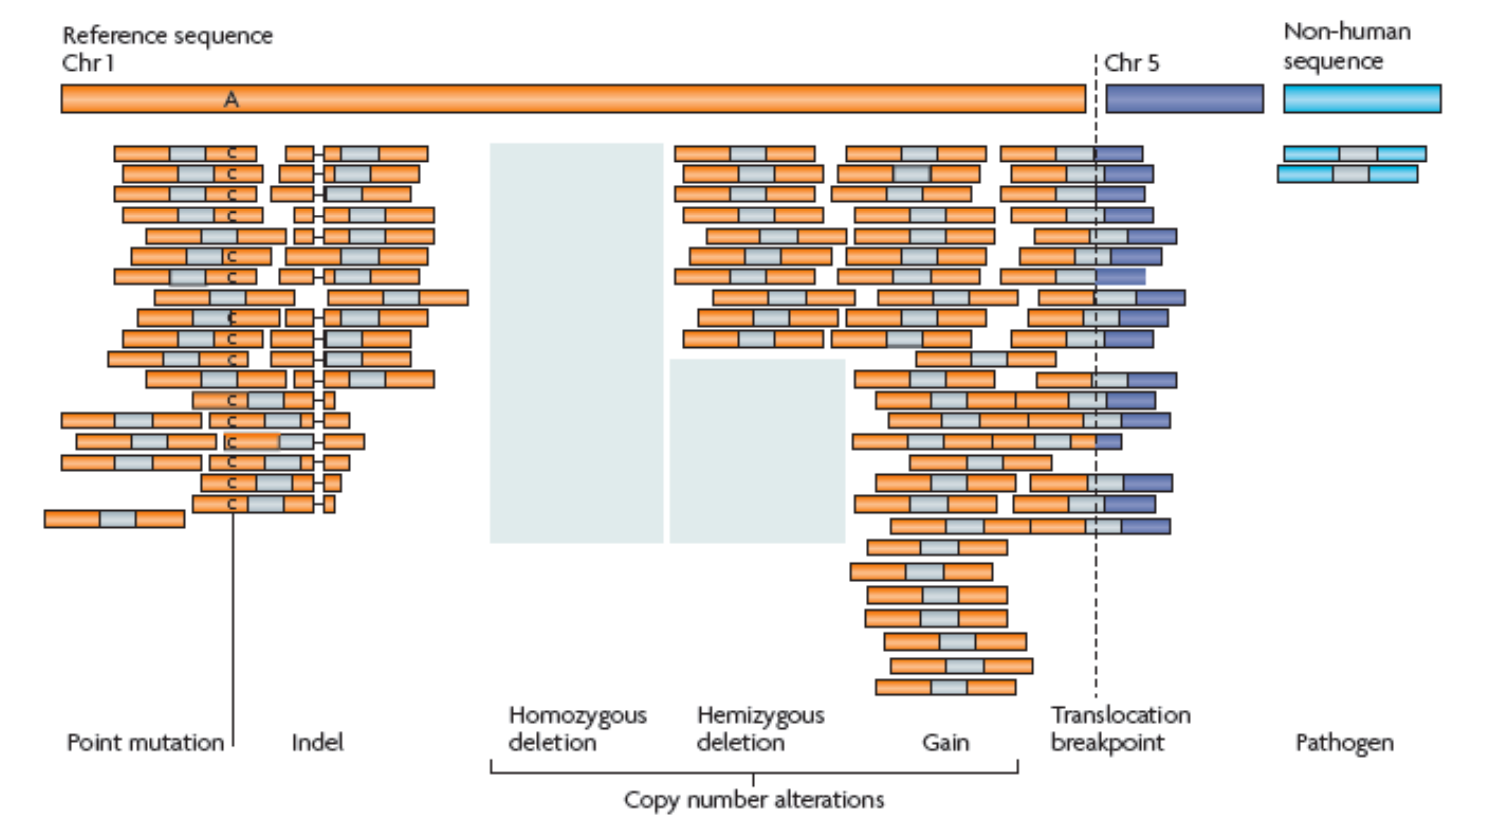
\includegraphics[width=0.7\textwidth]{igv.png}
					\caption{\textit{Advances in understanding cancer genomes through second-generation sequencing}, Meyerson et al., Nature Reviews Genetics 2010}
					\label{fig:igv}
			\end{figure}

    \graphicspath{{chapters/notes/02/images}}
\chapter{Coverage}
\section{Local Coverage and Allelic Fraction}
Two key concepts needed when performing genomics analysis are the \textbf{local coverage} and \textbf{allelic fraction}.

	\paragraph*{Local coverage (cov)}
		The local coverage (cov) at position (base) $i$ is the number of reads that span $p_i$.
	\paragraph*{Allelic fraction (AF)}
		The allelic fraction (AF) at position $i$ is the proportion of reads that supports 			the reference base in $p_i$, and vice versa.

The Lander-Waterman equation to compute NGS coverage is:
\begin{equation}
C = \frac{L * N}{G}
\end{equation}
Where C is the coverage, G is the haploid human genome length, L the read length and N the number of mapped reads.

\subsection{Mapping in NGS}
The number of mapped reads is always lower than expected. Errors, or major translocation will impair a good mapping of the reads. \\
There's a difference between physical and sequence coverage. Physical coverage is always higher, and it changes based on which protocol (PE or SE) is chosen for the assay.
To put it simply, when calculating the sequence coverage we only take into account the actual ends, while when calculating the physical coverage we also account for the consequence part of the PE protocol. In figure \ref{fig:seq_phys} a  schematic representation of this problem is displayed.
\begin{figure}[H]
    \centering
    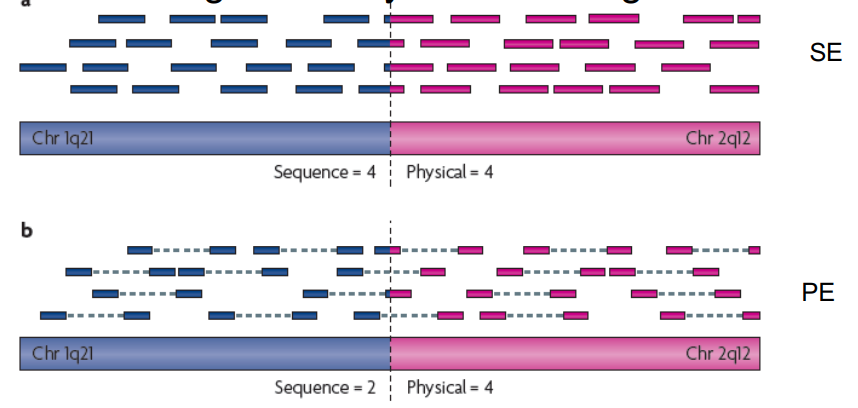
\includegraphics[width=0.5\textwidth]{seq_phys.png}
    \caption{Schematic difference between sequence (on the left) and physical coverage (on the right). From Meyerson et al., Nature Reviews Genetics 2010}
    \label{fig:seq_phys}
\end{figure}

Formal definitions of sequence and physical coverage are:

\paragraph*{Sequence coverage:}
	Sequence coverage is the amount of oversampling (how many times a base is sequenced); to detect nucleotide alterations with high sensitivity, the 3 billion bases of the human genome have typically been ‘covered’ with at least 30-fold (30X) on average, meaning 90 billion bases of sequence data per sample.
	\paragraph*{Physical coverage:}
		the expected distance between the paired reads is used to uniquely place the reads on the genome; unexpected read pairs are used to detect structural anomalies.



\section{Tuning the intended coverage of a NGS assay}
In some experiments setups there's the need to carefully control the amount of intended coverage. \\
If we are looking for SNPs only, which by definition are present in all of the cells, we only need enough redundancy (local coverage) to detect them and distinguish the reference base and the alternative base (in case of an heterozygous SNP we will ideally find half of the reads supporting the reference and half supporting the alternative). Indeed for SNPs we do not need more than 10-15 X coverage.
\\
However, if the sample comes from a tumor or hematopoietic events, we need to look for subclonal events. Subclonal events are not harbored by all of the cells but only by a fraction of them. If we expect 1/4 of the cells harboring the mutation, we need to increase the coverage. \\
The same reasoning goes for any monozygous mutation and any low abundant events, and for  transcripts expressed at very low level (RNA-seq) and weak binding in ChIP-Seq.

\subsection{Example on the importance of coverage}
Here are represented 10 genes relevant for cancer. Each bar represents the average local coverage at 30 bp.
\begin{figure}[H]
    \centering
    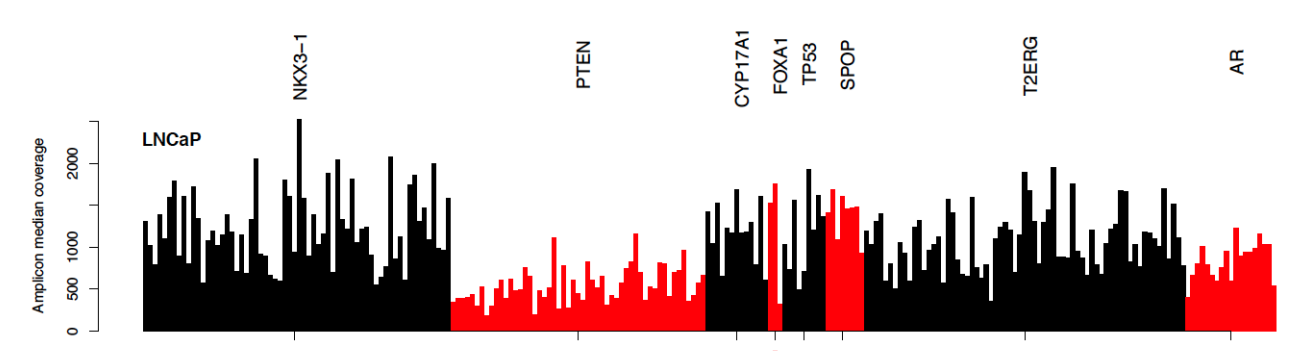
\includegraphics[width=0.5\textwidth]{local_coverage.png}
    \caption{Example of local coverage. On the x axis genomic location (on top e ery gene) and the bars is the number of amplicons. }
    \label{fig:local}
\end{figure}

In figure \ref{fig:local} a barplot can be observed, representing the local coverage (y axis) in the gene locations (x axis). The \textit{cov} is on average about 600x and it's "wavy", not evenly distributed (very typical). However, if one would do an average of the coverage for each gene, they would discover that one gene is abundantly underrepresented: PTEN.\\
What's happening on PTEN base on plot \ref{fig:local}? Probably, the most accurate guess is a deletion. But of which kind? For sure not a homozygous deletion, since we would not be able to see any signal in the plot. From this data however we cannot say whether this is a monoallelic or biallelic deletion. \\
Note that this (and the following \ref{fig:local2}) plot is the actual way sequencing data is shown, while the figure presented in \ref{SE_PE} was a schematic representation.

\begin{figure}[H]
    \centering
    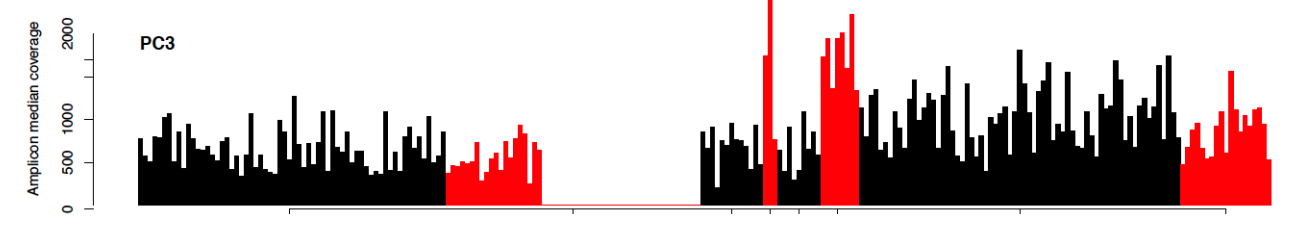
\includegraphics[width=0.5\textwidth]{local_coverage1.png}
    \caption{Example 2 of local coverage. The  cell line is different (PC3 instead of LNCaP). }
    \label{fig:local1}
\end{figure}

However, in the plot \ref{fig:local1}, from a different cell line, we can see a clear monoallelic deletion and a partial biallelic deletion of PTEN.\\

\begin{figure}[H]
    \centering
    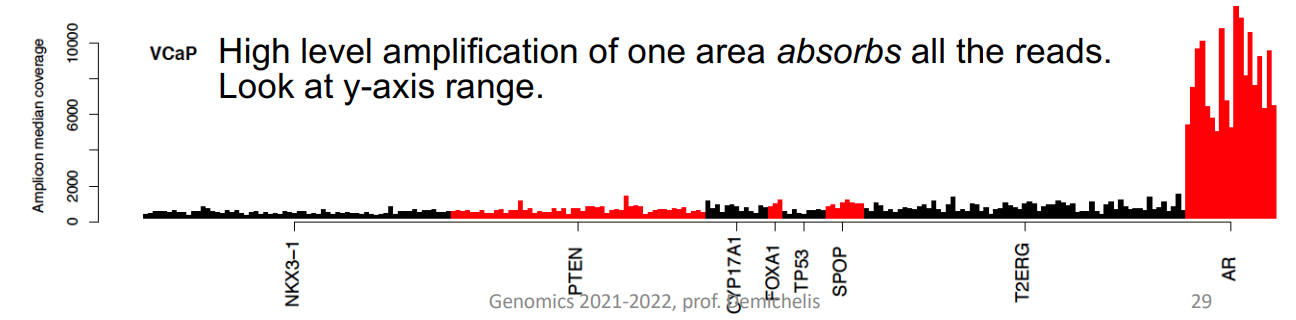
\includegraphics[width=0.5\textwidth]{local_coverage2.png}
    \caption{Example 3 of local coverage. The  cell line is different (VCaP). The massive amplification of the AR region is typicall in advanced prostate cancer.}
    \label{fig:local2}
\end{figure}

In figure \ref{fig:local2} we can see a massive amplification of the antigen receptor. Probably it was a mistake in the assay: amplification on the AR does not allow the analysis/discovery of other copy number variations because all of the reads will go to the AR site. \\
These were amplicon-based approaches.
With NGS instead, It is easy to increase the experimental coverage (i.e. the sequence depth) at later point in time.
Provided our original sample/library is still available, we can perform another run of sequencing and then combine the output from different runs.
Note that this isn’t possible with array-based technologies.\\
However, there are some limiting factors of NGS DNA-seq experiments.
Problems with repeated regions, but also not knowing the linearity of the genome.
If the sequencing is done with longer reads we could tackle the problem by having longer molecules to work with, but there are more errors in the reads.

\subsection{Databases}
Two very known databases for NGS analysis are:
\begin{itemize}
\item \textbf{Genome Reference Consortium}: assemble a reference genome reflecting the most common sequences in population at each position while tracking information on polymorphisms.
\item \textbf{USCS Genome Browser}: select a reference genome and query all known features.
\end{itemize}

\section{Interpreting Pair Orientations}
We will now look at some aberrations' discoveries performed using IGV.\\
In IGV, each vertical bar corresponds to a read.
If there is a colored sign, there is a polymorphism or difference with respect to a reference.
The browser also gives info about the quality of the read and bases (and others from the BAM file).\\
While using a paired-end protocol, we can study inversions, duplications and translocations. A useful legend to navigate the subsequent example is reported in the list below.
\begin{itemize}
\item \textbf{LR} ($\rightarrow \, \, \, \leftarrow$): Illumina (convention), the reads are left and right of the unsequenced part of the sequenced DNA fragment when aligned back to the reference genome.
\item \textbf{LL}, \textbf{RR}: implies inversion in sequenced DNA with respect to reference.
\item \textbf{RL}: implies duplication or translocation with respect to reference.

\end{itemize}

\subsection{Inversion}
To detect major aberration, like inversions, we need reads that span the breakpoint (either long reads, or, better, PE reads). \\
What's happening exactly at the breakpoint in figure \ref{fig:inversion}? What's the coverage when looking at the data?  When we map them on the reference, we see that the direction is LL and RR, meaning that there is an inversion.
%The sequence that we have in the molecule does not exist there and therefore that sequence doe not exist in two copies in the molecule.
We can also spot a drop in the local coverage.
In the target molecule, either it does not exist or exist only in one allele and not the other one. \\
When interpreting structural variance, we need not to care only about end-orientation, but also coverage at the exact break point, which is due to the fact that the inverted breakpoint sequence does not exist in the reference genome.


%\begin{figure}[htbp!]
    %\centering
    %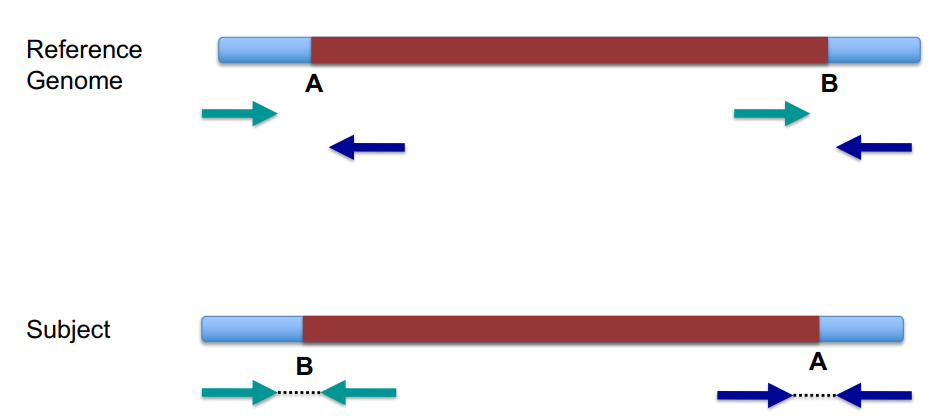
\includegraphics[width=0.5\textwidth]{inversion.png}
   % \caption{Inversion discovering exploiting PE reads.}
   % \label{fig:inversion}
%\end{figure}

\begin{figure}[H]
\begin{tabular}{cc}
  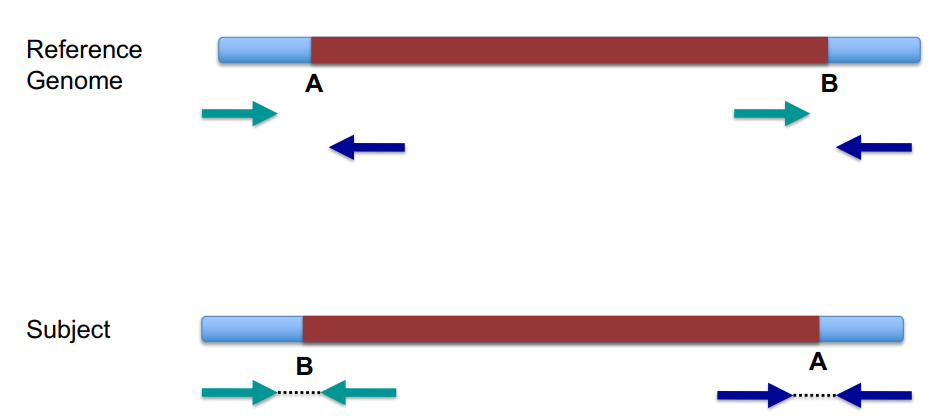
\includegraphics[width=0.5\textwidth]{inversion.png} &   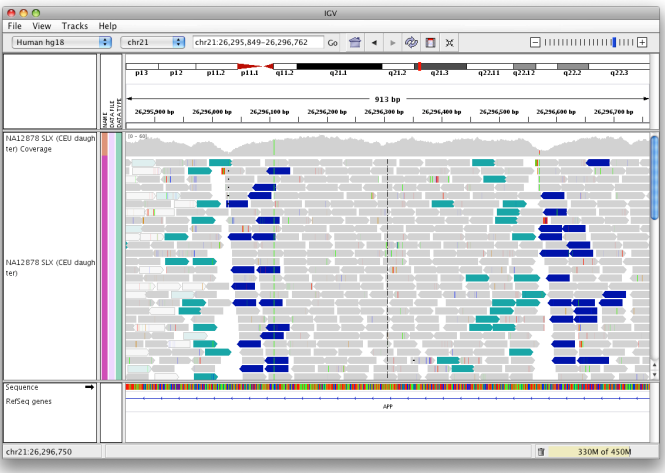
\includegraphics[width=0.5\textwidth]{inversion_igv.png} \\
(a) Schematic & (b) IGV view \\[6pt]

\end{tabular}
\caption{Inversion discovering exploiting PE reads.}
\label{fig:inversion}
\end{figure}



\subsection{Tandem duplication}
Notice how in the tandem duplication (figure \ref{fig:tandem}) all the reads that do not cover the junction point align perfectly to the reference.
The coverage will be 3/2 of the expected value, proportional to the extra copy. B junction and A junction will not have modifications. If we had a read mapping BA, we would observe a partial alignment at B on the reference.
We observe no drop of coverage because the sequences also exist in the reference. \\


\begin{figure}[H]
\begin{tabular}{cc}
  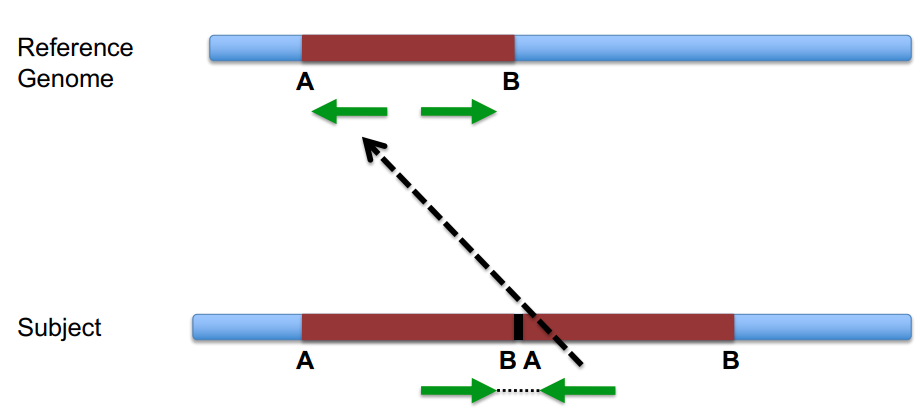
\includegraphics[width=0.5\textwidth]{tandem.png} &   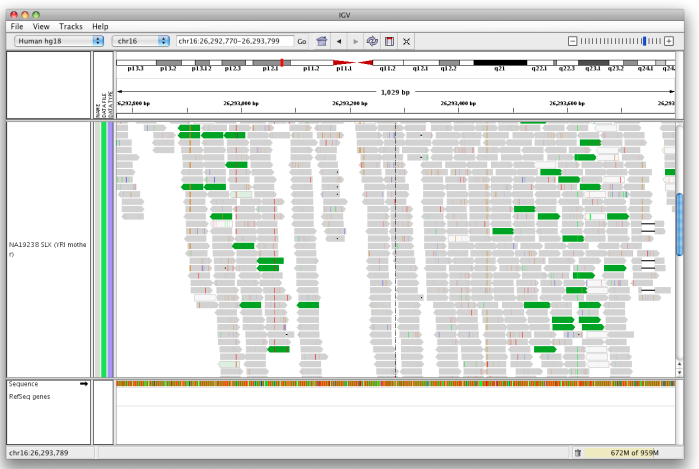
\includegraphics[width=0.5\textwidth]{tandem_igv.png} \\
(a) Schematic & (b) IGV view \\[6pt]
\end{tabular}
\caption{Tandem duplication discovering exploiting PE reads.}
\label{fig:tandem}
\end{figure}

\subsection{Inverted duplication}
For the inverted duplication, in figure \ref{fig:inverted}, we expect double coverage in the duplicated site in the reference genome. \\
Both A and B on the first segment on the subject are LR oriented, and the same occurs in the reference genome.
When we add the second fragment the same holds, but direction will be LL and RR and the insert size will be significantly longer. In particular, we can notice that we have an overlapping of left and right reads on the reference. Furthermore, the coverage depth will highly increase due to the presence of multiple reads on the reference genome.

\begin{figure}[H]
\begin{tabular}{cc}
  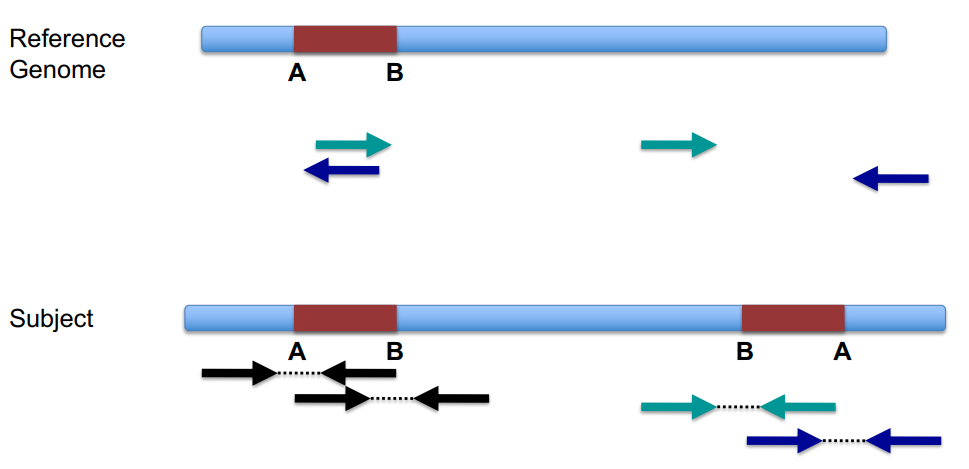
\includegraphics[width=0.5\textwidth]{inverted.png} &   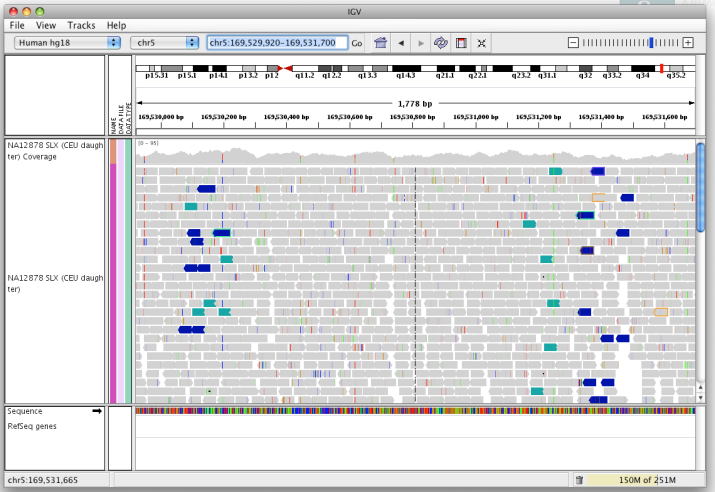
\includegraphics[width=0.5\textwidth]{inverted_igv.png} \\
(a) Schematic & (b) IGV view \\[6pt]
\end{tabular}
\caption{Inverted duplication discovering exploiting PE reads.}
\label{fig:inverted}
\end{figure}

What if we have a deletion? How can you guess the size of it? We can look at the coverage or observed distance between the reads, which gives clean indication of the size of the deletion. For tiny deletions, smaller than the length of the read, we use the sequence within the reads and in this way discovering indels.

\section{Summary}
Summarizing, the elements to consider are:
 \begin{itemize}
 \item Pair ends relative orientation;
 \item Insert size length;
\item Coverage within the aberrant region;
\item Coverage outside of the aberrant region (flanking genomic segments);
\item Coverage at the breakpoints.
 \end{itemize}

    \graphicspath{{chapters/notes/03/images}}
\chapter{Genetic Fingerprinting}

\section{Introduction}
Genetic fingerprinting is a technique used to investigate some characteristics of a genome, typically a pattern of variable elements, like SNPs or minisatellites, in order to uniquely characterize a genome.
It can be used to compare a genome with a reference sample or to compare different genomes between each other in order to determine their diversity or analogy.

	\subsection{Fields of interest}
	DNA fingerprinting is used in different fields, like:

	\begin{multicols}{2}
	\begin{itemize}
			\item In forensics for identification purposes.
			\item In lineage related tests, for cells or humans like paternity or hereditary tests.
			\item For the certification of the origin of cells used in the laboratory, to make sure that the cells are the right ones and that there are no major genetic drifts.
				It is necessary when using certain cell lines in an experiment for publishing purposes.
			\item To identify and remove samples that would skew the data.
				For example members of the same family when performing a GWAS study on a certain geographic area.
		\end{itemize}
	\end{multicols}

	\subsection{Variants used for genetic testing}
	Different variants can be used for genetic fingerprinting, such as Single Nucleotide Polymorphisms (SNPs) or inherited Copy Number Variations (CNVs).
	In the past, before sequencing and SNPs array, short tandem repeats were commonly used for genetic fingerprint.

		\subsubsection{CNVs}
		CNVs are a phenomenon in which sections of the genome are repeated or deleted, changing the number of times those regions appear in the genome.
		The most amenable type of inherited CNVs for genetic fingerprinting are the loss-CNVs.
		For a loss CNV in the population the copy number can vary between $2$ and $0$.
		In particular if both parents are heterozygous for a particular CNV their offspring could have an homozygous deletion.
		If instead both parents have $2$ copies at a site that is polymorphic in the population, all of their offspring will have a copy number of $2$.
		Gain-CNVs are difficult to analyse for this tests because when combining multiple copies the origin of a single copy number cannot be traced to a parent and so they cannot be used for genetic fingerprinting.

		\subsubsection{SNPs}
		SNPs are substitutions of a single nucleotide at a specific position in the genome.
		They are the most amenable type of variation as they are simple, abundant in the genome and easy to detect in sequencing data even with low coverage.
		For these reasons the focus of this work will be on SNP-based genetic tests.


\section{SNPs features}

	\subsection{Hardy-Weinberg equilibrium}
	One property of SNPs which has to be taken into account when using them for genetic testing is the Hardy-Weinberg equilibrium.
	In population genetics, the Hardy-Weinberg equilibrium states that allele and genotype frequencies in a population will remain constant from generation to generation under neutral selection, so in the absence of other evolutionary influences, like:

	\begin{multicols}{4}
		\begin{itemize}
			\item Genetic drift.
			\item Mate choice.
			\item Sexual selection.
			\item Mutation.
		\end{itemize}
	\end{multicols}

	In the simplest case of a single locus with two alleles denoted $A$ and $a$ with frequencies $f(A) = p$ and $f(a) = q$ in a population the expected genotype frequencies under random mating are:

	\begin{multicols}{3}
		\begin{itemize}
			\item $f(AA) = p^{2}$ for $AA$ homozygotes.
			\item $f(aa) = q^{2}$ for $aa$ homozygotes.
			\item $f(Aa) = 2pq$ for $Aa$ heterozygotes.
		\end{itemize}
	\end{multicols}

	In the absence of selection, allele frequencies $p$ and $q$ are constant between generations, reaching an equilibrium.
	The general equation that the allele frequencies need to fit in to be considered in equilibrium is:

	$$( P + Q )^2 = 1 \qquad\land\qquad P^2 + 2PQ + Q^2 = 1$$

	SNPs that respect this equilibrium are the most studied and thus the most informative.

	\subsection{Minor allele frequency}
	Minor allele frequency is the frequency at which the second most common allele occurs in a given population.
	When performing genetic fingerprinting, the aim is to maximize the probability to have different genotypes in unrelated individuals.
	For this reason, the more advantageous SNPs will be the ones in which the allelic frequency of the variants is the highest possible.
	Highest variability in the population allows to distinguish better more individuals.

		\subsubsection{Optimal MAF values for genetic fingerprinting}
		Number-wise, a frequency of $\frac{1}{3}$ for each SNP would maximize the variability in a population, but those SNPs wouldn't be in Hardy-Weinberg equilibrium generating possible missed calls.
		Therefore, the optimal SNPs to detect individuals’ differences and similarities are those with genotype frequencies:

		\begin{multicols}{3}
			\begin{itemize}
				\item $P_{AA} = 0.25$.
				\item $P_{BB} = 0.25$.
				\item $P_{AB} = 0.5$.
			\end{itemize}
		\end{multicols}

		So the best SNPs will be those with $MAF = 0.5$.

	\subsection{Haplotype blocks}
	Another important feature to consider for SNPs selection are Haplotype blocks.
	They are blocks along the genome that tend to be inherited together as segments.
	In these regions there is little evidence for historical recombination and only a few common haplotypes are observed.
	Because of this to perform genetic fingerprinting it is enough to consider only a SNPs per haplotype block because the other won't bring additional information.

		\subsubsection{Linkage disequilibrium}
		SNPs in the same HB are said to be in Linkage Disequilibrium (LD).
		Linkage disequilibrium is a measure of the non-random associations between alleles or polymorphisms at different loci.
		A higher LD indicates SNPs with a stronger tendency to co-segregate.
		Haplotype Blocks are therefore commonly represented with linkage disequilibrium plots like the one in figure \ref{fig:linkage}.
		In these plots, SNPs are represented in a way that does not respect the genomic distance, but the order along the genome or the position of each SNP relative the others.

		\begin{figure}[H]
			\centering
			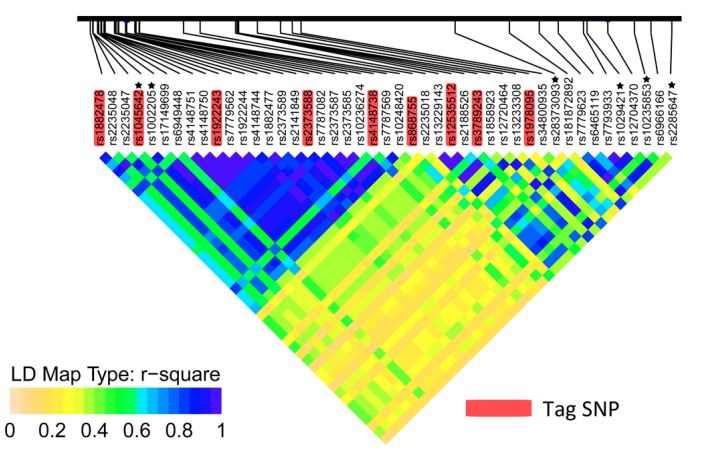
\includegraphics[width=0.7\textwidth]{linkage.png}
			\caption{\label{fig:linkage}LD plot of SNPs with top-ranked bayes factors in CHB (Han Chinese in Beijing) of 1000 Genome Phase I. The colors indicate the strength of pairwise LD according to $r2$ metrics. The SNPs marked with asterisks represent independent strong associations. Tag SNPs are here shadowed in pink.}
		\end{figure}

		The colors indicate the strength of pairwise linkage disequilibrium (LD) according to the $r2$ metrics, the proportion of the variation in the dependent variable that is predictable from the independent ones.
		In fact, not all of the SNPs are informative to distinguish between individuals.

		\subsubsection{Tag SNPs}
		In figure \ref{fig:linkage} tag SNPs are shadowed in pink.
		A tag SNP is representative of a region with high linkage disequilibrium and represents a group of SNPs or haplotype.
		This tag SNPs are the ones that will be included in a genetic fingerprinting test.

	\subsection{Other SNP features}
	Other SNP features to take into consideration when performing a genetic fingerprinting test are:

	\begin{multicols}{2}
		\begin{itemize}
			\item Exclude chromosomal locations which undergo frequent somatic aberrations.
				For example areas commonly deleted in tumour will produce LOH but probably also no calls, since there is no DNA to be sequenced.
			\item Choose SNPs equally spread all around the genome so to represent it all.
			\item Select only autosomal SNPs.
			\item Select SNPs in exons, so to have signal even from a non-DNA assay.
			\item Exclude or include disease or drug response associated loci.
			\item Include or exclude loci with significantly different MAF in different ethnicity.
				Including them allow to perform a lineage test in the same assay.
		\end{itemize}
	\end{multicols}

	\subsection{Number of SNPs to select when performing a genetic test}
	The number of SNPs needed to run a genetic fingerprinting test must be assessed.
	This number should be allow the measure of the test to differentiate unrelated individuals.
	When choosing this number experimental and biological mismatches must be taken into account, weighted based on their likelihood.
	When choosing the number of SNP all the possible mismatches must be taken into account, increasing it to allow to identify individuals.

		\subsubsection{Experimental mismatches - Genotype call error rate}
		During sequencing errors can occur, resulting in no data available for some loci, that if they include SNPs of interest will cause a loss of a call for that SNP.
		These experimental mismatches are related to the error rate of the technology used and because of this they are platform dependent.

			\paragraph{An example on the effect of experimental mismatches}

			\begin{figure}[H]
				\centering
				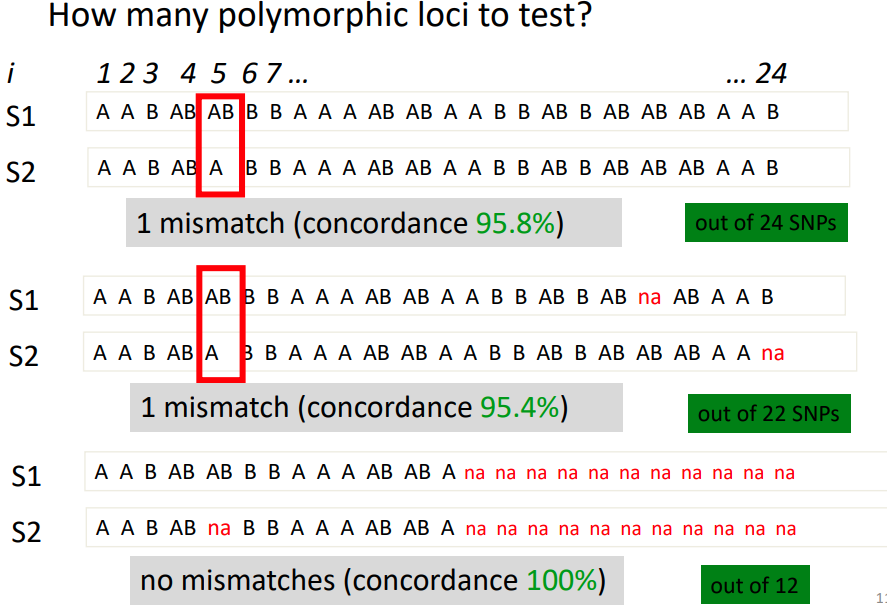
\includegraphics[width=0.6\textwidth]{SNP.PNG}
				\caption{Effect of the error rate on concordance}
				\label{fig:SNP}
			\end{figure}

			In each example in figure \ref{fig:SNP} two sample for which $24$ SNPs are called are analysed.
			To determine the difference of the two samples genotype for each position is considered and mismatches counted.
			In the figure:

			\begin{multicols}{3}
				\begin{itemize}
					\item 'A' stands for homozygous for the reference.
					\item 'B' stands for homozygous for the alternative.
					\item 'AB' stands for heterozygous.
				\end{itemize}
			\end{multicols}

			Analysing now SNPs calls:

			\begin{multicols}{2}
				\begin{itemize}
					\item In the first test over the $24$ loci, there is only one mismatch.
						The level of concordance is $95.8\%$.
						So the individual are highly related or the DNA come from the same sample.
					\item In the second test there is only one mismatch but there are position without a call.
						Therefore the concordance is measured out of $22$ SNPs and is equal $95.4\%$.
					\item In the third test there are a lot of missing calls, so only $12$ SNPs are available and concordance is $100\%$.
				\end{itemize}
			\end{multicols}

			This different level of concordance is due to missing calls in the second and third test.
			The first is the most accurate as it considers the greater number of SNPs between the three, providing the most reliable information.

		\subsubsection{Biological mismatches}
		In the context of disease samples and tumours, many somatic events can happen, like deletions, gains of copies or homozygous deletions.
		This events can change the genetic make-up of a person and have to be taken into account when performing a genetic test.

			\paragraph{Loss of Heterozygosity (LOH)}
			LOH is an event that results in the loss of one parental copy of a region which results in the genome having just one copy of that region.
			If that region contained a heterozygous locus, there will be loss of heterozygosity.
			Its probability of arising is:

			$$P(AB, A) = P(AB)\cdot P(A|AB)$$

			\paragraph{Gain Of Heterozygosity (GOH)}
			GOH is due to a mutation in a site.
			It is polymorphic through inheritance.
			These types of events are pretty rare and their probability of arising is:

			$$P(A,AB) = P(A) \cdot P(AB | A)$$

			\paragraph{Double Mutation (DM)}
			Double mutations are event when a mutation occurs on an already mutated event.
			They are very rare and their probability of arising is:

			$$P(A,B) = P(A) \cdot P(B | A)$$

			\paragraph{Modelling biological mismatches}
			Biological mismatches can be modelled in an assay in a data driven way, assessing the error rate for genotyping for some specific SNPs or running specific tests.
			The resolution for the errors of these mismatches can be patient-wide or tissue-specific.


	\subsection{Project regarding SNPs}
	Some useful projects developed over the years are:

	\begin{multicols}{2}
		\begin{itemize}
			\item dbSNPs.
			\item HapMap3.
		\end{itemize}
	\end{multicols}

		\subsubsection{dbSNPs}
		dbSNPs is a database of small scale nucleotide variants.
		It includes both common and rare single base nucleotide variation (SNV), short ($\leq$ 50bp) deletion/insertion polymorphisms, and other classes of small genetic variations.
		It can be found on \url{https://www.ncbi.nlm.nih.gov/snp/}.

		\subsubsection{HapMap3}
		HapMap3 is the third phase of the HapMap project whose aim is to develop a haplotype map of the human genome to describe the common patterns of human genetic variation in order to allows researchers to find genes and genetic variations that affect health, disease and individual responses to medications and environmental factors.
		The HapMap is a catalog of common genetic variants that occur in human beings.
		It describes what these variants are, where they occur in our DNA, and how they are distributed among people within populations and among populations in different parts of the world.
		It can be found on \url{https://www.sanger.ac.uk/resources/downloads/human/hapmap3.html}

\section{Genetic distance}
Having defined the number of SNPs to use, with maximum MAF and other amenable characteristics, the genetic test should provide a measure of the genetic distance between individuals associated with a probability of the measure to be correct.

	\subsection{Measuring distance}
	As a simple measure, the number of loci where two samples show different genotype can be counted and normalized on the total number of queried loci, defining a certain level of discordance.
	The output value will be the genetic distance between the two samples given the selected loci, which will be proportional to the number of discordant calls.
	In figure \ref{fig:Distance} a typical graph used to measure the genetic distance using SNP-based genetic testing is depicted.
	$4$ samples with a set of $5$ SNPs for each one are analysed.
	The distance is measured among all possible pairs, whose indexes are reported on the x-axis.

	\begin{figure}[H]
		\centering
		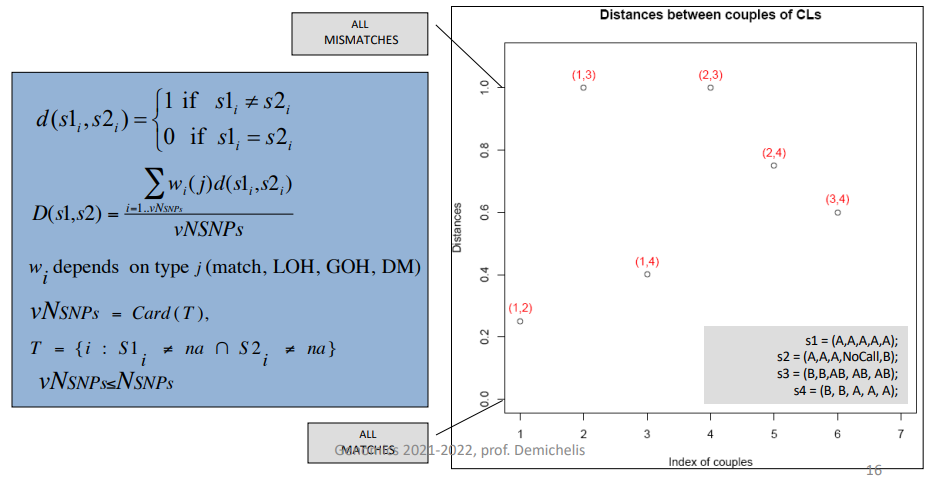
\includegraphics[width=0.7\textwidth]{loci.PNG}
		\caption{Genetic Distance graph with 4 samples. On the y axis the genotype distance is represented, varying from $0$, total concordance to $1$ total discordance. On the x-axis all possible pairs in the dataset are included.}
		\label{fig:Distance}
	\end{figure}

	In particular in figure \ref{fig:Distance}:

	\begin{multicols}{2}
		\begin{itemize}
			\item $s1$ and $s2$ have $3$ equal calls, one locus without call and a mismatch.
				The genetic distance is $0.25$.
			\item Samples $s1$ and $s3$ have $5$ mismatches out of $5$ SNPs, so the genetic distance is $1$.
		\end{itemize}
	\end{multicols}

	The equation in \ref{fig:Distance} is the one used to compute genetic distance.
	The weight $w_i$ can be used to associate different importance to different mismatches.
	The distance is normalized by the total number of SNPs for which there are available calls $vNSNPs$, such that $vNSPNs\le NSNPs$, the total number of SNPs considered in the test.

		\subsubsection{Expected distance}

		\begin{figure}[H]
			\centering
			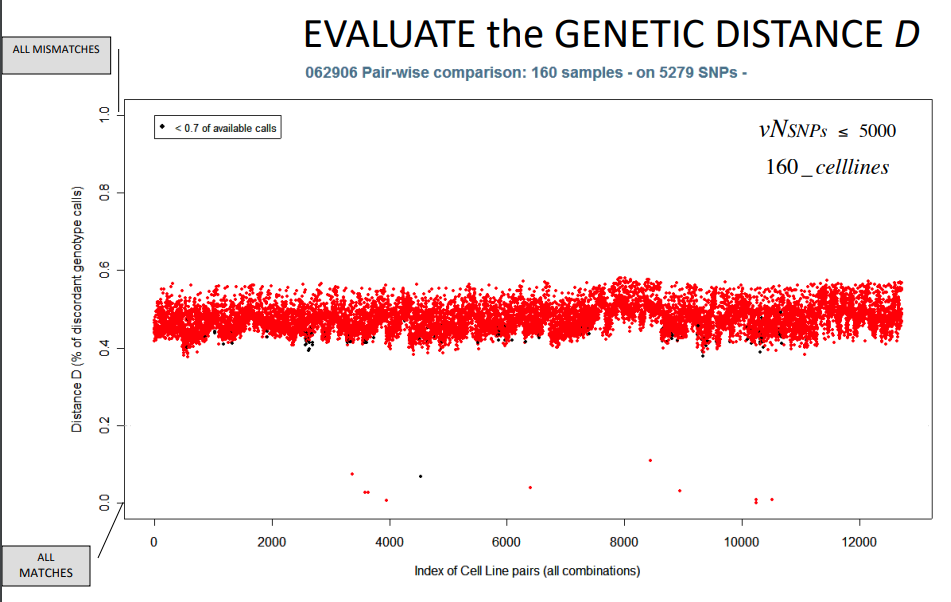
\includegraphics[width=0.7\textwidth]{loci2.PNG}
			\caption{Genetic Distance graph with 160 samples}
			\label{fig:Distance2}
		\end{figure}

		Figure \ref{fig:Distance2} shows the distance, measured by genetic fingerprinting, of a collection of 160 samples of cell lines.
		There are $\frac{160\cdot159}{2}$ possible pairs.
		Applying the distance measure to a larger collection of samples an average distance among all possible pairs is expected.
		This, for different samples will be close to $1$, never reaching it due to genetic variance and errors.
		In this case the average distance is around $0.5$, since by chances some samples share some genotypes.
		Some pairs have a low distance: this is due to a mislabelling to the cell lines used: some believed to be two different cell lines were in fact the same one.

		\subsubsection{Identifying a sample origin from RAP samples}

		\begin{figure}[H]
			\centering
			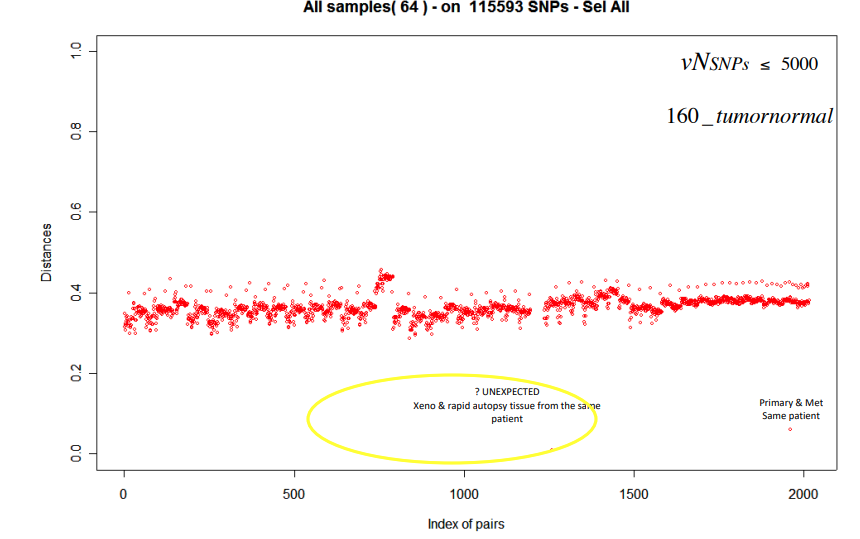
\includegraphics[width=0.7\textwidth]{loci3.PNG}
			\caption{Genetic Distance graph with tumour samples}
			\label{fig:Distance3}
		\end{figure}

		Figure \ref{fig:Distance3} depicts a genetic fingerprinting experiment performed on a collection of $160$ tumour samples, with a SNP array composed of more thant $100000$ SNPs.
		Two samples with very low distance can be observed.
		One of the is from a Rapid Autopsy program and the other from a xenograft model.
		Rapid autopsy programs or	RAP are programs for which patients at the end of their life agree to donate their tumour tissues for research purposes.
		The material must be taken within two hours after death.
		Those sample are usually highly characterized but the patient's identity is lost.
		So the metastasis model used for the xenograft was the one obtained from the RAP.

	\subsection{Distance changes with different numbers of SNPs}

	\begin{figure}[H]
		\centering
		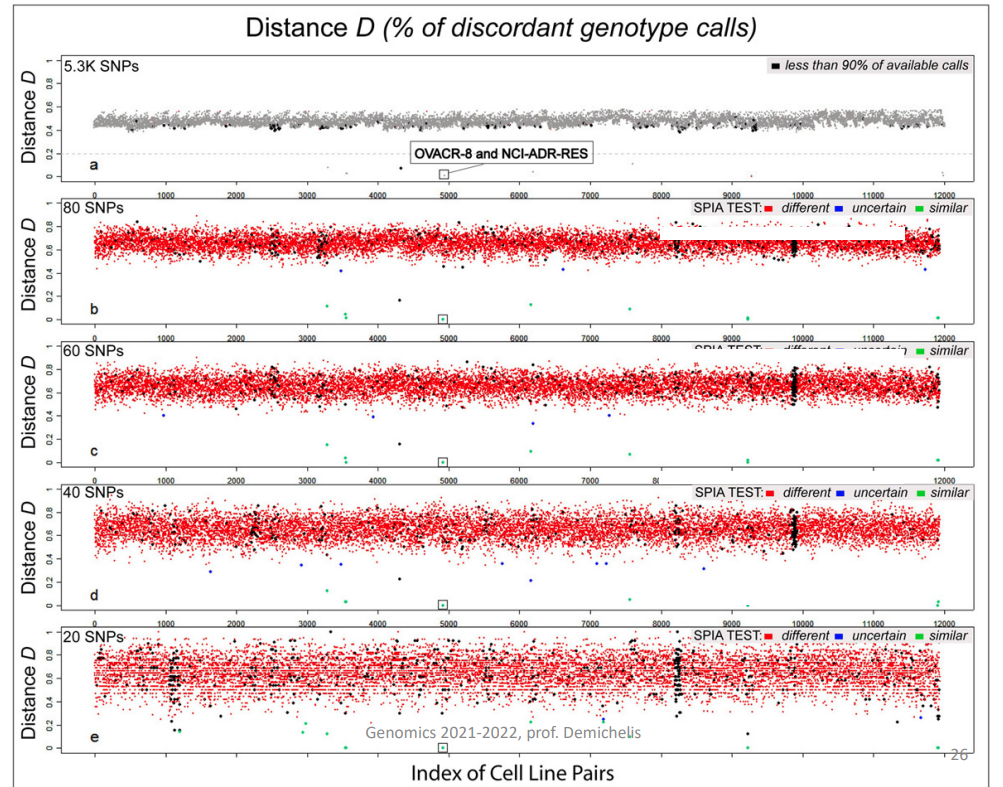
\includegraphics[width=0.7\textwidth]{selected.PNG}
		\caption{Genetic Distance graph at decreasing number of selected SNPs}
		\label{fig:sel_snp}
	\end{figure}

	Figure \ref{fig:sel_snp} depicts an experiment in which the genetic distance among many samples, with an array of $5.3K$ SNPs, was measured using a decreasing number of SNPs from the initial total number of SNPs to decreasing numbers of highly selected SNPs.
	It is noticeable that, in the second plot where $80$ SNPs matching the required characteristics were selected, the average distance and the standard deviation across all pairs is higher than in the previous example, in which all available SNPs were used.
	Decreasing the number of SNPs to 60, then to 40 and 20 leads to have the same average distance between pairs, which settles around 0.66, but higher standard deviation.
	So enough SNPs in order to prevent unexpected issues and to trust the measure are needed.
	Maximizing the likelihood that SNPs have a different genotype, the average distance of unrelated individuals will increase.

\section{Building a SNP-based genetic test}

	\subsection{Pipeline}
	Building an identity test base on SNPs is a multi-step process, consisting in:

	\begin{multicols}{2}
		\begin{enumerate}
			\item Definition of a genetic distance to compare samples.
			\item Definition of SNPs requirements, based on the intention of the assay.
			\item Selection of SNPs:
			\begin{itemize}
				\item This can be done in a data-driven manner, through an iterative procedure of training and test on known sample set;
				\item MAF and Hardy-Weinberg equilibrium from HapMap data.
			\end{itemize}
			\item Implementation of a probabilistic test of classification.
			\item In silico validation on independent datasets.
			\item Validation on cell lines genotyped on independent platform.
		\end{enumerate}
	\end{multicols}

	\subsection{Implementation of a probabilistic test to identify samples}
	When classifying samples there is a need to assess the threshold on the genotype distance to assign samples to a class, the confidence of the classification and the minimum number of loci needed for a robust test.
	A probabilistic test could be used to define the threshold and the confidence.
	The gold standard to do so is to compare observation with expectations.
	Assuming that SNP calls at different loci are independent, this process can be modelled as a binomial distribution: each SNP call is a trial, with $n$ the number of SNPs in the assay, $k$ the number of matches, $p$ the probability of a match and $1-p$ the probability of a mismatch.
	The probability of having $k$ matches out of $n$ SNPs follows a binomial distribution.
	Moreover with $n$, $np$ and $np(1-p)$ large enough, the Gaussian approximation of the binomial distribution can be used.
	Doing so the probability of having $k$ matches out of $n$ SNPs can be modelled as a Gaussian distribution with:

	$$\mu = np\qquad\land\qquad \sigma = np(1-p)$$

	The area of confidence o the assay can be defined as $1m\pm m\cdot \sigma$, where $m$ is the number of standard deviations used to define the threshold.

		\subsubsection{Classification}

		\begin{figure}[H]
			\centering
			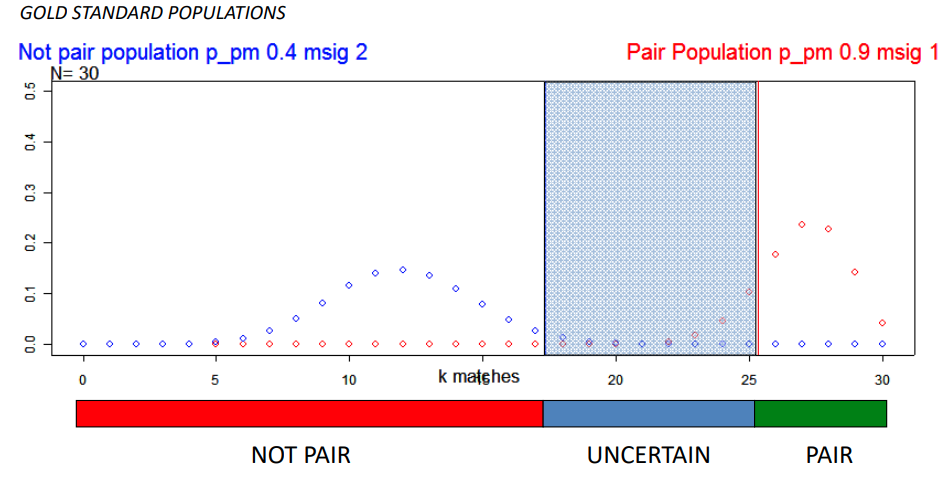
\includegraphics[width=0.7\textwidth]{double_test.PNG}
			\caption{}
			\label{fig:prob_test}
		\end{figure}

		Having modelled the match distribution, the probability mass function for unrelated individual (blue dotted line in figure \ref{fig:prob_test}) can be plotted
		The same can be done with the probability mass function for related individual (red dotted line in figure \ref{fig:prob_test}).
		These functions can be used to set thresholds to define $3$ regions dependent on the number of matche:

		\begin{multicols}{3}
			\begin{itemize}
				\item Not pair: samples in this region are different.
				\item Pair: samples in this regions are similar.
				\item Uncertain: no certain result.
			\end{itemize}
		\end{multicols}

		The grey area changes with $m$ and defines the level of confidence.
		Decreasing the number of SNPs the grey zone will decrease, making the results difficult to interpret.

	\subsection{Some examples of genetic tests}

		\subsubsection{Investigating cell line passages}
		A massive use of these genetic tests is done to assess genetic changes during in-vitro cultivation  and in studies for tumor evolution, lineage plasticity and heterogeneity across metastasis across individuals or in single tumor.
		Cell lines go through multiple passages in which they are used and stored.
		Genetic fingerprinting can be used to assess if among different passages the cells have remained the same, if they were mislabeled or if major genetic drifts happened.

		\begin{figure}[H]
			\centering
			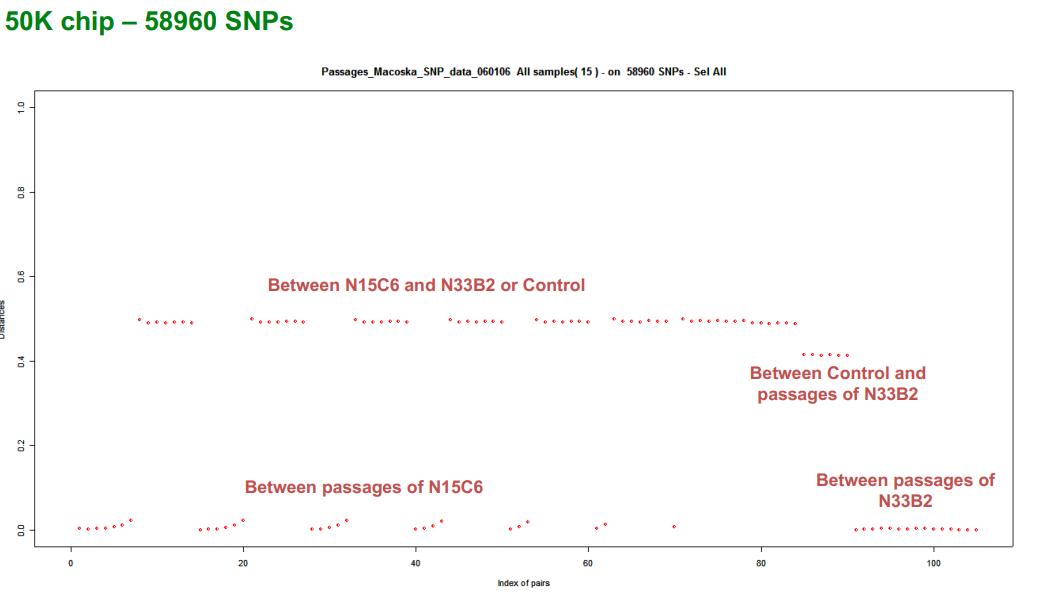
\includegraphics[width=0.4\textwidth]{50k.png}\quad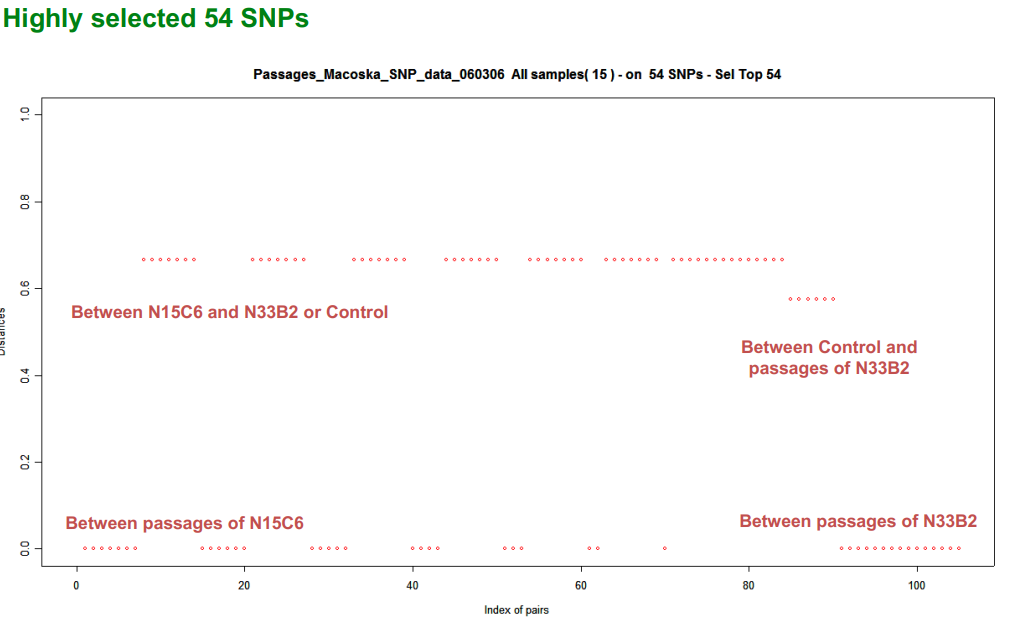
\includegraphics[width=0.4\textwidth]{54_snps.PNG}
			\caption{Genetic distance between cell line passages}
			\label{fig:cell_lines}
		\end{figure}

		In the example \ref{fig:cell_lines}, two types of prostate cell lines which underwent multiple passages were used:

		\begin{multicols}{2}
			\begin{itemize}
				\item $N15C6$ from passages from $48$ to $63$.
				\item $N33B2$ from passages from $21$ to $39$.
			\end{itemize}
		\end{multicols}

		The cell lines were profiled with a SNPs array and a genetic fingerprinting test was performed.
		All passages of each cell lines were compared with all other passages.
		All passages from the same cell line should be classified as similar in the test.
		However the results obtained using the full array of SNPs (50k), showed that some pairs which should be exactly identical are different.
		They can be seen on the bottom-left of \ref{fig:cell_lines}.
		Using only $54$ SNPs this distance is not detectable.
		This increased distance is due to a major difference for certain passages with respect to the initial one on chromosome $11$ of $N15C6$.
		This is due to the insertion in chromosome $11$ of a viral sequence to immortalize the cell line.

		\subsubsection{Investigating individual relatedness}
		The HapMap consortium sequenced hundreds of individuals and trios for different ethnicities and also used trios.
		Trio sequencing is a technique which involves the sequencing of the genome of mother, father and their child.
		Trios provide major information of haplotype blocks and for identifying regions related to inheritance.

		\begin{figure}[H]
			\centering
			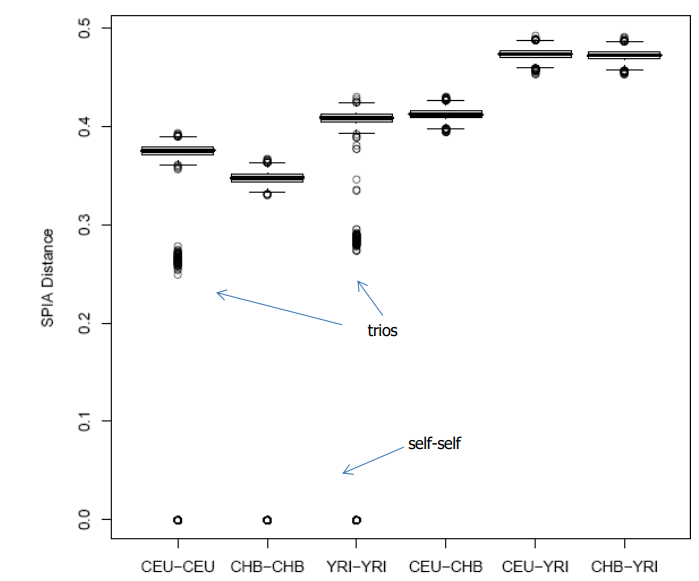
\includegraphics[width = 0.7\textwidth]{relatedness.PNG}
			\caption{Trio genotype distance}
			\label{fig:trios}
		\end{figure}

		Figure \ref{fig:trios} depicts the genetic distance of individuals computed by the SPIA Assay.
		Self-self pairs have a genetic distance of $0$.
		Each ethnicity has an average genetic distance different from the global one and trios have a lower distance from individual from the same ethnicity.
		Different in MAF in population could explain differences in distance among mixed samples.
		This shows how this type of test can be used for paternity tests of for forensic science.

	\subsection{Genetic structure of the human population}
	One relevant aspect of the human genome is that it contains everything needed to learn about the genetic structure of the human population.
	Understanding the genetic structure of human populations is of fundamental interest to medial, forensic and anthropological sciences.
	Knowing the genetic substructure of data is important because:

	\begin{multicols}{2}
		\begin{itemize}
			\item The goal of association studies is to identify DNA variants that affect disease risk or other traits of interest.
				However, association studies can be confounded by differences in ancestry.
			\item Misleading results could arise if individuals selected as disease cases have different ancestry, on average, than healthy controls.
				If in a study all controls are of the same ethnicity and the test is done on an individual of a different ethnicity than the test is biased.
			\item If GWAS study using a specific ethnicity a worldwide marker for susceptibility for a molecule or disease cannot be trusted.
		\end{itemize}
	\end{multicols}

In medicine and in the study of human evolution is important to track the genetic background of individuals that are involved in studies in order to understand if the individuals are form a homogeneous population or from genetically distant ones.
More and more, clinical studies must have declarations of the checks and interpretation of the data of the genetic background of the individuals present in the study.
It is very important to come to results for which we know exactly what is the applicability.
To avoid spurious results, association studies often restrict their focus to a single continental group.
Advances in high-throughput genotyping technology have improved the understanding of global patterns of human genetic variation and suggest the potential to use large sample sets to uncover variation among closely spaced populations.
One important piece of information to consider when developing methods to understand the genetic structure of a population is to think in term of variance, which is also relevant for human diseases.
Many SNPs have different MAFs in different populations and those could be used to infer the individual genetic background in terms of origins.
The easiest mathematical approach to assess how well SNPs can distinguish ethnicity is by using \textbf{Principal Component Analysis (PCA)}.
By running a very simple PCA on a set of SNPs including SNPs with different MAF in different populations different ethnical groups can be distinguished.

		\subsubsection{Genes mirror geography in Europe}
		$500k$ single nucleotide polymorphism array was used to genotype samples.
		Information about the country of origin of grandparents, parents and other relatives was used to determine the geographical location that best represents each individual ancestry.
		They run a combined study where they used a supervised search to find the best SNPs to make inference and then they tested it on another set of individuals.
		By using high confidence data (individuals with high confidence origin data) and by using the genotypes of highly informative SNPs for specific region-related inheritance, they were able to rebuild the map of some of the countries in Europe \ref{fig:PCA_countries}.

		\begin{figure}[H]
			\centering
			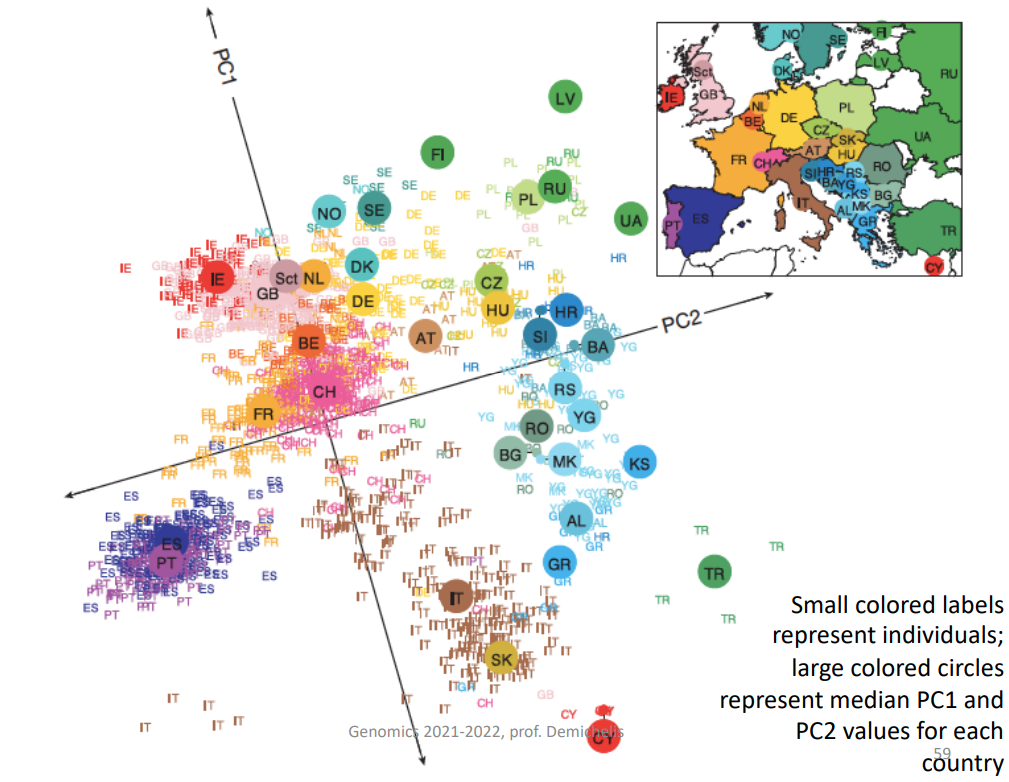
\includegraphics[width=0.7\textwidth]{population.PNG}
			\caption{\label{fig:PCA_countries}}
		\end{figure}

		Properly selecting variants it should be possible to distinguish individuals coming from different countries.
		SNPs were selected following the genetic fingerprinting approach, adding for SNPs with different MAF in different population.
		More dense and distant clusters could be due to the fact that SNPs selected are typical for that area and are able to maximize the difference with respect to it.

		\begin{figure}[H]
			\centering
			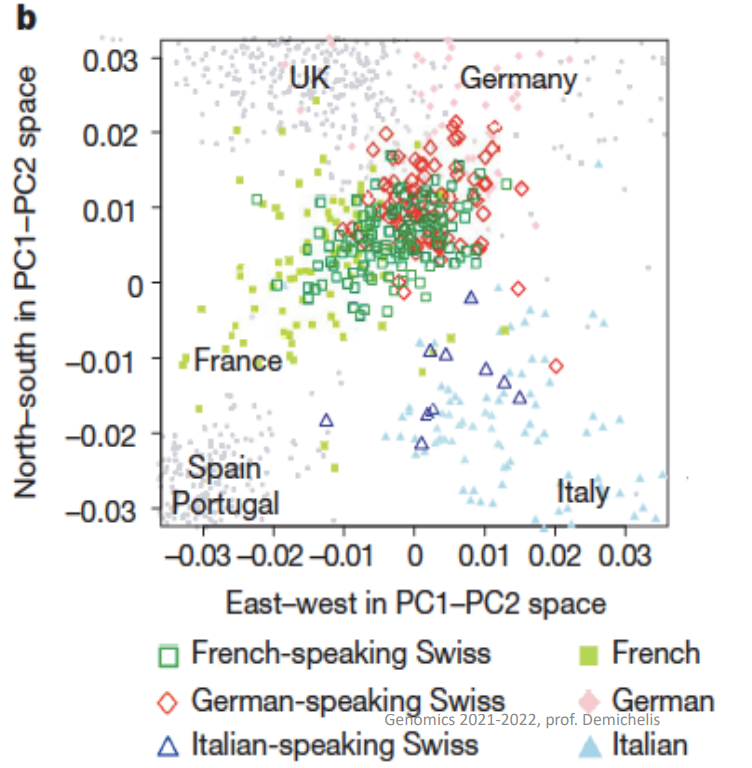
\includegraphics[width=0.5\textwidth]{swiss.PNG}
			\caption{\label{fig: PCA_swiss}}
		\end{figure}

		Focusing on Switzerland, they could even make inference on the linguistic canton \ref{fig: PCA_swiss}.
		It is possibly true that in country where some regions have very different habits might lead to have similar genetic fingerprint.
		Moreover low-frequency alleles tend to be the result of a recent mutation and are expected to geographically cluster around the location at which the mutation first arose.
		Hence, they can be highly informative about the fine-scale population structure.
		Despite low average levels of genetic differentiation among Europeans, close correspondence between genetic and geographic distances was found.
		When mapping the genetic basis of a disease phenotype, spurious associations can arise if genetic structure is not properly accounted for.

    \graphicspath{{chapters/notes/04/images}}
\chapter{IGV (Integrative Genomics Viewer)} \label{chap: IGV}

\section{IGV characteristics}

    \subsection{Introduction}
    The human genome nowadays is being explored extensively thanks to:

    \begin{multicols}{2}
        \begin{itemize}
            \item Exons and whole-genome sequencing.
            \item Epigenetic surveys.
            \item Expression profiling of coding and noncoding RNAs.
            \item SNPs and copy number profiling.
            \item Functional assays.
        \end{itemize}
    \end{multicols}

    IGV allow to visually explore the data generated from this kind of study, which is mostly used for the development of precision medicine, an approach for disease treatment and prevention that takes into account individual variability in:

    \begin{multicols}{3}
        \begin{itemize}
            \item Genes.
            \item Living environment.
            \item Lifestyle.
        \end{itemize}
    \end{multicols}

    The objective of precision medicine is to define which drug, at what time and at what dose to administer to an ill individual to have optimal response.
    The IGV software is a high-performance lightweight visualization tool for interactive exploration of large, integrated genomic datasets.
    It supports a wide variety of data types, including next-generation sequence data, and genomic annotations.
    Data sets can be loaded from local or remote sources, including cloud-based resources.
    In IGV, each vertical bar corresponds to a read.
    A coloured sign in a read indicates the presence of a polymorphism.
    The browser also gives info about the quality of the read and the bases from the loaded BAM file.
    Other information regarding IGV are present in the \href{https://authors.library.caltech.edu/72234/2/nbt.1754-S1.pdf}{Supplementaty information - Integrative Genomics Viewer} pdf file.

    \subsection{Main uses of IGV}
    Some utilization of IGV are:

    \begin{multicols}{2}
        \begin{itemize}
            \item NGS alignment.
            \item Epigenomics studies.
            \item Copy number evaluations.
            \item RNA-sequencing.
            \item Identification of variants and genotypes.
        \end{itemize}
    \end{multicols}

    Some of the main utilization are represented in figure \ref{fig:IGVusages}.

    \begin{figure}[H]
        \centering
        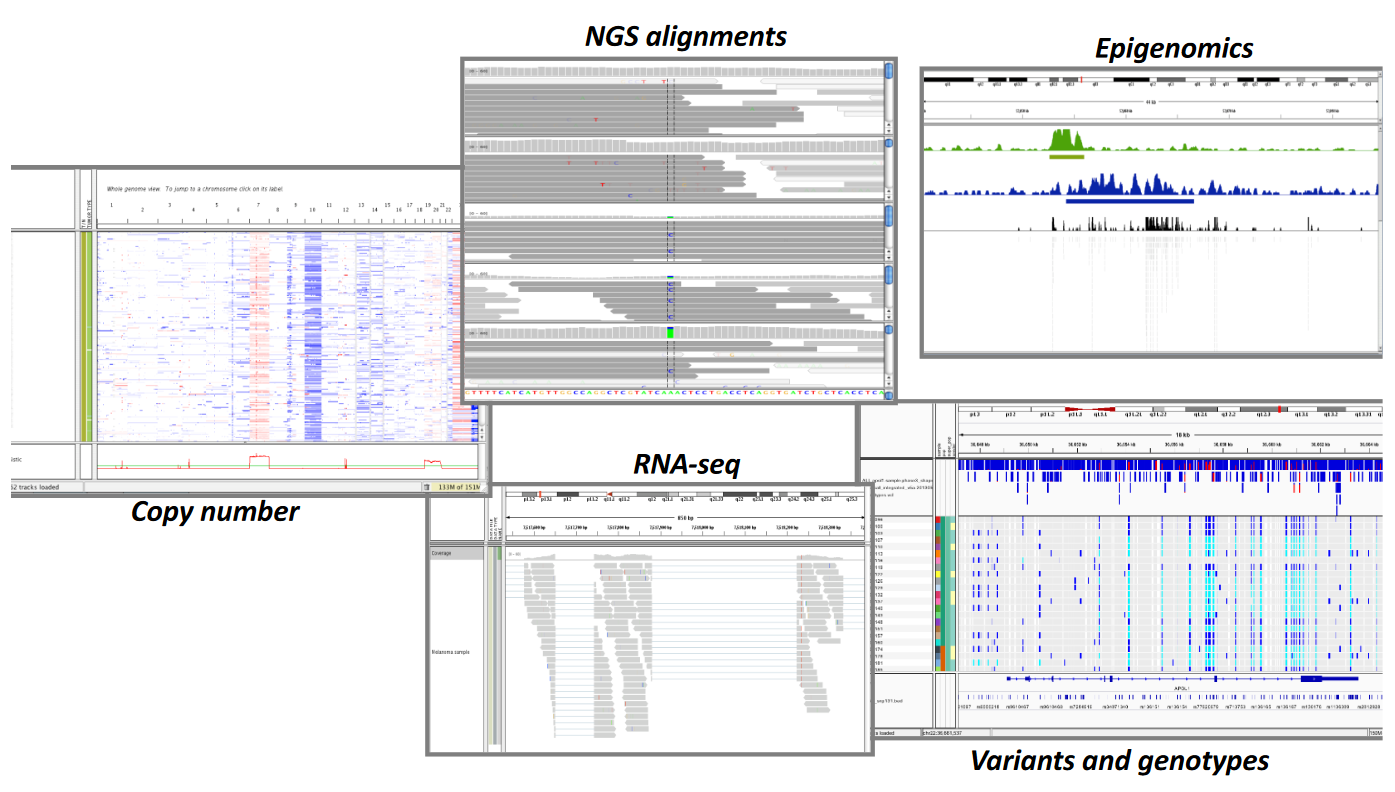
\includegraphics[width=0.8\textwidth]{usagesIGV.PNG}
        \caption{Main type of data exploration done with IGV.}
        \label{fig:IGVusages}
    \end{figure}

        \subsubsection{RNA sequence analysis}
        IGV can be used to explore RNA sequence analysis.
        For example figure \ref{fig:RNAseq} represents reads that span exon junctions, with their heights depending on the number of reads that connect them.

        \begin{figure}[H]
            \centering
            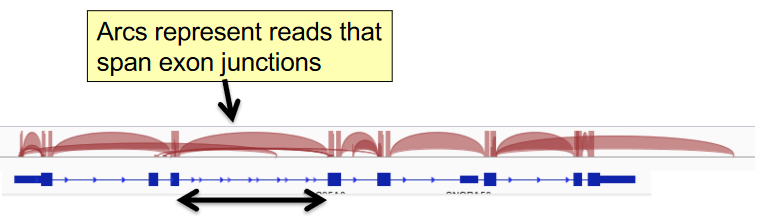
\includegraphics[width=0.7\textwidth]{RNAseqAlign.PNG}
            \caption{View of RNA sequence data for a gene.}
            \label{fig:RNAseq}
        \end{figure}

        Another thing that can be done are Sashami plots.
        In these plots the number of reads connecting exosomes are represented on curved lines.
        The peaks represents coverage within exons.
        An example of a Sashami plot is depicted in figure \ref{fig:sashami}.

        \begin{figure}[H]
            \centering
            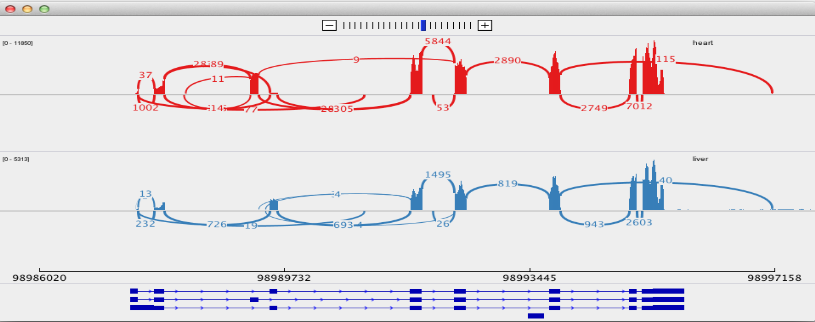
\includegraphics[width=0.8\textwidth]{sashamiplot.PNG}
            \caption{Sashami plots}
            \label{fig:sashami}
        \end{figure}

        \subsubsection{Variant discovery}
        IGV allows to study variants from different samples, like it can be seen in figure \ref{fig:variants}

        \begin{figure}[H]
            \centering
            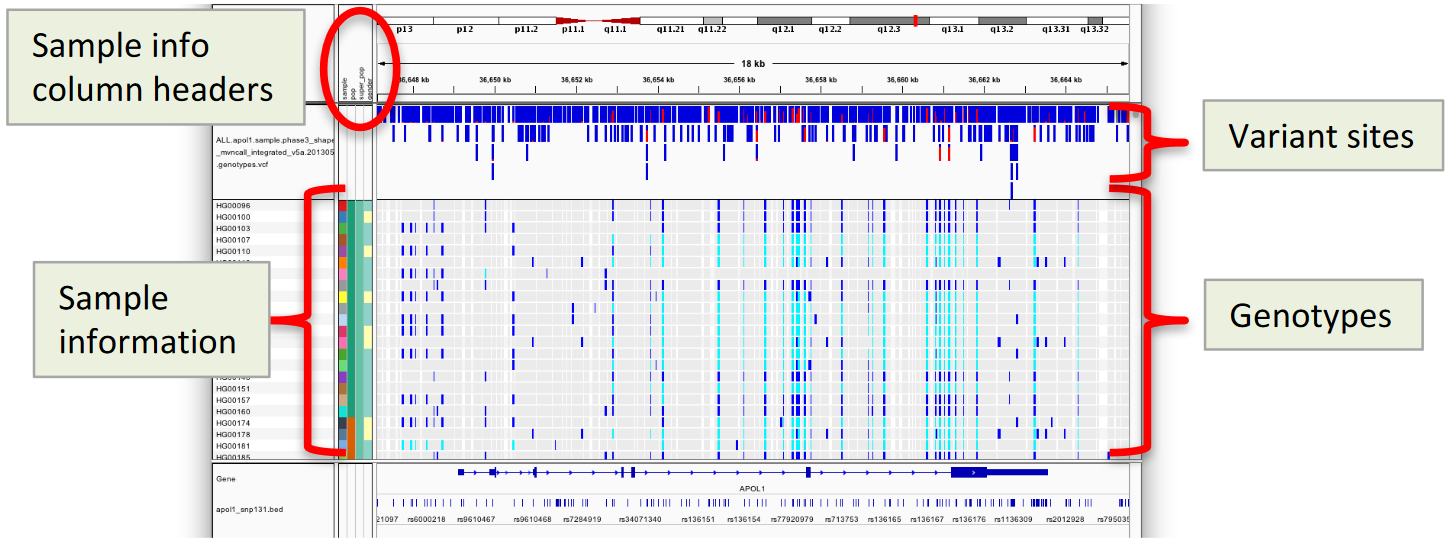
\includegraphics[width=0.9\textwidth]{variantsView.PNG}
            \label{fig:variants}
        \end{figure}

    \subsection{Operations}
    IGV allows for the simultaneous visualization of an arbitrary number of BAM files.
    The user can move, zoom in and out quickly over different genomic scales, panel \emph{a} of figure \ref{fig:IGV_navigation}), and also to jump in precise positions of the sequence.
    It is possible to search for genomic coordinates or gene names.
    For each resolution scale called zoom levels, the aggregated data is divided into tiles, panel \emph{b} of figure \ref{fig:IGV_navigation}) that correspond to a region viewable on a typical user display.
    Each tile is subdivided into bins, with the width of a bin chosen to correspond to the width represented by a pixel at that resolution scale.
    It is also possible to sort the samples in different ways and to group them considering different characteristics.


    \begin{figure}[H]
        \begin{tabular}{cc}
          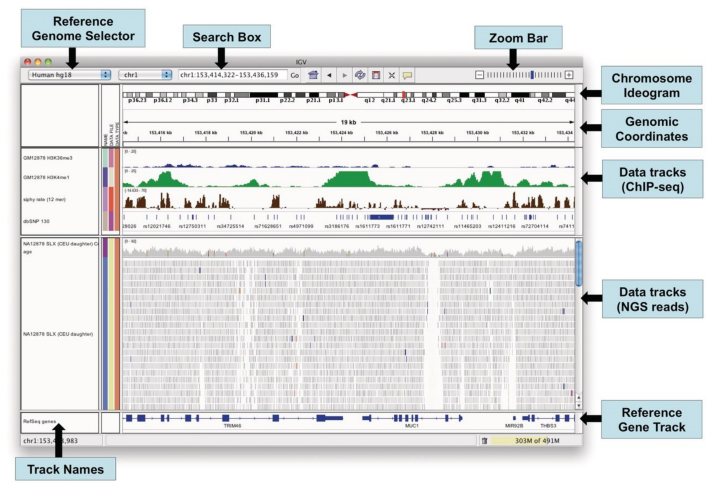
\includegraphics[width=0.5\textwidth]{IGVview.PNG} &   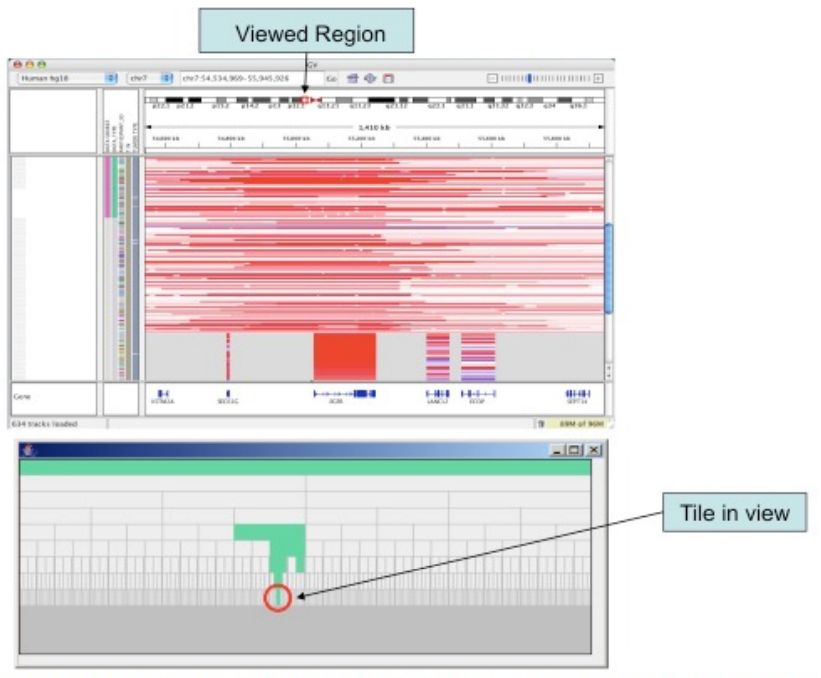
\includegraphics[width=0.5\textwidth]{TileView.PNG} \\
        (a) IGV interface main features & (b) Tiles view in IGV \\[6pt]
        \end{tabular}
        \caption{}
        \label{fig:IGV_navigation}
    \end{figure}

    Navigation through a data set is similar to that of \textit{Google Maps}, allowing the user to zoom and pan seamlessly across the genome at any level of detail from whole genome to base pair.
    Annotations for specific genomes could be found consulting the UCSC Table Browser \href{http://genome.ucsc.edu/cgi-bin/hgTables}{(UCSC table)}.\\

    \subsection{Tiles}
    The corresponding data tiles for each zoom level are stored in the binary Tiled Data Format, or TDF, which has been optimized for fast tile retrieval.
    A tiled data file (.tdf) is a binary file that contains data that has been preprocessed for faster display in IGV.
    TDF files are generated by using the \textit{igvtools} package (\textit{toTDF} command).
    Tile sizes for each zoom level are constant and small.
    A single tile at the lowest resolution (spanning the entire genome) has the same memory footprint as a tile at the very high zoom levels (might span only a few kilobases).
    Tiles no longer in view are discarded as needed to free memory.

        \subsubsection{Pixel resolution error}
        Pixel resolution errors occur when data density exceeds the constraint given by the number of pixels available for display.
        This can be solved through data aggregation.
        As the user zooms below the $\sim 50 kb$ range, individual aligned reads become visible, like in figure \ref{fig:ViewReads}.
        It is possible then to zoom further, and see the bases at each position.

        \subsubsection{Data displayed at different resolutions}

        \begin{figure}[H]
            \centering
            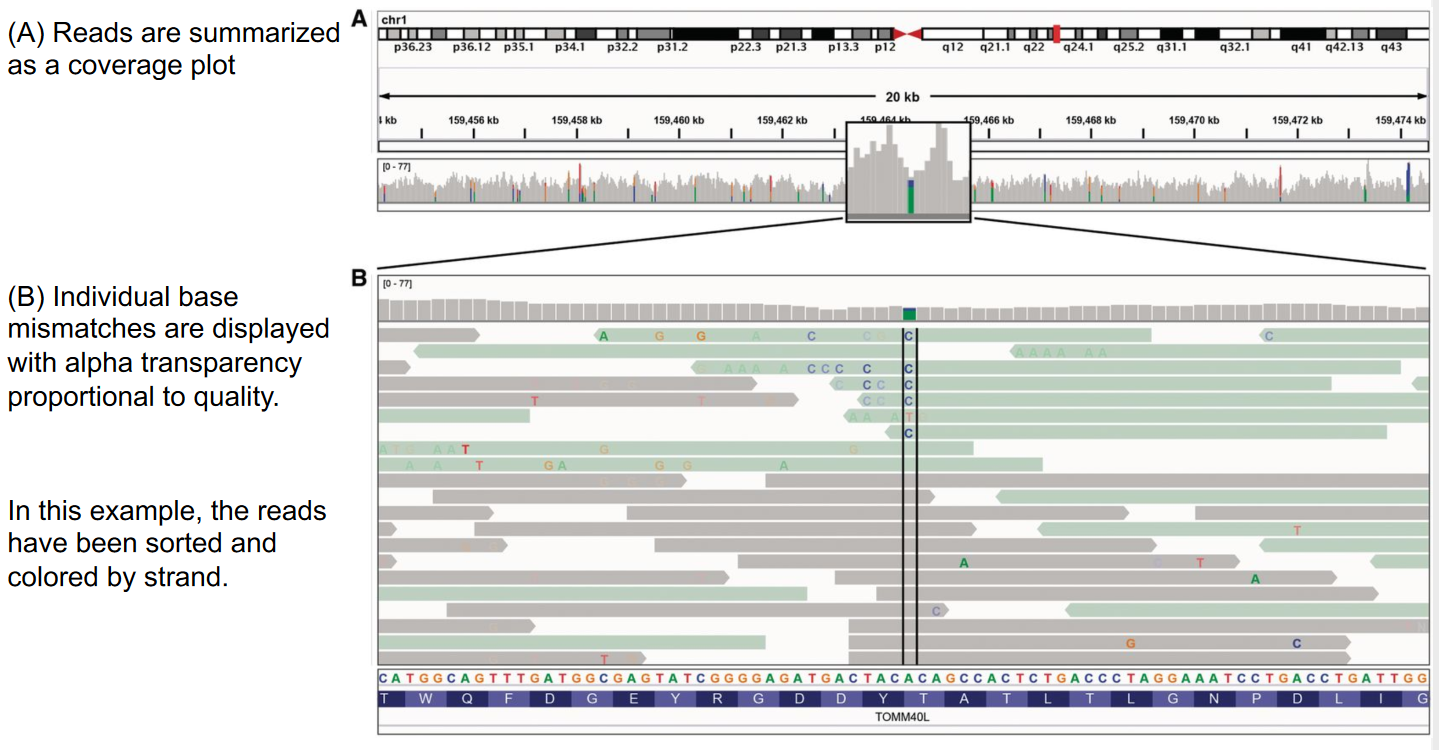
\includegraphics[width=0.7\textwidth]{IGVReadsView.PNG}
            \caption{Different resolution of IGV}
            \label{fig:ViewReads}
        \end{figure}

        In panel a of figure \ref{fig:ViewReads} reads are summarized as a coverage plot.
        In panel b individual base mismatches are displayed with alpha transparency proportional to quality.
        In this example, the reads have been sorted and coloured by strand and span a $20 kb$ genomic region for $1$ individual.
        The coverage is between $0$ and $77$ at certain positions there is more than one base supported by the reads.
        This is visualised by the green and blue column: some reads support $C$ instead of $A$.
        The coloured area is proportional to the allelic fraction for each base.

    \subsection{IGVTools}
    Igvtools comprises a set of utilities to prepare large files for efficient display.
    Some commands are reported in figure \ref{fig:commands}.
    In particular the count function takes as input a BAM file to generate coverage data.
    The obtained file could be then loaded with the "Load pre-computed coverage data" command for faster loading times.

    \begin{figure}[H]
        \centering
        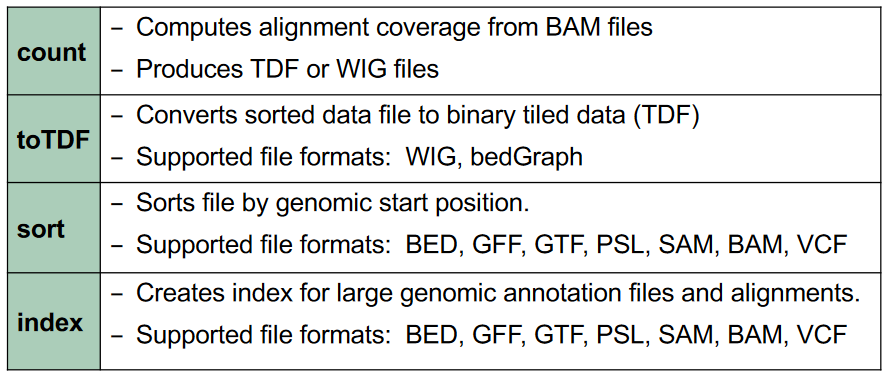
\includegraphics[width=0.6\textwidth]{igvtools.PNG}
        \caption{igvtools possible operations.}
        \label{fig:commands}
    \end{figure}

    \subsection{Session files}
    Sessions allow users to share their data and views with other users simply and accurately.
    Session files describe the session state in XML.

\section{Interpreting pair orientations}
IGV allows to discover  genetic aberrations through the interpretation of pair orientation.
A paired end protocol can uncover:

\begin{multicols}{3}
    \begin{itemize}
        \item Inversions.
        \item Duplications.
        \item Translocations.
    \end{itemize}
\end{multicols}

To detect these kind of events reads that span the breakpoint are needed.
This type of reads can be obtained through long reads or paired-end sequencing.

    \subsection{Element to consider when interpreting pair orientations}
    Different parameters are to be considered when interpreting pair orientations:

    \begin{multicols}{2}
        \begin{itemize}
            \item Pair ends relative orientation.
            \item Insert size length.
            \item Coverage within the aberrant region.
            \item Coverage outside of the aberrant region (flanking genomic segments).
            \item Coverage at the breakpoints.
        \end{itemize}
    \end{multicols}

    In particular when considering pair ends relative orientation some considerations can be done:

    \begin{multicols}{2}
        \begin{itemize}
            \item \textbf{LR} ($\rightarrow\cdots\leftarrow$): is an Illumina convention, and implies that the reads are left and right of the unsequenced part of the sequenced DNA fragment when aligned back to the reference genome.
            \item \textbf{LL}, \textbf{RR} ($\leftarrow\cdots\leftarrow\land\rightarrow\cdots\rightarrow$): implies an inversion in sequenced DNA with respect to the reference.
            \item \textbf{RL} ($\leftarrow\cdots\rightarrow$): implies a duplication or translocation with respect to the reference.
        \end{itemize}
    \end{multicols}

    \subsection{Inversion}
    Figure \ref{fig:inversion} depicts an inversion.
    A local drop in coverage and reads direction $LL$ or $RR$ can be observed.
    Moreover a drop on the breakpoint can be observed.

    \begin{figure}[H]
        \begin{tabular}{cc}
            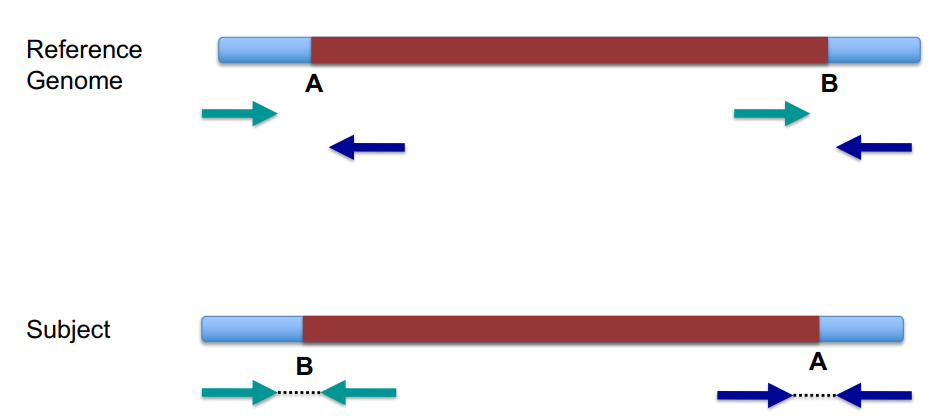
\includegraphics[width=0.5\textwidth]{inversion.png} &   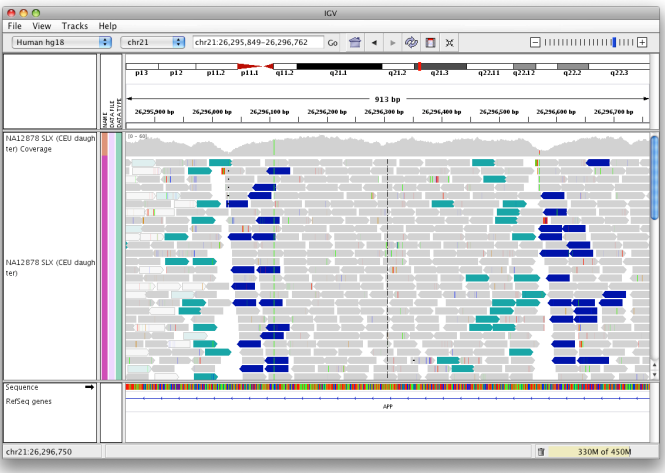
\includegraphics[width=0.5\textwidth]{inversion_igv.png} \\
            (a) Schematic & (b) IGV view \\[6pt]
        \end{tabular}
        \caption{Inversion discovering exploiting PE reads.}
        \label{fig:inversion}
    \end{figure}

    \subsection{Tandem duplication}
    Figure \ref{fig:tandem} depicts a tandem duplication.
    All the reads that do not cover the junction point align perfectly to the reference.
    Moreover it can be observed a $50\%$ increase of coverage proportional to the extra copy.
    Junctions $A$ and $B$ are not modified.
    A read mapping $BA$ would be partially aligned at $B$ on the reference.
    There is no drop in coverage.


    \begin{figure}[H]
        \begin{tabular}{cc}
            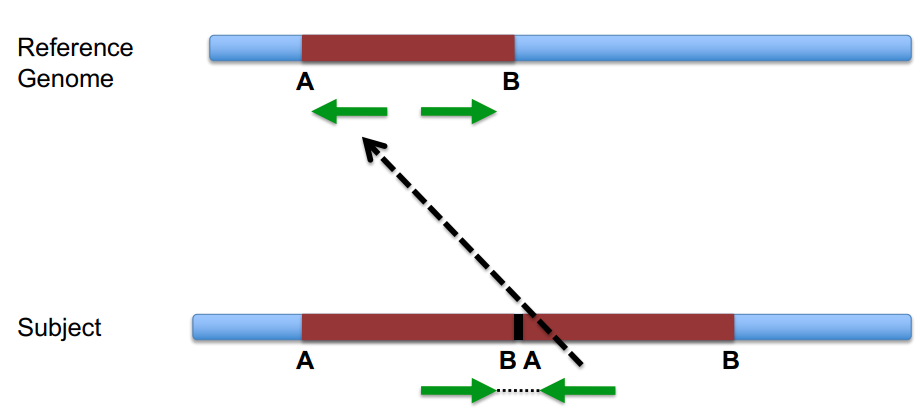
\includegraphics[width=0.5\textwidth]{tandem.png} &   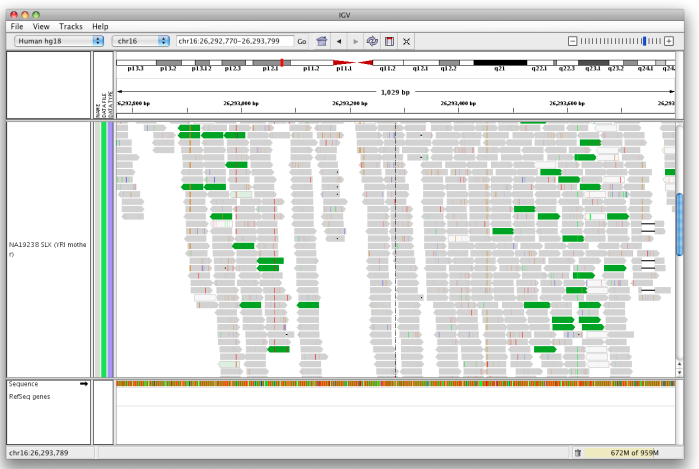
\includegraphics[width=0.5\textwidth]{tandem_igv.png} \\
            (a) Schematic & (b) IGV view \\[6pt]
        \end{tabular}
        \caption{Tandem duplication discovering exploiting PE reads.}
        \label{fig:tandem}
    \end{figure}

    \subsection{Inverted duplication}
    Figure \ref{fig:inverted} depicts an inverted duplication.
    Coverage increase in the duplicated site in the reference gene is expected.
    Both $A$ and $B$ on the first segment are $LR$, while the second will have reads oriented $LL$ or $RR$.
    The insert size will be significantly longer.
    An overlapping of left and right reads can be found on the reference.

    \begin{figure}[H]
        \begin{tabular}{cc}
            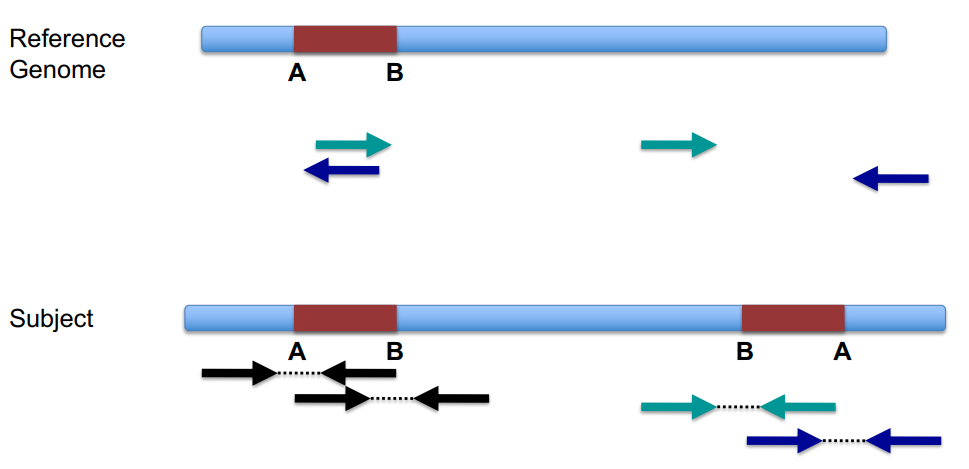
\includegraphics[width=0.5\textwidth]{inverted.png} &   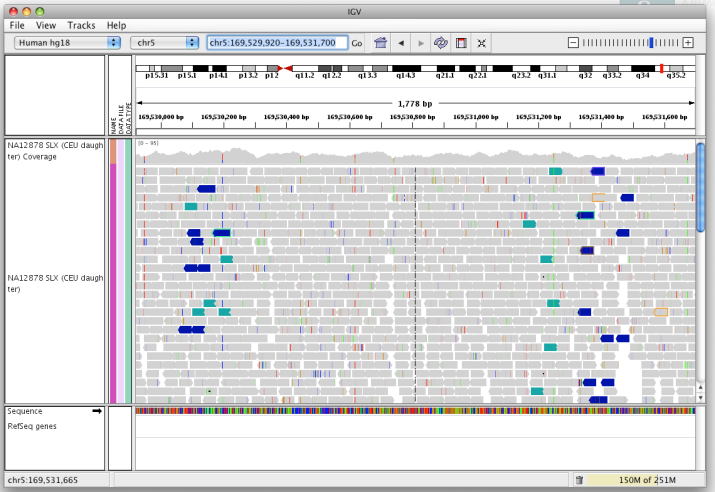
\includegraphics[width=0.5\textwidth]{inverted_igv.png} \\
            (a) Schematic & (b) IGV view \\[6pt]
        \end{tabular}
        \caption{Inverted duplication discovering exploiting PE reads.}
        \label{fig:inverted}
    \end{figure}

    \subsection{Deletion}
    Deletion can be discovered by observing drop in coverage or the observed distance between reads, which gives a clean indication of the size of the deletion.
    For small deletions like indels the sequence within the reads has to be observed.

\section{Uncovering genetic aberrations - some examples}

    \subsection{First example}
    Figure \ref{fig:task_a} depicts the genomic region chr1:11,050,009-11,055,137.
    The event visualized could be a tandem duplication on one of the two alleles and a deletion on the other allele.
    This is due to the fact that despite of the duplication the coverage on remains constant on the region.

    \begin{figure}[H]
        \centering
        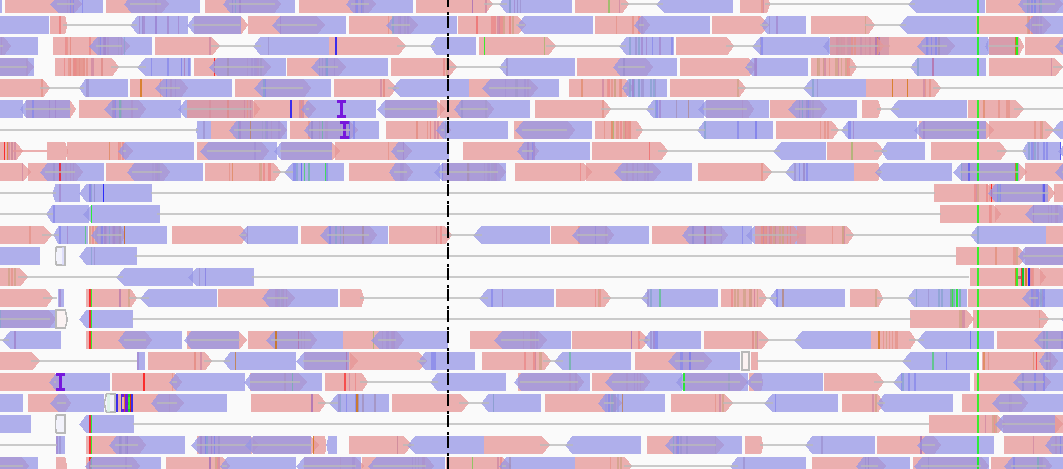
\includegraphics[width=0.8\textwidth]{pos1.PNG}
        \caption{A tandem duplication followed by a deletion}
        \label{fig:task_a}
    \end{figure}

    \subsection{Second example}
    Figure \ref{fig:task_b} depicts the genomic region chr5:9,410,315-9,413,699.
    It is clear due to the absence of coverage how both allele of that region were deleted.

    \begin{figure}[H]
        \centering
        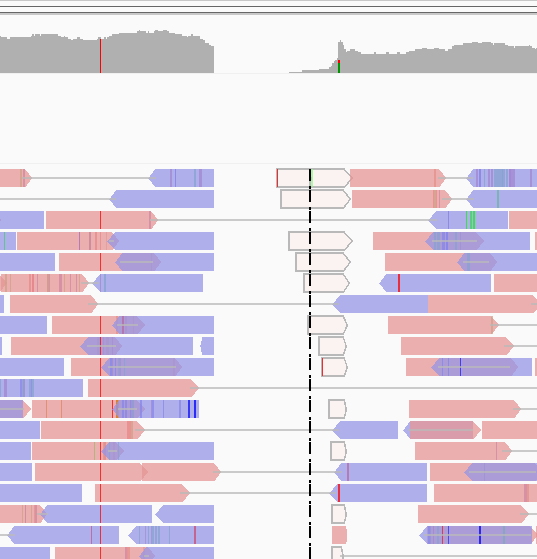
\includegraphics[width=0.6\textwidth]{pos2.PNG}
        \caption{An homozygous deletion}
         \label{fig:task_b}
    \end{figure}

    \subsection{Third example}
    Figure \ref{fig:cov3} and \ref{fig:ex_3} depicts an inverted duplication followed by a deletion.
    This prediction is justified because of the presence of overlapping $LR$ reads and $LL$ and $RR$ reads with a correspondent increase of coverage, followed in the following region by a considerable drop in coverage, indicating an heterozygous deletion.

    \begin{figure}[H]
       \centering
       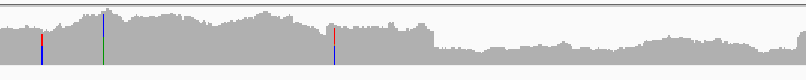
\includegraphics[width=1\textwidth]{cov3.PNG}
       \caption{Coverage for an inverted duplication followed by a deletion}
       \label{fig:cov3}
    \end{figure}


    \begin{figure}[H]
        \begin{tabular}{cc}
        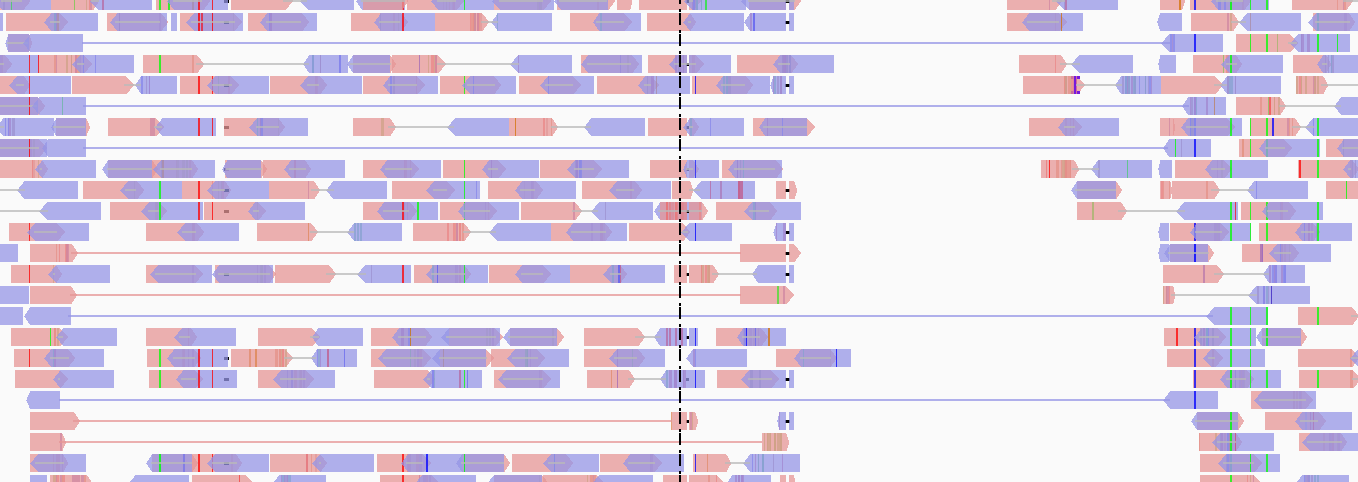
\includegraphics[width=0.5\textwidth]{pos3.PNG} &   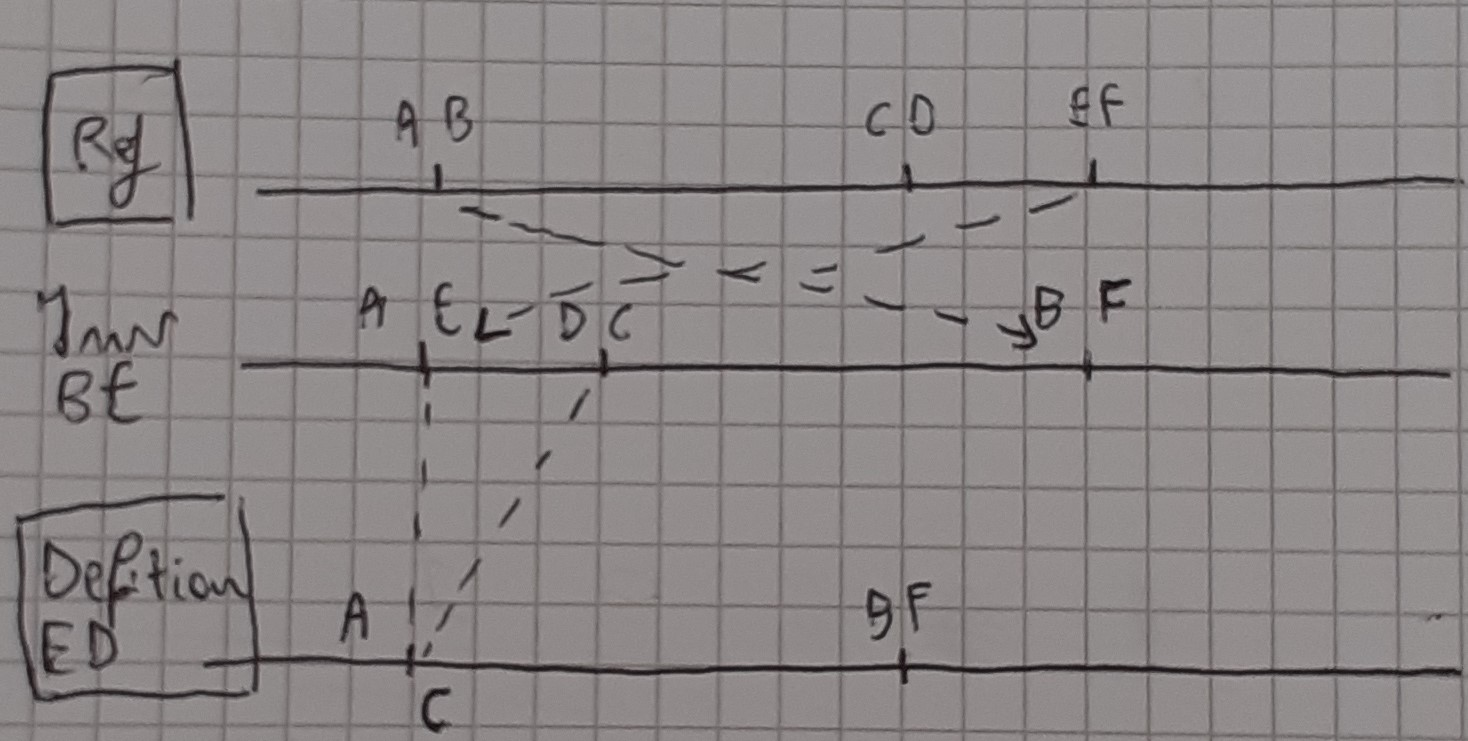
\includegraphics[width=0.5\textwidth]{pos3passages.jpg} \\
        (a) IGV view & (b) written passages \\[6pt]
        \end{tabular}
        \caption{Coverage for an inverted duplication followed by a deletion}
        \label{fig:ex_3}
    \end{figure}

    \graphicspath{{chapters/notes/05/images}}
\chapter{Tumor Evolution Studies via NGS data}

\section{Tumour evolution}

	\subsection{Introduction}
	To be fully able to treat cancer it is important to understand what are the somatic events that occur during tumor genesis and evolution and when they arise.
	Cancer cells accumulate mutations due to both cell division and toxic agents like radiations or UV light.
	These mutations are maintained by the cell and lead to clonal expansion.
	Cancer could then originate or evolve through an arbitrary number of driver mutations that could, for example, activate an oncogene or disrupt some molecular pathways.

		\subsubsection{Typical traits of cancer}
		Typical traits of cancer are:

		\begin{multicols}{2}
			\begin{itemize}
				\item Cancer is a dynamic disease: tracking its evolution if fundamental.
				\item During the course of disease, cancers generally become more heterogeneous, which is often related to treatment resistance.
				\item The bulk tumour includes a diverse collection of cells harbouring distinct molecular signatures with differential levels of sensitivity to treatment.
				\item This heterogeneity might result in a non-uniform distribution of genetically distinct tumour-cell sub-populations across and within disease sites (spatial heterogeneity) or temporal variations in the molecular make-up of cancer cells (temporal heterogeneity).
			\end{itemize}
		\end{multicols}

		\subsubsection{Tumour boards}
		Tumour boards are teams of specialists that follow a cancer patient through treatment.
		They collect data and suggest course of actions during the illnesses and can teach new doctors how to manage difficult cases.

	\subsection{Heterogeneity}
	Every site of the genome with somatic mutations is going to be differentially represented in tumour samples.
	Heterogeneity drives cancer resistance and is a great obstacle in treatment.
	Therefore, an accurate assessment of tumour heterogeneity is essential for the development of effective therapies.
	Emerging techniques to study with considerable potential to dissect the complex clonal architecture of cancers heterogeneity are:

	\begin{multicols}{2}
		\begin{itemize}
			\item Multi-region sequencing.
			\item Single cell sequencing.
			\item Analysis of autopsy samples.
			\item Longitudinal analysis of liquid biopsy samples.
		\end{itemize}
	\end{multicols}

	However, techniques to study tumour heterogeneity are hindered by intra-patient heterogeneity, which can be spatial or temporal.
	Figures \ref{fig:hetero} describes tumour heterogeneity.

	\begin{figure}[H]
		\centering
		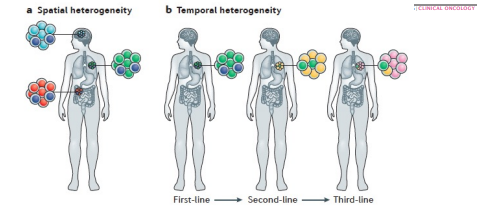
\includegraphics[width=0.7\textwidth]{heterogeneity.png}
		\caption{a) Spatial heterogeneity denotes an uneven distribution of cancer subclones across different regions of the primary tumour and/or metastatic sites. b) Temporal heterogeneity refers to variations in the molecular make-up of a single lesion over time, either as a result of natural progression of the tumour or as a result of exposure to selective pressures created by clinical interventions. Colours denote the presence of subclones with different genetic features.}
		\label{fig:hetero}
	\end{figure}

		\subsubsection{Temporal heterogeneity}
		Temporal heterogeneity refers to the change in time of a single tumour mass.
		This can happen naturally or under particular selective pressures.

		\subsubsection{Spatial heterogeneity}
		Spatial heterogeneity describes different independent tumour masses that can be found in patients which share certain cells while having a unique genetic make-up.

	\subsection{Type of evolutions}
	It could be possible that some cells positively respond to treatment and others not, creating a heterogeneous population in the mass.
	The features of this set of cells changes over time.
	This evolution happens either because the new population replaces the older, or there's a branching and the tumour mass becomes heterogeneous.
	Moreover a metastatic mass could have a monoclonal (from one mass) or polyclonal (from different masses) origin.

	\begin{figure}[H]
		\centering
		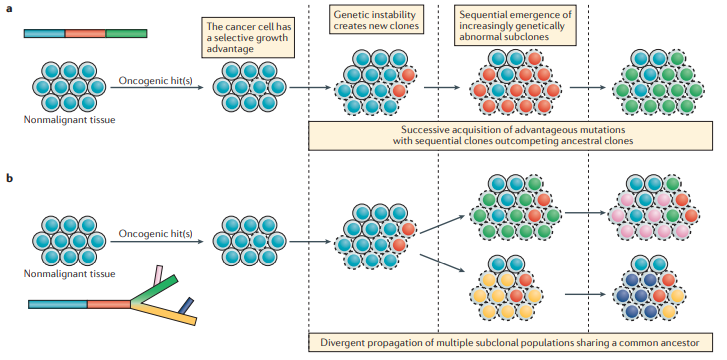
\includegraphics[width=0.7\textwidth]{branching.png}
		\caption{ a) everything branches out from the monoclonal origin, but b) polyclonal origin, independent metastatic processes. Cells from independent lesions meet and form a highly diverse metastatic tumour.}
		\label{fig:branching}
	\end{figure}

		\subsubsection{Linear evolution}
		Sequential genetic alterations confer a fitness advantage such that successive generations are able to out compete the preceding clones, which lack this fitness advantage.
		Surviving dominant clones harbour the ancestral mutation.

		\subsubsection{Branched evolution}
		Multiple genetically distinct populations can emerge from a common ancestral clone, with certain subclonal populations diverging from the common ancestor before others.


	\subsection{Treatment resistance}

	\begin{figure}[H]
		\centering
		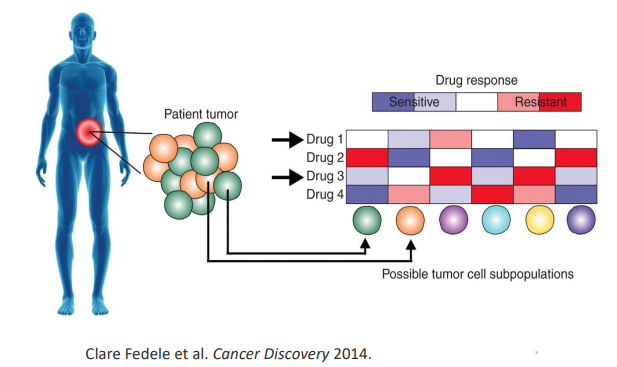
\includegraphics[width=0.6\textwidth]{treatment.png}
		\caption{Certain cells of the tumour mass respond to treatment and some don't. Red cells are resistant to the drug, while blue cells are sensitive to it.}
		\label{fig:treatment_resistance}
	\end{figure}

	Tumour resistance to treatment can be encoded in the original cells or can be driven by the treatment.
	Figure \ref{fig:response} depicts the processes that drive resistance that originates from treatment.
	This can be due to the selection of clones that provide resistance or the transformation of clones under treatment pressure.

	\begin{figure}[H]
		\centering
		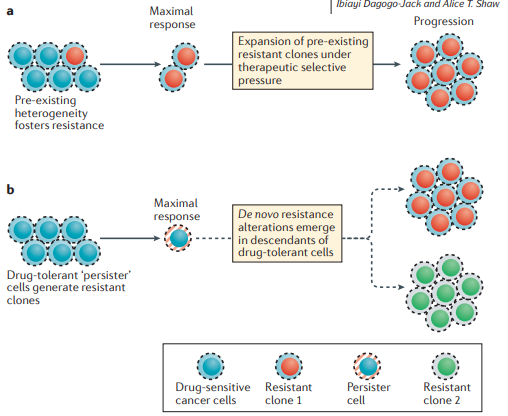
\includegraphics[width=0.7\textwidth]{response.png}
		\caption{ Tumor cells evolution driven by treatment.}
		\label{fig:response}
	\end{figure}

		\subsubsection{Primary resistance}
		Pre-existing heterogeneity fosters resistance.
		Only susceptible cells die and resistant cells continue dividing, allowing the tumour to regrow.
		An high tumour mass will be visible.

		\subsubsection{Acquired resistance}
		Drug-tolerant, persistent cells generate resistant clones.
		At the time of diagnosis there are no markers of the resistance alteration because it is developed afterwards.
		The resistant cells will form over time new tumours not responding to the drug.

\section{Using NGS data to uncover tumour evolution}

	\subsection{Introduction}
	A tumour is a collection of multiple independent lesions.
	Sequencing can be used to obtain a representation of tumour burden and of the features of all of the different areas.
	In order to study tumor evolution common and private lesions across multiple samples from the same individual can be used to reconstruct the evolutionary path.
	Data from multiple individuals can be used, selecting the most clonal lesion, to build a common clonal evolution map.
	From this type of data it has been found, for example that in prostate cancer if CHD1 is mutated, then a subsequent PTNEN mutation is found.
	The interest is on finding which lesions occurred first and which is the model that fits better the data.
	In particular when dealing with tumour data there is a need to take into account:

	\begin{multicols}{2}
		\begin{itemize}
		\item Intra tumor heterogeneity.
		\item Inter tumor/intra patient heterogeneity.
		\item Inter-patient heterogeneity.
		\item Clinical/treatment relevance.
		\item Time dependency.
		\item Admixture DNA (tumor purity).
		\end{itemize}
	\end{multicols}

	This characteristics, if properly investigated, can provide insightful hints during the analysis.

	\subsection{Admixture}
	A sample coming from a patient's tissue contains multiple cell types.
	So a sample will never be composed only of cancer cells.
	DNA admixture refers to the percentage of cells that are not tumoral.
	Purity, instead, is the percentage of cancer cells in a sample.
	It is computed as:

	$$Pur = 1-Adm$$

	A particular lesion is clonal if all tumour cells harbour it.
	If only a portion of cells harbour it it is subclonal.
	Purity and admixture can be used to distinguish between clonal and subclonal lesions.

	\subsection{Informative SNPs}
	SNPs can be exploited to characterize tumour evolution.
	Informative SNPs are heterozygous SNPs: the allelic fraction can be counted and the proportion of reads supporting the alternative base can be assessed.
	The allelic fraction will change for somatic events that involve the genomic locus of a particular SNP, allowing to detect them.
	This is represented in \ref{fig:af_properties}.
	For example in a deletion the allelic fraction of a heterozygous SNP will change from $0.5$ to either $0$ or $1$.
	In particular when selecting informative SNPs to design an assay is important to consider their MAF together with data from databases like dbSNP to select the one that are most probable to are in an heterozygous genotype.

	\begin{figure}[H]
		\centering
		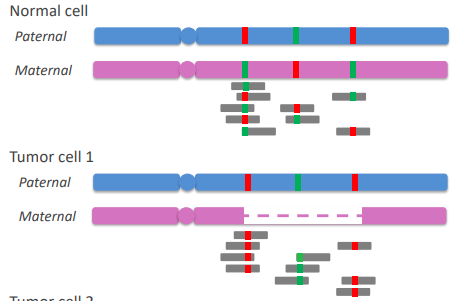
\includegraphics[width=0.5\textwidth]{af_properties.png}
		\caption{Thanks to the presence of informative SNPs is easy to detected the loss of an allele in the tumour cell.}
		\label{fig:af_properties}
	\end{figure}

	\subsection{Beta value}
	When dealing with non pure samples the $\beta$ value needs to be introduced to uncover events concerning informative SNPs.
	This is because the allelic fraction signal will change based on the purity: in fact when only some cells in the sample are from a tumour the allelic fraction distribution will have two peaks.
	$\beta$ is the percentage of neutral reads, or the number of reads that can be coupled, one with the reference base and one with the alternative, over the total number of reads at that SNP.
	In particular:

	\begin{multicols}{2}
		\begin{itemize}
			\item $\beta = 1$ both alleles equally represented.
			\item $\beta = 0$ only one allele represented.
		\end{itemize}
	\end{multicols}

	The more $\beta$ is far from $1$, the more the sample is admixed or the more the lesion is clonal.
	Moreover $Nref$, the percentage of the reference base in the non-deleted allele can be introduced.
	Figure \ref{fig:b_af_purity} links together the concepts of $\beta$, sample purity and allelic fraction.

	\begin{figure}[H]
		\centering
		\includegraphics[width=0.8\textwidth]{a.png}
		\includegraphics[width=0.8\textwidth]{b.png}
		\caption{A)Example of the allelic fraction (AF) and beta ($\beta$) computed in five genomic positions ($p_1$ to $p_m$).
			Positions $p_1$ to $p_n$ are within a hemizygous deleted genomic segment A, while genomic positions $p_{n+1}$ to $p_m$ lie within a wild type genomic segment B.\\
			B-D) Examples of a normal cell and two different tumor cells.
			Tumor cells 1 and 2 differ for the status of genomic segment B.
			Histograms below cell cartoons report the expected distribution of the allelic fraction of SNPs in genomic segments A and B together with the associated beta values.\\
			E-F) Examples of two different tumor samples.
			Tumor sample 1 includes one normal cell and nine tumor cells with deleted genomic segment A and wild type genomic segment B.
			Tumor sample 2 differs from tumor sample 1 in the presence of six tumor cells with a hemizygous deletion of genomic segment B.
			Expected distribution of the AF of informative SNPs together with estimated beta are depicted below each tumor sample cartoon.}
		\label{fig:b_af_purity}
	\end{figure}

		\subsubsection{Computing beta}
		$\beta$ can be computed for each genomic segment $S$:

		\begin{multicols}{2}
			\begin{enumerate}
			\item Compute the observed distribution of the $AF$ of informative SNPs in the genomic segment $S$.
			\item Find the values of $\beta$ and $Nref$ such that the expected distribution of the $AF$ matches the observed $AF$.
			\item Compute uncertainty around $\beta$ as a function of:
				\begin{enumerate}
				\item The mean coverage of $S$.
				\item The number of informative SNPs in $S$.
				\end{enumerate}
			\end{enumerate}
		\end{multicols}


		\subsubsection{Effect of coverage on beta}
		The mean coverage of an experiment impact the accuracy of $\beta$.
		The more deep a sequencing is more two close peaks of $AF$ can be distinguished.
		This is especially important when $\beta$ is close to $0$.
		An example of the effect of coverage on $\beta$ is shown in figure \ref{fig:cov_beta}.

		\begin{figure}[H]
			\centering
			\includegraphics[width=0.4\textwidth]{beta.png}
			\caption{2X experiment: on average there are $2$ reads per gene.
				It is easy to not recognize the correct distribution.\\
				10X experiment: it is easy to recognize the correct distribution.
				The process becomes more difficult for a tumour sample.
				This image shows how the higher the sequencing depth, the more the two peaks of the distribution are distinguishable.}
		\label{fig:beta}
		\end{figure}

	\subsection{Estimates of global and local admixture}
	To understand how to determine the admixture two samples will be considered.

	\begin{figure}[H]
		\centering
		\includegraphics[width=0.7\textwidth]{sample1.png}
		\caption{In the clonal cell population how much the distribution deviates from AF is the same globally and locally.}
		\label{fig:sample1}
	\end{figure}

	In sample one (figure \ref{fig:sample1}) a clonal cell population is represented.
	So there is no heterogeneity.
	On the $x$-axis there are the genomic coordinates indexed by informative $SNP$, on the $y$-axis the $AF$.
	Drops in the allelic fraction represent lesions, and it can be seen how all drops are of the same length on the $y$ axis.
	This means that the amount of DNA loss or gain is identical in all of this drops.
	This means that the level of admixture remains constant over all the sample and is the same both globally and locally.

	\begin{figure}[H]
		\centering
		\includegraphics[width=0.7\textwidth]{sample2.png}
		\caption{This sample harbours heterogeneity: the global and local values of admixture are different. A global value is relative to tumor purity, while local to clonality.}
		\label{fig:sample2}
	\end{figure}

	In sample two (figure \ref{fig:sample2}) a multiclonal cell population is represented.
	Multiclonality is characterized by different depth of lesions.
	In fact the depth of the drop is proportional to the number of cells that carry that lesion.
	So, in this case the global admixture refers to tumor purity, while the local one to the clonality of the lesion in the diseased cell population.

		\subsubsection{Estimates of DNA admixture}
		The estimates of global and local admixture can be combined together with the $\beta$-value and the log2 ratio, as is depicted in figure \ref{fig:2D}.
		The log2 ratio is computed as:

		$$\log_2\frac{tumour_{samples}}{normal_{samples}}$$

		\begin{figure}[H]
			\centering
			\includegraphics[width=0.5\textwidth]{adm.png}
			\caption{Each dot is a genomic segment and different clusters are visible. Lower clusters are used to determine the admixture while the other represent subclonal cells. Close points probably represents lesions that happened close in time.}
			\label{fig:2D}
		\end{figure}

		On the $x$ axis the log2 ratio is measured while on the $y$ the apparent admixture, which is proportional to $\beta$.
		The log2 ratio allow to interpret information about every segment in the genome when coupled with $\beta$.
		Apparent admixture is computed as:

		$$Adm.apparent = \frac{\beta}{2-\beta}$$

		And associates an apparent DNA admixture to each monoallelic deletion.
		The clonality is computed from the apparent admixture and the global one:

		$$Clonality = \frac{1-Adm.apparent}{1-Adm.global}$$

	\subsection{PR-2741 - an example}
	Figure \label{fig:adm} depicts data of a real case of prostate cancer in which a clear drop in coverage in region $2$ of the $5th$ chromosome, while region $1$ and $3$ have equal coverage can be seen.
	The DNA present in region $2$ could come either from admixing cells or from cells that do not have the deletion.
	Looking at the allelic fractions of region $1$, $2$ and $3$, both from the tumour and the match normal normal sample more or less the same two modes of distribution are observed.
	In the tumour sample in fact the expected peaks at $0$ and $1$ are not observed.
	This could be due to signal coming from intervening normal cells, that bring the modes to the center, or due to subclonality events.
	It is clear how a subclonality event could be uncovered through a lesion with admixture.

	\begin{figure}[H]
		\centering
		\includegraphics[width=0.7\linewidth]{PR_2741.png}
		\caption{The distribution of heterozygous SNPs in benign cells is peaked at $0.5$, while two modes in tumour cells are observed. The distance between the two modes is equal in $1$ and $3$. In the middle the two modes are moving towards the center, suggesting that the deletion is not likely $100\%$ clonal or it is clonal and shifts is due to lack of deletion in $1$ and $3$}
		\label{fig:adm}
	\end{figure}

    \graphicspath{{chapters/notes/06/images/}}
\chapter{Tumor evolution studies (continued)}

\section{Analysis of clonality}
\subsection{Recalls from previous chapter}
At the basis of tumor evolution is the concept of how to use informative SNPs:SNPs for which a specific individual has heterozygous calls so that set of SNPs is unique for every individual.
This property is connected to the fact that when we have the loss of an allele, the allelic fraction of the informative SNPs within that lesion will be informative of the lesion and its depth (clonality = what's the fraction of tumor cells that very likely harbor that lesion).
\\
We can also have different population of cells, when a set of lesions is present in every population it is said to be clonal whereas when a specific set of lesion is harbored only by a subpopulation it is defined as subclonal.

\begin{itemize}
\item The \textbf{Log2 ratio} is the log2 of the ratio of the tumor over the normal that
applies to array data signals (intensity of the signals) but also to the local
coverage of a tumor BAM file over a normal BAM file.
\item \textbf{beta} is a variable that goes from 0 to 1 and provides information of
the number of reads that equally represent the two alleles; when beta is equal
to 1 the concept of admixture (1-purity) is equal to 1 meaning that purity is
equal to 0 if we are at the top of the y scale it means that there's no signal
related to tumor content, while the lower we go, so the closer we get to 0, the
higher the tumor content and the level of clonality is.
\end{itemize}

\subsection{Cluster analysis, an example}

Referring to the image \ref{fig:cluster0}, we can derive some conclusions.

\begin{figure}[H]
\begin{tabular}{cc}
  \includegraphics[width=0.5\textwidth]{image2.png} &   \includegraphics[width=0.5\textwidth]{image3.png} \\
(a) Clonality & (b) CNV \\[6pt]
\end{tabular}
\caption{Lower clusters are more clonal, the more left the deeper they are in terms of loss of DNA.}
\label{fig:cluster0}
\end{figure}

Looking at panel A of figure \ref{fig:cluster0}
\begin{itemize}
\item The blue cluster with deletions is the most clonal one.
\item Both blue and green clusters have deletions, since they have a negative log2 ratio, but the green one is less clonal than the blue one.
\item In log2 R = 0 and $\beta$ = 1, where there's the red cluster, we have a status of no copy number changes (wild-type status in terms of copy numbers). This basically represents a total number of alleles which is the same in both the tumor and normal sample.
\item All the other clusters with a positive log2 ratio had a gain of DNA.
\end{itemize}

In panel B of figure \ref{fig:cluster0} the number of copies that correspond to all the clusters in the space is also reported.

\begin{itemize}
\item Blue: one copy of DNA, so there's a deletion
\item Green one: also one copy of DNA but with subclonality
\end{itemize}

This is how we can map in the space the status of clonality and the number of copies for a specific segment in the genome.


\section{Evolution maps}
We can use the information on clonality to build \textbf{evolution maps}. We wish to track the evolution of tumors over time with specific conditions e.g. treatment.

\subsection{A toy example}
The first thing to do is to look, within each individual, at concomitant deletion where one is subclonal to the other one.

\begin{figure}[H]
\begin{tabular}{cc}
  \includegraphics[width=0.5\textwidth]{image4.png} &   \includegraphics[width=0.5\textwidth]{image5.png} \\
(a) Ordered aberratios & (b) Tumor evolution path \\[6pt]
\end{tabular}
\caption{Lower clusters are more clonal, the more left the deeper they are in terms of loss of DNA.}
\label{fig:evolution}
\end{figure}

In panel A of figure \ref{fig:evolution}:
\begin{itemize}
\item In sample 1 the brown lesion is subclonal to the orange one, and that same lesion is also subclonal to the green one.
\item In sample 2 we have again the support of the relation between the brown and orange lesion with the same level of subclonality (brown subclonal to orange).
\item In sample 3 is the same as in sample 1 and 2.
\item Samples 4 and 5 have the same concomitant green and brown lesions again with the same level of subclonality.
\item In sample 5 only we also have another concomitant lesion (blue subclonal to brown). The blue lesion is not included in the tumor evolution path, as it is not significant - we cannot build an arc.
\end{itemize}

The statistical support of each ‘arrow’ will depend on the number of observations and the total number of co-occurrences.
\\
We then perform this analysis for all the concomitant lesions in our sample and we start drawing edges to keep track of what is subclonal to what. We compile this list across all individuals and look for how many times we see support for the same relationship in the same direction.
\\
In our case we can say that the relationship going from orange to brown is supported by 3 out of 5 individuals; the same can be said for the green going to brown. The blue one is instead not significant since it's supported by only one individual.
\\
So having multiple observation supporting that aberration x precedes aberration y (i.e. aberration y is subclonal to aberration x) we can build an evolution chart.
\\
\\
%\includegraphics[width=2.38194in,height=2.40417in]{image5.png}\\
In panel B of image \ref{fig:evolution} we have a graph representing the possible tumor evolution path.
The orange and the green which have no relationship between them, are at the same level on the x axis in the path and they both go into brown. So one can assume that the more clonal a lesion is the more likely it is that it occurred earlier during the evolution (time is on the x axis of the path), and we can look for recurrent relationships among lesions.
\\
In principle we can say that the grey ones at the beginning happened at the same time point and then at a second time point, the tumors in our set of samples, underwent loss of orange and green genes and then later they both underwent loss of the brown gene.

\subsection{Working with real data}


\begin{figure}[H]
\centering
\includegraphics[width=0.5\linewidth]{image6.png}
\caption{}
\label{fig:real}
\end{figure}


If we perform the same analysis in large datasets (lung cancer melanoma, prostate cancer \ldots) we can come up with all the dependencies that were observed and that were supported by more
than one individual (e.g. in prostate cancer we can say that a loss in NKX3-1 precedes the deletion of PTEN).
\\
Even if we have hundreds of BAM files on whole exon sequencing data from large collections all that we can build are evolution maps with at most three layers (pretty disappointing).
\\
One reason for this is that to build a relationship which is statistically significant between two genes we need to have multiple instances of that relationship (in many samples).
Meaning that we need to have co-occurrence of the two lesions and subclonality of the second lesion with respect to the first in a significant number of individuals compared to the total number of individuals that have co-occurrence.
So if co-occurrence occurs in N individuals and subclonality of the second lesion to the first one occurs in a fraction of those, only if this fraction is significant with a proportion test out of the total number, then we can build the path. We are tremendously limited by co-occurrence of lesions.
\\
\subsection{Pathway based evolution analysis}
To boost the reconstruction of these paths gene families or \textbf{pathways} have been exploited, like for prostate cancer in figure \ref{fig:prostate_path}

\begin{figure}[H]
\centering
\includegraphics[width=0.4\linewidth]{pathways.png}
\caption{Pathway evolution study example for prostate cancer}
\label{fig:prostate_path}
\end{figure}

E.g. if we are dealing with PTEN, which is a tumor-suppressive gene relevant in a specific pathway (PF3K), then it doesn't matter if we have deletion or inactivation of the same genes in the same pathway, what matters for the tumor evolution is that that specific pathway is altered and so what we can do is start aggregating signals from genes that belong to the same pathway.
\\
So if individual 1 has a relationship between gene A and some gene in a specific pathway (PF3K) and individual 2 has a relationship between gene A and a second gene in that same pathway, then we can assume that maybe they have the same effect and so we can aggregate the information on the landing gene.
\\
Basically, instead of going from gene 1 to gene 2 we go from pathway 1 to pathway 2, and in terms of numbers what we gain is that the co-occurrences are counted including all the gene lesions with the same function in pathway 1 and all the gene lesions with the same function in pathway 2 (if we consider the inactivation of the gene then we have to consider all the lesions that inactivate the gene and not others).
\\
With this method we start having some more data to look for major changes during the evolution of the tumor pathway.

E.g. in prostate cancer we'd identify a set of pathways that are more or less at some level altered in earlier staged disease and that then trigger or are precedent to our pathways. Doing so we can learn more in terms of the biology of the disease evolution.
\\
There are also more complicated ways to make inference of tumor evolution. Some try to avoid the hypothesis that the more clonal a lesion is the more likely it is to happen early, because we know it's not always the case; it might be in untreated samples but not in treated samples.
In a treatment regiment, because of drug pressure selection, specific resistant clones harboring a specific lesion can take over due to their higher rate of proliferation.
In this case, if we see a lesion that appears to be more clonal, it doesn't really mean that it happened earlier, it may be that it had a higher proliferation and so it's taking over (and we see it as apparently clonal but it's in fact a late event).


\section{Ploidy and purity correction on $\log_2(\frac{T}{N})$ data}
How can we use measure of the tumor purity and the effect of the tumor ploidy? How can we compare two different samples for which we quantify completely different levels of tumor content?
\\
For example, suppose we have a sample a 100\% pure and with 50\% of clonality (a lesion present in 50\% of the cells) and a second sample with a tumor purity of 10\% and a clonality of 100\% (a lesion present in 100\% of the cells). We need to compare numbers without having to convert every time, for every lesion, the depth of the lesion based on the tumor content.
\\
The accuracy in calls for pure or admixture tissues (with same coverage) is different, we are likely to witness many more FP calls in admixture case. In order to compare, we need to \textbf{adjust the signal} for tumor \textbf{purity} and \textbf{ploidy}.
\\
The coverage makes data coming from different samples comparable because we normalize everything to the total coverage, but when we deal with diseased cells we can have contamination from the admixture, so we need an extra step. The step, once we know how to assess the tumor purity and ploidy, is quite simple: we need to adjust the data for tumor purity and ploidy. An example is reported in figure \ref{fig:ploidy1}. These corrections are part of standard preprocessing.

\subsection{Melanoma example}

\begin{figure}[H]
\centering
\includegraphics[width=0.4\linewidth]{image7.png}
\caption{Highly aberrant melanoma sample: genome duplication at some point + intervening lesions. The ploidy correction shifts the distribution around zero. For purity correction, the nominal value is around -1→ stretch distribution, set peaks at the right position.
Raw data from Berger et al. Nature. 2012 May 9;485(7399)}
\label{fig:ploidy1}
\end{figure}

In the figure we are looking at one tumor sample: a whole genome sequencing of one melanoma sample.We see multiple peaks which correspond to different copy number states.
\\
Most of the time, no matter NGS or array data, the best way to detect CNV is to compare tumor signals with normal signals. Image having tumor data with no somatic changes; if we match it to a normal genome, the two samples will be really similar (just some noise). The histogram of the log2ratio will look like a Normal distribution centered around zero.
\\
Instead, when we have a tumor sample with many heterozygous or homozygous deletions; the distribution will still have a bulk around zero, but also two bums towards -1 (first heterozygous, then homozygous deletion). Extra copies would be represented by bums towards +1. In the case of admixture samples, the noise effect will prevent us to clearly identify bums, as they will be closer to the central peak.

Let's suppose we have a genome with a backbone of three copies but we sequence a
bulk and we don't have 100\% purity but 80\% (so 20\% is contamination).

\subsubsection{Ploidy correction}
Computationally we assess the ploidy through the copy number space and then
correct the data.
From the tumor and the match normal we obtain something like the first plot (top-left in picture \ref{fig:ploidy1}, and we could wrongly assume that the main peak is always in 0 (wild-type state of the genome), but it shouldn't.
In fact, if we assess the ploidy and overall we see a backbone state of three copies for our genome, then the main peak should be shifted toward three.
\\
So, the \emph{ploidy correction shifts the distribution} towards the right (second graph, \ref{fig:ploidy1}).

\subsubsection{Purity correction}
We correct our data and the \emph{{purity correction causes a stretch between
the peaks}}, since tumor admixture dilutes the signal. So, the effect of purity
correction is a wider spread between the peaks (third graph, \ref{fig:ploidy1}).

\subsection{Melanoma example with 25 samples}
 If we have one extra copy in our tumor, the log2 ratio will be around 0.58 and so we would expect that the signal will peak around that value; for two extra  copies we'd expect a peak around 1 and so on.
\\
We'll have the peak of the normal state around 0 and then if we have an underrepresented allele in our tumor we'd get another peak around -1 for the hemizygous deletion and then the homozygous deletion.
\\
If our signal is not 100\% pure tumor (so diluted by normal cells), the peak at -1 and 0.5 would be closer to the 0 peak for uncorrected data.


\begin{figure}[H]
\centering
\includegraphics[width=0.4\linewidth]{image8.png}
\caption{25 melanoma samples. Ploidy correction: start seeing interpretable signal. Purity correction: even though it is not perfect (hemizygous is different form -1), it is still quite clear. Raw data from Berger et al. Nature. 2012 May 9;485(7399)}
\label{fig:ploidy2}
\end{figure}

\begin{itemize}
\item
  1\textsuperscript{st} graph (\ref{fig:ploidy2}): the distribution of the log2 data of uncorrected signal, every melanoma sample is highly aberrant with a ploidy that is different between different individuals and a purity that is also different between different individuals. But we do have the tumor ploidy and purity so we can correct the data and get rid of the noise.
\item
  2\textsuperscript{nd} graph (\ref{fig:ploidy2}): we correct for ploidy.
\item
  3\textsuperscript{rd} graph (\ref{fig:ploidy2}): we correct for purity too.
\end{itemize}

From the corrected data we learn that:

\begin{itemize}
\item
  A lot of tumors have a backbone ploidy of two;
\item
  There are some hemyzigous deletion not perfectly centered in one but closer to one in the 3\textsuperscript{rd} graph if compared to the 1\textsuperscript{st};
\item
  Some signal is compatible with homozygous deletion;
\item
  We have a reasonable amount of signal for three copies which could come from a threeploid status of some tumors.
\end{itemize}

\subsection{TCGA example}
%\emph{\textbf{Tumor Ploidy and Purity adjustment, corrected TCGA data}}
How commonly does suboptimal tumor purity affect proper copy number data analysis? How common it is that purity is not equal to 100\% and ploidy is not equal to 2 in any primary disease?

\begin{figure}[H]
\centering
\includegraphics[width=0.5\linewidth]{image9.png}
\caption{}
\label{fig:tcga}
\end{figure}

In figure \ref{fig:tcga} we can see a list of tumor types, where every draw is a tumor type (lung carcinoma, bladder cancer, colon cancer, ovarian ecc.). On the x axis we have tumor purity (1-admixture) going from 0 to 100\% and for each type we can see the distribution of the tumor purity analysis of all the samples from the TCGA dataset. Every tumor type has a different number of sample profile.
\\
Looking at the GBM (glioblastoma multiforme), the middle vertical line is the median signal of the distribution, there are outliers shown and the black horizontal line represents the interquartile range.
\\
Altogether, 8,183 primary cancer samples matched to 27 tumor types profiled with WES from TCGA. 4,950 cases with overall high tumor cellularity were identified. The majority had 69\% tumor purity. There are some outliers e.g. ovarian cancer has high purity.

\subsubsection{Ploidy in TCGA example}
Looking only at ploidy: what is the fraction within each tumor type with a ploidy significantly above two?
\\
In the plot \ref{fig:tcga} they are sorted by decreasing percentage of tumors with a ploidy higher than two; for example, for the first and second tumor type, more than 50
\% of the primary tumors have a ploidy status above two.
Meaning, either they underwent whole genome duplication (4 or more copies) or triplody (3) etc.
\\
Then we have some tumors with very low ploidy (blue dots) where at least one
copy of the entire genome is completely lost - low allele specific
ploidy assessment.
\\
Figure \ref{fig:ploidy_tcga} shows what happens to data when we correct for ploidy and purity.

\begin{figure}[H]
\centering
\includegraphics[width=0.5\linewidth]{image10.png}
\caption{Y axis is the log2 ratio. On the left side we have the raw data, On the right side the adjusted data.}
\label{fig:ploidy_tcga}
\end{figure}

We can see where correction for ploidy and purity takes the signal. Focusing just on the first half we can see that we have the same noise we've seen for the melanoma uncorrected data.
\\
The correction of the data results in the reclassification of 30\% of the
totality of the segments (if we don't correct we have a wrong copy number
classification in 30\% of the cases).
\\
What's interesting is that the correction led to the doubling of the homozygous
deletions that we were able to observe (these are very important because it
means that the protein product won't be there at all).

\subsection{Allele-specific analysis}

\begin{figure}[H]
\centering
\includegraphics[width=0.5\linewidth]{image11.png}
\caption{Top panel: loss of an allele on A so we'll have 2-1-2 copies. Bottom panel: same situation on allele A but allele B is doubled so we'll have
3-2-3 copies. So, in this situation, the gene x will have two copies but both of them coming
from the same allele (B).
\\
By computing the log2 ratio in this situation we'll have the log2(2/2) which will lead to the collocation on the 0 axis but on the lower part (due to the clonality).}
\label{fig:img11}
\end{figure}

In figure \ref{fig:img11} the data is adjusted. Then samples are represented in the beta-log2 ratio space where we can see that the data underneath the peaks are belonging to specific clusters.
\\
This suggests that by only looking at the log2 ratio we are unable to distinguish the presence of clusters with different clonalities.
\\
The most interesting information is the lower cluster (on the x=0 axis).Even when the T/N = 1 (tumor/normal ratio) there is a status of one copy, and one copy -or something- that equally gives a log2 ratio equal to 0, which still represents copy neutral loss of heterozygosity (CN-LOH), so two copies on one allele and zero copies on the other.
\\
The log2-beta statuses allows us to distinguish the copy-neutral LOH. There are equations that allows us to go from here to a space where our coordinates are the number of copies of allele A and number of copies of allele B, as depicted in figure \ref{fig:img12}.

\begin{figure}[H]
\centering
\includegraphics[width=0.5\linewidth]{image12.png}
\caption{}
\label{fig:img12}
\end{figure}

For four copies we can have different combinations:
\begin{itemize}
\item
  2 copies of A + 2 copies of B,
\item
  3 copies of A + 1 copy of B
\item
  4 copies of A + 0 copies of B
\end{itemize}

The equations will not be discussed, what's important is that once we have corrected the data then we can shift our analysis up to the level of number of copies of each allele for each gene.

\emph{Why is this important?}
Let's imagine that for gene X we have one copy lost on allele A and a point mutation on the allele B which leads to unfunctional product so full loss of the protein.
If we instead are in the second case and the point mutation happened after the duplication then we'll still have an allele functioning, whereas if it happened before the duplication, we'd have again full loss of functional protein.
If we are able to distinguish the alleles we are able to also distinguish in which situation we are (which means we can distinguish between what's functional and what's not).

\begin{figure}[H]
\centering
\includegraphics[width=0.3\linewidth]{image13.png}
\caption{Extra graph with the same space allele a/ allele B where we can divide the space in terms of total number of copies and also what happens on both.}
\label{fig:img13}
\end{figure}

So, this whole computation allows us to reclassify copy number status in the space by shifting and stretching and also to assign a copy number A and B to every segment of the genome, which means to every gene.
\\
If we do that we can see that many of the segments that have a total number of copies equal to two are in fact 2+0 and not 1+1. This means that there is a significant fraction of the genome which is apparently wild-type but which actually underwent loss from one an allele and a gain on the other. This event is called copy-neutral loss of heterozygosity (\textbf{CN-LOH}). Copy-neutral because the number of copies doesn't change but there's been loss of heterozygosity.
\\
From the TCGA data, they observed a relevant fraction of high copy number levels
(4-5 copies) which all came from the same allele (one allele was lost and the
other underwent multiple cycles of duplication).

\begin{figure}[H]
\centering
\includegraphics[width=0.5\linewidth]{image14.png}
\caption{Ciani et al, Cell Syst 2022}
\label{fig:img14}
\end{figure}

So, looking at the copy number only we'd say there's a gain (which is true) but we wouldn't have all the complete information (we also have to perform the allele analysis).
\\
This information is relevant in precision medicine because there are ways to target genes exploiting loss of heterozygosity and up until now it was only used for deletions but now that's known, even if we have an apparent CN-LOH or we have a copy number gain LOH we can still consider to use the same approach.

\subsection{A Case study $CN_A$, $CN_B$ real data example}
We have one patient and we're looking at a primary sample, for which we plot the
whole sequencing data in the copy number allele space and what we see (from the
first plot in figure \ref{fig:img15}) is that:

\begin{figure}[H]
\centering
\includegraphics[width=0.7\linewidth]{image15.png}
\caption{Case study - $CN_A$, $CN_B$ real data example with multi-sample data from the same patient. J Clin Invest. 2020 Apr 1;130(4):1653 -1668. doi: 10.1172/JCI131041}
\label{fig:img15}
\end{figure}

\begin{itemize}
\item
  There's a cloud of dots (every dot is a gene) which has a total number of copies around two;
\item
  There's a cluster that underwent hemyzygous deletion so we only have one copy of all the genes in there;
\item
  There's one gene with a homozygous deletion (0,0).
\end{itemize}

Then we have three other metastatic sites for which they had biopsies so that they could run whole genome sequencing and perform the analysis of the data in the same space. We have a local metastasis and two distant mets.

What we see is:
\begin{itemize}
\item
  In distant met 1 there's no homozygous deletion\footnote{How's possible that there's a homozygous deletion in the primary tumor which is then absent in the distant mets?} No DNA can be regained, it's impossible that the gene is reacquired, so probably the seeding of the distant mets happened before the loss of the gene
\item
  In both the distant mets the gene RB1 gained an extra copy on allele A;
\item
  In all the mets there are extra gains of copies of all the genes (maybe there's been a whole genome duplication of some sort);
\item
  In distant met 1 the data are as clean as to allow us to state that the data point in yellow/grey over the 1 is subclonal (if we have genes with 1+1 copy is equivalent to say it's a subclonal hemizygous loss, it means that all the cells have at least one copy and then some cells also have a second copy);
\item
  In terms of evolution, very likely extra copies of the whole genome also in the local met after the loss of the second copy of the gene;
\item
  CN-LOH of many genes, including RB1;
\item
  Level of subclonality overall not high;
\end{itemize}

\subsubsection{Application of longitudinal plasma profiling}
Another way to track evolution is to have \textbf{time points.}
\begin{figure}[H]
\centering
\includegraphics[width=0.8\linewidth]{image16.png}
\caption{\textbf{Application of longitudinal plasma profiling.}Longitudinal monitoring of alterations in circulating tumour DNA has the potential to enable molecular relapses to be detected before the emergence of disease relapse on imaging. In a hypothetical example: \textbf{a)} A biopsy sample from lesion one (green) leads to the use of a targeted agent directed at the alterations in lesion one. \textbf{b)} A failure to also sample lesion two (red) might then lead to outgrowth of clones harbouring alternative molecular alterations, prompting the use of a combination of targeted agents or use of a single targeted therapy capable Of overcoming both molecular alterations. \textbf{c)} The emergence Of lesion three (yellow) might then be
missed by biopsy sampling until this lesion becomes detectable on imaging. \textbf{d)} Longitudinal analysis of liquid biopsy
Samples would enable the detection and determination of the allelic fractions of the variants at all three lesions before their detection on imaging. This figure illustrates the ability of the molecular analysis of plasma to convey the full spectrum of resistance alterations and shows the dynamic nature of resistance.}
\label{fig:img16}
\end{figure}

If we deal with biopsies over time we can track the evolution using the allelic fraction of a lesion.
Reasoning in terms of point mutations, let's say we have a point mutation at time point 0 in certain allelic fractions, which correspond to different subsets, we track the fractions over time.
\\
Remember: allelic fraction at any time point needs to be corrected for tumor content, otherwise we would not be able to compare multiple time points from the same patient.

    \graphicspath{{chapters/notes/07/images/}}

\chapter{Tumor evolution studies via NGS data: SNVs-based methods}
There is a large number of tumors where copy-number aberrations are minimal.
Consequently, it is difficult to use copy number based approaches for these kind of tumors.
It is estimated that about 3\% of primary tumors present flat genomes, like the one in figure \ref{fig:quiet}, meaning that they display very few copy number changes.
These types of tumors are correlated to a better prognosis both in overall survival and progression-free interval, but relapses are still present so the assessment of these tumors is important.

\begin{figure}[H]
\centering
    \includegraphics[width=0.7\linewidth]{quiet_genome.png}
    \caption{Data on 'quiet genomes', that make about 1-3\% of all primary tumors.}
    \label{fig:quiet}
\end{figure}

Multiple Tumor Purity Assessment assays have been proposed, based on: RNA, DNA methylation and SNVs.
In this chapter we will be focusing on the methods exploiting SNVs.

\section{Rationale of somatic point mutation based assays}
Consider figure \ref{fig:cluster}. Peaks shift for a clonal tumor cell population and some mixed populations. Considering two genomic locations, healthy cells have genotype AA-AA, clonal tumor cells AB-AA and subclonal tumor cells AB-AB, where B is the alternative allele associated with a somatic point mutation

\begin{figure}[H]
\centering
\begin{tabular}{cc}
  \includegraphics[width=0.2\textwidth]{SNVs.png} &   \includegraphics[width=0.5\textwidth]{peaks.png} \\
(a)  & (b)  \\[6pt]
\end{tabular}
\caption{\textbf{a)} genotype of normal and tumor cells, P1 and P2 are single nucleotide positions. \\
\textbf{b)} B,C,D) Three possible tumor tissue compositions: B)
100\% pure clonal tumor population, C) clonal tumor population (60\%) admixed with normal cells (40\%), D) two subclonal tumor
populations (50\% + 20\%) admixed with normal cells (30\%). E,F,G) Histograms of the VAF values of SNVs in tumor cell populations
B), C) and D), respectively.}
\label{fig:cluster}
\end{figure}

The distribution of allelic fractions of the clonal population only is symmetric, with the main peak around 0.5. A mixed population of clonal tumor and normal healthy cells shows a shifted peak.
The distance from 0.5 to the peak is proportional to the fraction of normal cells, because normal cells contribution moves the peak towards the side from the center (purity shift displayed in \ref{fig:cluster}.
A subclonal point mutation is identified with a second peak towards 0, because its allelic fraction is probably far distant from 0.5.

\section{TPES (Tumor Purity Estimation)}
It is important to consider the \textbf{Reference Mapping Bias}: a polymorphic locus carrying a non-reference base is less likely to be mapped during the alignment process. With a perfect SNV (clonal, monoallelic, in highly pure tumor), allelic fraction will not be 0.5 because the aligner considers the variation as an error and sometimes discards the read containing it: some signal is lost.
\begin{figure}[H]
\centering
    \includegraphics[width=0.7\linewidth]{tpes.png}
    \caption{Workflow of the TPES algorithm}
    \label{fig:tpes}
\end{figure}

The tool TPES is extensively described in chapter \ref{ch:tpes}. However, the main steps are:
\begin{itemize}
    \item \textbf{Selection of CN-neutral segments}: point mutations that are
    flat in terms of copy-number are perfect for flat genomes and easier to deal
    with. This is the first filter implemented by this tool: a threshold is set
    on the log2 of the tumor over the normal.

    \item When considering the \textbf{allelic fractions} of all the somatic
    mutations of whole genome, a major peak is expected around 0.5 (expected
    VAF). Other peaks can be originated from things that escaped the previous
    filter or from monoallelic mutations with copy-neutral LOH (loss of
    heterozygosity): in this case the allelic fraction results doubled. So
    another threshold on allelic fraction is needed (maxAF=0.55).

    \item Identification of \textbf{putative clonal SNVs}: the peak closer to
    0.5 is the most useful to determine tumor purity. The others are related to
    subclonal events.
\end{itemize}

With enough point mutations and after peaks identification, purity is assessed
with the following equation:
\[ 1-purity = admixture = 1-\frac{observedVAF}{expectedVAF} \]

\section{How many SNVs are needed to assess tumor purity?}

The number of SNVs changes for each tumor type, so not all tumor types guarantee enough SNVs. The minimum number of SNVs needed to obtain reliable results can be assessed with a \textbf{comparative analysis}. The Spearman's correlations between the results of two different purity calling algorithms uding decreasing number of SNVs are computed. The subsampling approach (which SNVs to consider) is to subsample the SNVs as many time as possible to have higher confidence on the results.
At each iteration, as many samples as possible are used, but the number decreases when the number of SNVs increases.

The computations determined 10 as the minimum number of SNVs needed to infer
tumor purity, as reported in figure \ref{fig:comp}. With this number, tumor was detected in 80\% of samples by
combining TPES and CLONET (CN-based). The 20\% could be tumor-free or not
detected samples. Since both SNVs and CN based methods failed, this 20\% could
be possibly detected with methylation.

\begin{figure}[H]
\centering
    \includegraphics[width=0.7\linewidth]{comparative.png}
    \caption{\textbf{A}) Correlation between two purity
    estimating algorithms (TPES and CLONET) with decreasing number of SNVs
    considered. \textbf{B}) Percentages of samples where tumor purity was
    assessed by the two tools (TPES considering with 10 SNVs)}
    \label{fig:comp}
\end{figure}


\section{Comparison between purity callers}

TPES was compared to other tools that do the same thing but with a range of
different methodologies: good correlation between the results was found, in
particular with the CN-based algorithms. This shows that genomics is more
reproducible in general to assess purity, while methods relying for example on
image analysis give different results.

The best solution to assess tumor purity is to couple a CN-based and a
SNV-based approach: some samples are only detected by one of the two so a
combination gives the best results globally.

\section{Pros and Cons of SNVs-based tumor purity assessment}
Pros:
\begin{itemize}
    \item Best-suited for CN neutral tumor genomes
    \item Applicable to a range of NGS techniques
    \item Fast and low demanding in terms of computational resources
    \item TPES is available as R package on CRAN
\end{itemize}
Limitations:
\begin{itemize}
    \item Needs a reasonable number of putative clonal somatic heterozygous SNVs
    per sample
    \item  Sensible to subclonal cell populations which could influence clonal
    peak detection
\end{itemize}

    \graphicspath{{chapters/notes/08/images/}}
\chapter{Liquid biopsies in oncology}

\section{Introduction}

    \subsection{Tracking tumour progression}
    It is more feasible to track the tumour progression stage for a patient from liquid biopsies rather than from tissue biopsies.
    Liquid biopsies give a panoramic overview at a particular time point of patient's state, while tissue biopsies an highly accurate snapshot in a specific site at a particular time point.
    This is because liquid biopsies are minimally invasive, allowing to collect more time points.
    Furthermore it is easier for early diagnostics or screening and to quantify the presence of minimal residues of diseases.
    However the accuracy of a liquid biopsy depends on many factors.
    In particular, an homogeneous sample is able to achieve similar quality to the one from a tissue biopsy.

    \subsection{Differences between tissue and liquid biopsies}
    The main difference between tissue and liquid biopsies are listed in table \ref{tab:diff1}.

    \begin{table}[H]
        \centering
        \begin{tabular}{ | p{4cm} | p{9cm} | }
             \hline
             Tissue Biopsy & Liquid Biopsy \\
             \hline
             Accurate and detailed view of one tissue only. & Landscape overview, with resolution depending on tumour burden, releasing rates, metastases and tumour heterogeneity. It is possible to get an aggregated signal of different tumour cell populations. \\
             \hline
             Single tumour. & Possibility of getting signal from multiple tumour masses.\\
             \hline
             Signal relative to a specific point in time. & Signal relative to different specifics point in time obtained through longitudinal sampling.\\
             \hline
             Invasive and painful for the patient, not feasible for all the tissues or in presence of metastatic sites. & Minimally invasive, it can be coupled with a routine blood draw, allowing to collect samples multiple times.\\
             \hline
        \end{tabular}
        \caption{Main differences between tissue and liquid biopsy.}
        \label{tab:diff1}
    \end{table}

        \subsubsection{Liquid biopsies allow to perform a number of analysis}
        Moreover liquid biopsies allow to perform data analysis otherwise impossible with tissue biopsies:

        \begin{multicols}{2}
            \begin{itemize}
                 \item Specific assays can be designed to detect minimal quantities of tumour cells. This is useful to detect minimal residual disease (MRD) that can remain after surgery and avoid tumour recurrence.
                 \item The collection of serial samples allows to:

                     \begin{itemize}
                         \item Track clonal evolution of the tumour over time.
                         \item Catch treatment resistances early on.
                         \item Monitor the patient's response to the treatment.
                     \end{itemize}

                 \item It can be used for early detection of cancer.
             \end{itemize}
         \end{multicols}

         \subsubsection{Material availability}
         Samples obtained through tissue biopsy come from:

         \begin{multicols}{2}
             \begin{itemize}
                 \item Needle biopsies.
                 \item Biopsies.
                 \item Surgical resection (if some material is left after the clinical protocol and the patient agrees to a research protocol).
             \end{itemize}
         \end{multicols}

         Samples obtained through liquid biopsies come from:

         \begin{multicols}{2}
             \begin{itemize}
                 \item Circulating tumour cells.
                 \item Extracellular vescicles.
                 \item Cell-free DNA.
             \end{itemize}
         \end{multicols}

         In particular considering cell-free DNA a difference in its concentration in a sample is visible from a healthy and tumour sample.
         In particular for healthy donor it has a concentration of $\sim 4\frac{ng}{ml}$ and belo $10\frac{ng}{ml}$.
         In tumour patients the range of this concentration varies more and can reach $\sim 100\frac{ng}{ml}$.
         This concentration tends to increase as the tumour becomes metastatic.
         Another factor that influences cel-free DNA concentration is treatment: tumour patients under treatment tend to have a concentration of cfDNA similar to healthy individuals.
         cfDNA concentration is influenced by a lot of factors, making it impossible to use it as a good prognostic feature by itself.

         \subsubsection{Tumour content}
         Tumour content in tissue biopsies can be assessed through a visualization protocol: the proportion of tumour cells compared to healthy one is measured counting the cell in the sample.
         Tumour and healthy cells are distinguished through staining or through their differences in morphology.
         Concentration is computed considering the magnification of the image.
         Subtyping is performed through a staining for biomarkers.
         Also some computational methods are available.
         Instead, for liquid biopsies the fraction of circulating tumour DNA or ctDNA is inferred with methods based on genomics or on methylomics.

         \subsubsection{Assessment of tumour ploidy}
         For tissue biopsies tumour ploidy is assessed through:

         \begin{multicols}{3}
             \begin{itemize}
                 \item Cytogenetics.
                 \item FISH.
                 \item NGS data.
             \end{itemize}
         \end{multicols}

         The average ploidy of samples from liquid biopsies is inferred computationally based on a genomic process, but it is difficult to reach significative results.

    \subsection{Application-dependent requirements}

        \subsubsection{Early tumour, MRD and recurrence detection}
        When performing early tumour detection minimal residual detection and recurrence detection tumour quantity is low.
        So a low signal is expected and an higher quantity of starting higher material is required.
        The quantity to be used need to be finely tuned to balance false positives, which arise from too much material and false negatives, which arise from too little material.

        \subsubsection{Analysis of tumour dynamics, treatment response and analysis of the mechanisms of resistance}
        When performing analysis of tumour dynamics, treatment response and analysis of the mechanisms of resistance the assay should be designed in order to be able to distinguish between different clones.
        So a subclonality analysis should be possible.

        \subsubsection{Single biomarker assessment}
        When performing biomarker assessment the only important thing to take into consideration is to detect whether one point mutation is present or not.
        In this case tumour content is not important.
        A target assay is used and specific locations associated with the SNV are sequenced as deep as possible to detect the mutation.

    \subsection{Whole-genome and targeted sequencing}
    Whole genome sequencing has higher computational cost, while targeted assays have higher sample preparation time.
    The sequencing cost is higher for whole genomes but it does not decrease linearly with the length of the genome that needs to be sequenced in target sequencing.
    Figure \ref{fig:wg} depicts a comparison between whole genome and targeted sequencing.

    \begin{figure}[H]
        \centering
        \includegraphics[width=0.6\linewidth]{wg.png}
        \caption{\label{fig:wg}Whole genome vs targeted sequencing}
    \end{figure}

    \subsection{Challenges in tracking tumour evolution with liquid biopsies}
    When tracking tumour evolution with liquid biopsies different parameters need to be considered:

    \begin{multicols}{2}
        \begin{itemize}
            \item ctDNA content: fraction of tumour content in circulation/
            \item Polyploidy: allelic imbalance events.
            \item The ability to detect signal is gene region dependent and individual dependent.
            \item Different metastasis have different DNA release rates.
        \end{itemize}
    \end{multicols}


        \subsubsection{An example of similarity between two plasma samples between two different tumours}
        Figure \ref{fig:challenges} depicts metastatic biopsy time points during clinical progression from CRPC-Adeno to CRPC-NE.
        Plasma sample at time of CRPCA-Adeno with lymph node and bone metastases displayed a genomic ctDNA profile similar to the one of CRPC-NE liver metastasis observed on imaging and biopsied $3$ months later at time of progression on abiraterone.

        \begin{figure}[H]
        \centering
            \includegraphics[width=0.7\linewidth]{time.png}
            \caption{Metastatic biopsy time points during clinical progression.}
        \label{fig:challenges}
        \end{figure}

\section{Interpretation of cell free DNA data}

    \subsection{Introduction}
    Interpretation of cell free DNA data from liquid biopsies poses a number of challenges to detect SNVs of the tumour fraction.

    \subsection{Normalization}
    When interpreting data from liquid biopsies, it is fundamental to contextualize a mutation after observing it.
    In order to associate a particular mutation to a particular diagnosis, the signal has to be normalized based on tumour content.
    Without normalization, tumour content is the most influential variable on the patient's prognosis and can mislead the analysis, making them useless.
    For example in figure \ref{fig:norm} depicts one mutation that is detected only in a specific type of tumour when it is actually present in other types too.
    It is not detected in other tumours because of the low tumour content of some samples.
    For this reason not all the literature available about liquid biopsies is reliable: lack of normalization leads to completely wrong conclusions.
    All assays that study cell-free DNA, from microarrays to extracellular vesicles need to be normalized.

    \begin{figure}[H]
    \centering
        \includegraphics[width=0.4\linewidth]{norm.png}
        \caption{Two samples with the same percentage of tumour cells: the first one results negative for the marker because of its low tumour content.}
        \label{fig:norm}
    \end{figure}

    \subsection{Quantity of input material}
    Another source of errors in the interpretation of cfDNA data is the amount of input material: if the patient's tumour content is high, the results could be obtained with a limited amount of extracted nucleic acid, but if the tumour content is low, too little material can lower the chances of detecting tumour cells.
    This is visualized in figure \ref{fig:quan}, in which the same analyses are repeated with different quantities of starting material.
    It is visible that for a patient with high tumour content the results do not change even with as little as $5ng$ of cfDNA.

    \begin{figure}[H]
        \centering
        \includegraphics[width=0.5\linewidth]{quantity1.png}
        \caption{Change of resolution of analysis with different quantities of starting material.}
        \label{fig:quan}
    \end{figure}

    In most cases the tumour content is unknown before the analysis.
    This has to be taken into account when designing an experiment.
    Usually the standard procedure is to begin with $2ml$ of plasma, so the DNA obtained should be from $50 ng$ to $5ng$.
    For a pure sample $10ng$ of DNA should correspond to $\sim 1500$ diploid tumour genomes.
    In the case that no tumour is detected, the assay should be repeated with more material to be sure that the tumour is not present and not just undetected.
    Information about the patient state can guide the selection of the quantity of input material: for example, a patient in remission will require more material.
    Figure \ref{fig:quan2} depicts how copy number signal correlates well between different initial amounts of cfDNA for a sample with high tumour content.

    \begin{figure}[H]
        \centering
        \includegraphics[width=0.7\linewidth]{quantity2.png}
        \caption{Correlation between copy number signal and initial amount of cfDNA for high tumour content.}
        \label{fig:quan2}
    \end{figure}

    \subsection{SNVs detection}
    Multiple tools are available to detect SNVs from liquid biopsies data.
    Each tool will probably give different results or partially concordant ones.
    Each tool can be tuned to favour some types of calls, so the tuning parameters should be carefully selected.
    SNVs detection in liquid biopsies faces different problems, both of technical and biological nature.

        \subsubsection{Technical problems}
        Technical problems that need to be addressed when detecting SNVs though liquid biopsies are:

        \begin{multicols}{2}
            \begin{itemize}
                \item PCR artefacts.
                \item Sequencing errors: one mutation should be validated by multiple reads to be confirmed.
                \item Problems related to the depth of coverage: the required coverage should be estimated considering the expected tumour content of the sample and deeper sequencing may be required.
            \end{itemize}
        \end{multicols}

        \subsubsection{Biological problems}
        Biological problems that need to be addressed when detecting SNVs though liquid biopsies are:

        \begin{multicols}{2}
            \begin{itemize}
                \item Low tumour content: ctDNA to cfDNA ratio.
                \item Clonal hematopoiesis: an hematopoietic stem cell starts making cells with the same genetic mutation.
                    To distinguish the signal coming from clonal hematopoiesis, it is compared with what has been sequenced before from solid tumours.
                    It is rare to observe something in liquid biopsy that has never been noticed in solid ones.
                \item Copy number variations and ploidy: with a whole genome duplication and a SNV only present on one allele, the signal corresponding to the mutation is only $25\%$ of what it should be and has to be correctly interpreted.
                \item Intra-patient tumour heterogeneity: very low allelic fractions for SNVs that are not clonal can be difficult to observe.
            \end{itemize}
        \end{multicols}


    \subsection{Two case studies}

        \subsubsection{Signal distribution in prostate cancer}
        In figure \ref{fig:case1} an assay to study specific signal distribution for prostate cancer is depicted.
        By analyzing this as a dynamic process, the overall distribution of clonal DNA can be derived.
        One of the lesion tracked was 21q22: the distribution on the top and the bottom are different at each time point with different dynamics.
        When the patient regressed 8p21, 21q22 emerged.

        \begin{figure}[H]
            \begin{tabular}{cc}
                \includegraphics[width=0.4\linewidth]{case1a} &\includegraphics[width=0.6\linewidth]{case1b} \\
                (a)  & (b)  \\
            \end{tabular}
            \caption{\textbf{a)} Longitudinal sampling process. \textbf{b)} Emergence and progression of lesions over time.}
            \label{fig:case1}
        \end{figure}

        \subsubsection{Non-AR driven castration resistance prostate cancer}
        Non-AR driven castration resistant prostate cancer is really rare as a de novo disease, but it has a high rising incidence, especially after potent AR-pathway modifications.
        It is hard to treat and to diagnose.
        Both tissue and liquid biopsy analysis are performed to find:

        \begin{multicols}{2}
            \begin{itemize}
                \item Potential biomarkers for liquid biopsy.
                \item Distinguish the transition to severe stage.
            \end{itemize}
        \end{multicols}

        The first analysis from tissue biopsies sample allowed to investigate tumour heterogeneity, and determined the similarity of the metastasis.
        Homogeneity is higher for $NE$, the most aggressive phenotype.
        The same was observed in liquid biopsies, confirming the potential of the use of $NE$ biomarkers.
        A liquid biopsy reported equal result to a lymph node metastasis, with a clear signal.
        In other patients, certain genes switch from one cluster to another from tissue to plasma, suggesting that the metastatic representation was partially heterogeneous.
        It is clear how liquid biopsies provide a landscape overview.

        \begin{figure}[H]
        \centering
            \includegraphics[width=0.7\linewidth]{case2.png}
            \caption{Concordance between two patients}
            \label{fig:case2}
        \end{figure}

        Figure \ref{fig:case2} depicts SCNA and SNV similarity for a man initially diagnosed with adenocarcinoma.
        The diagnosis switched to NE after clinical assessment.
        Plasma sample come before NE diagnosis and multiple tissue biopsies were performed.
        It was noted that the liver metastasis NE had lesion represented in the plasma sample, suggesting that a clone that was transforming was already present in the past.
        This makes clear how in certain cases, a liquid biopsy can be informative of something that would only emerge later clinically.
        Comparing the genomic content of each metastasis with the data coming from a liquid biopsy, a measure of the modification contributing more to the disease can be obtained.

    \graphicspath{{chapters/notes/09/images/}}
\chapter{Extracellular vesicles}

\section{Introduction}

    \subsection{Definition}
    Extracellular vesicles are membrane-enclosed nanoscale particles released from essentially all prokaryotic and eukaryotic cells that carry proteins, lipids, RNA and DNA.

    \subsection{Compartments of extracellular vesicles}
    Different compartments of extracellular vesicles can be identified.
    Figure \ref{fig:ev1} represents all the main components of a vesicle.

    \begin{figure}[H]
        \centering
        \includegraphics[width=0.5\textwidth]{ev1.png}
        \caption{Sketch representing the main components of an EV.}
        \label{fig:ev1}
    \end{figure}

        \subsubsection{Outside layer}
        The outside layer of extracellular vesicles is made of the lipidic membrane of the cells from which the vesicles were originated.

        \subsubsection{Content}
        The content of extracellular vesicles can vary.
        The can contain:

        \begin{multicols}{3}
            \begin{itemize}
                \item RNAs of different length.
                \item DNA.
                \item Proteins.
            \end{itemize}
        \end{multicols}

        This molecules are derived from the cell that originated the vesicle.

        \subsubsection{Membrane proteins}
        On the membrane of extracellular vesicles there are proteins that are able to to interact with:

        \begin{multicols}{4}
            \begin{itemize}
                \item The immune system.
                \item Receptors.
                \item Adhesion molecules.
                \item Tetraspanins.
            \end{itemize}
        \end{multicols}

        Tetraspanins are proteins that span the membrane four times and act as markers or recognition proteins of the vesicle.

    \subsection{Characterization of extracellular vesicles}
    Extracellular vesicles are very different from each other.
    Especially in older studies, each research group used to study extracellular vesicles from a certain site and gave them a specific name, for example:

    \begin{multicols}{2}
        \begin{itemize}
            \item EVs from the prostate were called \textit{prostatosomes}.
            \item EVs from a tumor sample were called \textit{oncosomes}.
        \end{itemize}
    \end{multicols}

    A consortium was created to order the nomenclature and to determine which are the parameters to characterize and study extracellular vesicles.

        \subsubsection{Size}
        Extracellular vesicles can be characterized by their size:

        \begin{multicols}{2}
            \begin{itemize}
                \item $100$-$1000nm$: microvesicles.
                \item $50$-$150nm$: exosomes.
                \item $100$-$5000nm$: apoptotic extracellular vesicles and apoptotic bodies.
                \item $30$-$50nm$ and no lipid bilayer: exomeres.
            \end{itemize}
        \end{multicols}

        The categories overlap and there is no clear cut.

        \subsubsection{Origin}
        Extracellular vesicles can be further categorized according to their origin:

        \begin{multicols}{2}
            \begin{itemize}
                \item Exosomes originate from the endocytic pathway.
                \item Microvesicles and apoptotic bodies originate from the plasma membrane.
            \end{itemize}
        \end{multicols}

        In particular microvesicles originate directly from the membrane of the cell, while the exosomes come from the multivesicular body, which contains the intraluminal vesicles, as shown in panel a) of figure \ref{fig:origin}.
        Apoptotic bodies instead are the result of cell death.
        In the experiment performed in panel b) of figure \ref{fig:origin}, the researchers induced apoptosis using different methods and the vesicles had different sizes.

        \begin{figure}
            \begin{tabular}{cc}
                \includegraphics[width=65mm]{origin1} &   \includegraphics[width=65mm]{origin2} \\
                (a) Origin of exosomes and microvesicles & (b) Origin of apoptotic body \\[6pt]
            \end{tabular}
                \caption{Origin of EVs}
            \label{fig:origin}
        \end{figure}

            \paragraph{Process of origin of exosomes}
            Exosomes are the most interesting extracellular vesicles and originate from a multi-step process:

            \begin{multicols}{2}
                \begin{enumerate}
                    \item Endocytosis: the cell either capture everything in the ECM, or the substrate is selected by receptors.
                    \item Formation of early and late endosomes: lysosomes are organelles which go through a process of maturation, in the late endosomes enzymes complete the packaging of the substrate.
                    \item Formation of multivesicular bodies: multivesicular bodies contain intralumenal vesicles, the precursors of the exosomes.
                \end{enumerate}
            \end{multicols}

        \subsubsection{Content}

            \paragraph{Exosomes and microvesicles}
            Exosomes and microvesicles mainly carry:

            \begin{multicols}{2}
                \begin{itemize}
                    \item Proteins.
                    \item Nucleic acids:

                        \begin{itemize}
                            \item mRNA.
                            \item miRNA.
                            \item other non-coding RNAs.
                        \end{itemize}
                \end{itemize}
            \end{multicols}

            Vesicles are really smalls and cannot contain big fragments of DNA.
            Further studies however proved the presence of longer, protein coding transcripts.
            A lot of RNA transcripts have important regulatory functions like miRNA or circRNA.

            \paragraph{Apoptotic bodies}
            Apoptotic bodies instead are the entire representation of the cell's cytoplasm.
            The contain an equal representation of the cell content.

            \paragraph{Exosomes}
            Exosomes select their cargo through an active process in which:

            \begin{multicols}{2}
                \begin{enumerate}
                    \item Abundant RNA is selected.
                    \item Fragmentation of the RNA occurs.
                    \item RNA is selected through:

                        \begin{itemize}
                            \item Specific sequence motifs.
                            \item Unique secondary structures.
                            \item RNA modification like mRNA uridylation.
                        \end{itemize}

                \end{enumerate}
            \end{multicols}

    \subsection{Functions of extracellular vesicles}
    Each extracellular vesicle carries information about its cell of origin and its putative function.
    Each extracellular vesicle can have a different function, based on the presence on other recipient cells.

        \subsubsection{Functions of extracellular vesicles in cancer}
        In cancer, EVs have important functions.
        In prostate cancer it has been shown that exosomes are able to modulate the immune system, by changing the preferential maturation of the cells of the immune systems.
        They aid in the proliferation of endothelial cells, in stromal fibroblast differentiation, creating population that are pro/anti tumorigenic.
        They remodel the ECM, which is extremely important for metastasis, as EVs provide for a way for cells to bind to a different substrate and create metastatic sites (especially for bone cancer).
        An example of how exosomes can boost metastasis is reported in figure \ref{fig:ev-prostate}, in which prostate cancer extracellular vesicles mediate intercellular communication with bone marrow cells and promote metastasis in a cholesterol-dependent manner.
        In this process exosomes from prostate cancer travel in the body, arrive to the bone and boost metastasis.

        \begin{figure}[H]
            \centering
            \includegraphics[width=0.5\textwidth]{cancer1.png}
            \caption{Exosomes-mediated metastasis in prostate cancer.}
            \label{fig:ev-prostate}
        \end{figure}

\section{Tumour studies through extracellular vesicles analysis}

    \subsection{Introduction}
    Liquid biopsies can ve used as a novel tool for cancer detection and monitoring.
    By just drawing some blood in a serial matter a lot of extracellular vesicles coming from all body's tissues, including cancer cells, can be retrieved.
    This is of importance because in the same tumour there could be different populations, each harbouring different mutations and having different proliferation rates.
    This cause them to respond in different ways to therapies.
    Liquid biopsies allow to analyse data coming from:

    \begin{multicols}{2}
        \begin{itemize}
            \item Tumour.
            \item Cell free DNA.
            \item Extracellular vescicles.
            \item Ribolipoproteins.
        \end{itemize}
    \end{multicols}

    Analysis of liquid biopsies can be considered with a multi-analyte approach using different molecular cues, coming for example, from DNA and RNA, to detect tumour related signal.

    \subsection{Breast cancer - an example}

    \begin{figure}[H]
        \centering
        \includegraphics[width=0.5\textwidth]{cancer2.png}
        \caption{4 Breast cancer patients. On the left:  Whole Exome Sequencing of cfDNA from plasma.}
        \label{fig:cancer2}
    \end{figure}

    Breast cancer usually stratifies in different subtype and one of the main molecular feature to distinguish them is the presence of hormone receptors, in particular the one expressed by HER2.
    The experiment depicted in figure \ref{fig:cancer2} collected data from two patients that were HER2 positive and two patients HER2 negative.
    The two positive patients were confirmed by high protein level, but one of the negative patients has a signal for the protein, but no amplification, as the data was collected through FISH.
    The clinicians classified this patient as ambiguous.
    Integrating the data from RNA coming from extracellular vesicles the HER2 positive patient expressed high level of ERBB2, concordant with the previous results, but this data was aslo found for the ambiguous HER2 negative.
    This is concordant with he immuno istochemistry but not by FISH.
    This is because the regulation of HER2 is not only regulated by the amplification, but also by over-expression.
    From this experiment is clear that performing only geneic analysis some information are missed, because with EVs we were able to identify over-expression even in absence of amplification.

    \subsection{Tracking tumour signal in serial samples}
    To track tumour signal evolution a serial approach is taken.
    The signal of different biomarkers is tracked in time.
    This allow to track the response to a drug treatment.
    In this process sequence data from digital PCR of the sample from the blood is performed and the biomarkers are followed in time to discover how well the patient is responding to the treatment.

    \subsection{Extracellular vesicles isolation methods}
    In literature different ways to isolate EVs are reported:

    \begin{multicols}{2}
        \begin{itemize}
            \item Nickel-base isolation (NBI): exploits the charge of the EVs (negative) using metallic beads.
            \item Size exclusion chromatography (SEC): filter the sample based on the size of the molecule or of the extracellular vesicle.
            \item Ultracentrifugation (UCFG): heaviest molecules are compressed in a pallet, which is discarded, and only the surnatant composed of EVs is retained.
        \end{itemize}
    \end{multicols}

    Usually these three methods are used together because they are not perfect: the extracellular vesicles are heterogeneous and each method is able to isolate different subpopulation.
    This is particularly important in liquid biopsies: collecting only some subpopulation would introduce batch effects in the down-stream analysis.

    \subsection{Challenges in studying tumour evolution through extracellular vesicles}
    Some difficulties do consider when studying tumour evolution through extracellular vesicles are:

    \begin{multicols}{2}
        \begin{itemize}
            \item Evidence of high variability of EVs populations in terms of EVs isolation method.
            \item No standard de facto for the analysis of the EVs transcriptome.
            \item Dealing with plasma samples, multiple populations of EVs are present, some of which are relevant to cancer, while other are not.
            \item The RNA signal deriving from multiple populations is difficult to interpret.
        \end{itemize}
    \end{multicols}

    \subsection{Deconvolution}
    Deconvolution is the process through which, from mixed signal after EVs isolation and RNA sequencing, the different population of vesicles and molecules can be characterized and differentiated.

        \subsubsection{Supervised deconvolution}
        Supervised deconvolution is the standard to perform deconvolution.
        The process is shown in \ref{fig:sup}.
        This process has several limitations, mainly due to the fact that it exploits known signature matrices, making it impossible to detect new extracellular vesicles species.

        \begin{figure}[H]
            \centering
            \includegraphics[width=0.7\textwidth]{supervised_devo.png}
            \caption{Supervised deconvolution.}
            \label{fig:sup}
        \end{figure}

        \subsubsection{Unsupervised deconvolution}
        Another possible approach in current development is to implement an unsupervised approach, as the one depicted in figure \ref{fig:unsup}.

        \begin{figure}[H]
            \centering
            \includegraphics[width=0.7\textwidth]{unsupervised_deco.png}
            \caption{Unsupervised deconvolution.}
            \label{fig:unsup}
        \end{figure}

    \subsection{Conclusion}
    In conclusion it can be said that:

    \begin{multicols}{2}
        \begin{itemize}
            \item Extracellular vesicles can be isolated and analysed from biofluids.
            \item Extracellular vesicles are involved in tumour related processes.
            \item Extracellular vesicles carry information about their cell of origin and function.
            \item Extracellular vesicles populations in blood are heterogeneous.
                Making their analysis difficult.
            \item Deconvolution approaches are possible but not yet well established.
            \item The analysis of extracellular vesicles together with other molecules in liquid biopsies like cfDNA can be more informative in respect to the analysis of a single analyte alone.
                A multi-analyte approach is convenient and increase the predictive power of the analysis.
        \end{itemize}
    \end{multicols}

    \graphicspath{{chapters/notes/10/images/}}
\chapter{Epigenetic profiling of cell-free DNA}
Gian Marco Franceschini -  \textit{gian.franceschini@unitn.it}


\section{Introduction}

All the cells of the human organism present the same genetic information but
they give rise to different types of tissues and cells. This happens mostly
thanks to epigenetics. The main epigenetic modifications are:
\begin{itemize}
    \item \textbf{DNA methylation}: in humans they are mainly found on CpG
    islands (genomic regions with high CG content)
    \item \textbf{Histone post translational modifications} (PTMs)
    \item The \textbf{chromatine architecture}
    \item ...and many others
\end{itemize}


All levels of epigenetic controls are often dysregulated in cancer: these
variations usually go in favor of cancer cells survival. For this reason,
epigenetic reprogramming has recently been added to the hallmarks of cancer.

The epigenetic landscape is very different from the genetic one. DNA mutations
are directional: they cannot be reverted so they accumulate with subsequent
cells generations. The epigenome is plastic, so it can be reverted (possibly
through therapy but this can happen physiologically). Moreover, the human
epigenome is tissue/cell specific while the genome is unique.

\section{DNA methylation}

DNA methylation is the addition of methyl-groups to cytosines in CpG islands. It
is regulated by enzymes that are responsible for regulating the cell-specific
transcriptional state. These enzymes can be:
\begin{itemize}
    \item Cis-factors: local control
    \item Trans-factors: genome-wise control
\end{itemize}

CpG islands are spread through the genome and when they are in a promoter they
regulate gene expression through transcriptional silencing of the corresponding
gene if they are methylated. The mechanisms are multiple and still not
completely clear: DNA methylation could for example impair the binding of
transcription factors or recruite repressing proteins. This methylation
landscape is highly regulated and tissue-specific.

In cancer tissue, hypomethylated and hypermethylated regions are often observed,
leading to an abnormal regulation of gene expression. In addition to that,
hypermethylation of pericentrometric heterochromatin in cancer can lead to
mitotic recombination and thus genomic instability \ref{fig:cancer}.

\begin{figure}[H]
\centering
    \includegraphics[width=0.5\linewidth]{cancerMet.png}
    \caption{Methylation patterns altered in cancer}
    \label{fig:cancer}
\end{figure}

This landscape of regulation is very complex: DNA methylation can regulate gene
expression but it is not the only regulating factor, some histone modifications
also contribute for example.

DNA methylations are not inherited across generations, so there is no
accumulation of methylation variants, as it happens with regular DNA mutations.
Each individual is born with a brand new methylation landscape that is then
disrupted during life (not only due to cancer or disease). Interestingly, i
could be possible to exploit variations in the DNA methylome to measure age by
computing how many cell divisions led to that specific methylation state.

\section{How is DNA methylation measured?}

The fist step is the \textbf{bisulfite conversion}: thanks to bisulfate ions,
unmethylated Cs are converted into Us. With some particular alignment algorithms
that are aware of these modifications one can detect the errors and thus
methylations. Both array-based and shotgun-sequencing-based assays are used to
this aim. The result of such an assay is a series of \textbf{beta values}: the
fraction of reads corresponding to one genome site that is methylated.

\begin{figure}[H]
\centering
    \includegraphics[width=0.8\linewidth]{methods.png}
    \caption{Main methods for DNA methylation measurement}
    \label{fig:met}
\end{figure}

Immunoprecipitation-based methods are also available, but the most frequently
used methods are based on whole genome profiling.\\

It is useful to analyze the sequencing result at the \textbf{single-read level}:
different methylation configurations can lead to the same global methylation
level but have different biological interpretations. For example one methylation
level of 0.5 can be the result of one completely methylated allele with the
other one unmethylated or two half-methylated alleles. This kind of information
is important in order to determine, for example, if the sample contains
different types of cells or if it there is some disrupting pathological
situation.


\section{Tissue-specific vs disease-specific DNA markers}

\begin{itemize}
    \item \textbf{Aspecific} → most of the genome
    \item \textbf{Tissue-specific} → methylations that regulate gene expression
    to activate the tissue-specific functions of cells
    \item \textbf{Disease-specific} → CpG hypermethylation, genome-wide
    hypomethylation and other modifications usually correlated with cancer
    \item \textbf{Tissue+cancer-specific} → methylation patterns specific of
    cancer in a certain tissue. These markers allow to discriminate between
    different tumor types.
\end{itemize}

\section{DNA methylation based liquid biopsy}

When a cancer cell dies, its DNA is released in circulation and it is
potentially possible to get it with a liquid biopsy. The goal is to analyze
methylations of cfDNA to retrieve information about the state of the patient,
and possibly detect early-stage tumors.

For this purpose, when compared to genomic DNA, the analysis of the methylation
landscape has some positive and some negative aspects. For genomic DNA, the
percentage of actually informative signal on the whole information that is
obtained can be small and difficult to observe, on the other hand, for DNA
methylations it is difficult to discriminate between what is aberrant and what
is not because the modifications are tissue-specific and it is difficult to
obtain clear background references to make a comparison.

\begin{figure}[H]
\centering
    \includegraphics[width=\linewidth]{comp.png}
    \caption{\label{fig:comp}Comparison of genomics vs methylation for cancer
    detection}
\end{figure}

\subsection{Workflow}

First, the data is sequenced from solid and liquid samples: the methylation
profiles from solid samples are needed as reference. The reference profiles for
liquid biopsies analysis are derived from white blood cells and from the cancer
type of interest. White blood cells are the background reference for cfDNA,
since the most frequent genomic material in circulation originates from this
type of cells. If a methylation pattern different from the one of blood cells is
found in cfDNA it means that cells of some other tissue are dying and their
material is going into circulation and it is not a positive signal. With these
pattern as reference, the goal is to discover biomarkers and perform feature
selection. Subsequently, a model is fitted and optimized to perform predictions
on new data. The last step is performance evaluation.

\begin{figure}[H]
\centering
    \includegraphics[width=0.8\linewidth]{workflow.png}
    \caption{\label{fig:wo}Common analysis workflow}
\end{figure}

\subsection{CCGA study}

The Circulating Cell-free Genome Atlas (CCGA) is a study conducted by Grail
designed to characterize the landscape of genomic cancer signals in the blood of
people with and without cancer. The study enrolled approximately 15,000
participants. Their goal is early and simple detection of cancer from analysis
of methylations on cell-free DNA.

They performed whole genome methylation profiles after choosing between three
different independent methods (the other two were targeted sequencing and whole
genome sequencing for CNVs but they decided to further develop the methylation
path). In the second phase they developed an assay for a targeted methylation
study: the best features to discriminate between the two classes (cancer vs
non-cancer) were selected in order to sequence the areas with these
modifications without whole genome analysis. A model for this classification was
developed, trained and validated. The last step is a large-scale clinical
validation with a 5 years follow-up that is still in progress.

The results are great but not for all cancer types: sensitivity is better for
cancers of highly-vasculated tissues and metastatic tumors, while some types of
cancer produce a lot of false negative results. Moreover, detection is obviously
better when cancer progresses but the goal is early detection.


\subsection{Deconvolution approaches}

Deconvolution of cell-free DNA is another task to be performed on DNA
methylation other than classification. The goal is to explain the observed
signal with a combination of pure signals: discover the main contribution that
led to a specific methylation landscape, one example is tumor profiling.

From liquid biopsies, it is possible to detect which are the main contributors
to the cfDNA. These results can be compared with the ones obtained from cancer
patients to determine which are the contributors to the difference in cfDNA that
is observed and to infer data for tumor disgnosis or treatment resistance
detection.

In order to perform deconvolution, \textbf{high-quality reference atlases} are
needed: one was built with the contribution of
\href{https://www.biorxiv.org/content/10.1101/2022.01.24.477547v1}{Grail}. They
sorted healthy donors cells with FACS and profiled them. Cell type specific
metylation profiles were built, so it is possible to use this atlas to select
biomarkers, like a reference genome. They generated specific methylation
patterns for 39 human cell types from 207 methylomes.

\section{Targeted panel approaches for tumor content estimation}
\textit{Demichelis'group study}\\

Their interest is detection of treatment resistance in prostate cancer. The goal
is to know when the tumor becomes resistant, in order to be able to change or
calibrate the therapy. A sequencing panel was developed to detect the amount of
cancer-derived DNA in circulation, and interestingly only 50 regions are
sufficient to get a satisfying estimation. A model is built to know how much
ctDNA is expected after treatment and it is possible to get a score that
estimates the level of resistance.


  \part{Laboratory}
    \graphicspath{{chapters/laboratory/01/images/}}
\chapter{Relevant file's formats}

\section{FASTA format}
FASTA files contain information about a sequence and its quality score.

	\subsection{Components}
	FASTA files are composed of:

	\begin{multicols}{2}
		\begin{enumerate}
			\item A line beginning with $>$ followed by a sequence ID and a sequence description.
			\item The sequence.
			\item Quality scores for each base.
		\end{enumerate}
	\end{multicols}

	A multi-fasta file is obtained as a simple concatenation of individual FASTA, with $>$ as the separator.

	\subsection{Alphabet}
	The alphabet of FASTA is built such that for DNA and RNA:

	\begin{multicols}{2}
		\begin{itemize}
			\item $ATCG$ for the normal bases.
			\item $N$ for an unknown base.
			\item $R$ for either $A$ or $G$.
			\item $Y$ for either $C$ or $T$.
			\item For RNA $T$ is replaced by the $U$.
		\end{itemize}
	\end{multicols}

	For Proteins:

	\begin{multicols}{2}
		\begin{itemize}
			\item Standard letter for standard amino acids.
			\item $X$ for unknown amino acids.
			\item $OBZJ$ for protein amino acid modifications.
		\end{itemize}
	\end{multicols}

	\subsection{DNA sequence quality}
	DNA sequences have a quality value associated with each nucleotide.
	This score is a measure of the reliability for each base, as it is derived from the physical process of sequencing.
	The quality score is formalized by the Phred software for the human genome project: let $P$ be the probability of a base call being incorrect, then the quality score $Q$ is computed as:

	$$Q = -10\log P \Leftrightarrow P = 10^{-\frac{Q}{10}}$$

\section{FASTQ format}
FASTQ files are similar as FASTA files, their differences being that the start symbol is an $@$ instead of an $>$, and the quality score is separated from the sequence with a $+$ followed by a blank line.
Moreover the quality encoding uses letters or symbols to represent numbers.

	\subsection{Data compression}
	FASTQ files are very big, as they are typically more than $10GB$.
	Therefore they will often be compressed with \emph{gzip}, in order to get to $\le 20\%$ of their original size.

\section{SAM and BAM formats}

	\subsection{SAM files}
	SAM files contain information about on the alignment of each read, optimized for readability and sequential access.

		\subsubsection{COmposition}
		They are composed by an header containing information about:

		\begin{multicols}{2}
			\begin{itemize}
				\item Version.
				\item Reference sequences.
				\item Read groups with platform information.
				\item Processing history.
			\end{itemize}
		\end{multicols}

		Following the header alignment records are found, containing:

		\begin{multicols}{2}
			\begin{itemize}
				\item Query name.
				\item Flag.
				\item Mapping quality.
				\item CIGAR.
				\item Sequence.
				\item Quality.
			\end{itemize}
		\end{multicols}

	\subsection{BAM files}
	BAM files are binary SAM files, compressed and optimized for size.
	They may be sorted and indexed at the location query.
	A sorted and indexed BAM is the default for an analysis pipeline and it is converted into a SAM file only to allow visualization.

	\subsection{Operation with SAM and BAM files}
	Samtools by default expects a BAM file as input and will produce a SAM file as output.
	Alignment results are typically stored as a sorted and indexed BAM file.
	Aligners produce SAM files.

		\subsubsection{Converting from SAM to BAM}

		\begin{enumerate}
			\item samtools view -Sbh Normal.sam > Normal.bam
			\item samtools sort Normal.bam > Normal.sorted.bam
			\item samtools index Normal.sorted.bam
		\end{enumerate}

		The file is sorted so that read pairs are next to one another, typically with the same order as the FASTQ file.
		Sorting will depend on the next analysis method to be used.

		\subsubsection{Filtering}
		Before performing downstream analysis, the BAM file must be cleaned and processed to eliminate biases:

		\begin{enumerate}
			\item Count reads: samtools view -c Normal.sorted.bam
			\item Reads mapping to reverse strand $f$: samtools view -c -f 16 Normal.sorted.bam
			\item Reads mapping to forward strand $F$: samtools view -c -F 16 Normal.sorted.bam
			\item Mapping quality $>30$: samtools view -c -q $30$ Normal.sorted.bam
		\end{enumerate}

		\subsubsection{Explore statistics}
		Different operations are allowed to explore statistics of a bam file:

		\begin{enumerate}
			\item General statistics: samtools stats Normal.sorted.bam > Stats.txt
			\item Single base sum coverage per region: samtools bedcov CG100.bed Normal.sorted.bam > BEDCov.txt
			\item Single base depth: samtools depth -b CG100.bed Normal.sorted.bam > BEDDepth.txt
		\end{enumerate}

		\subsubsection{Mpileup}
		Mpileup allow to compute the pileup, the number of reads aligned to a reference sequence in a region:

		\begin{enumerate}
			\item samtools mpileup -r 1:3410684-3410690 Normal.sorted.bam
			\item samtools mpileup -r 1:3410684-3410690 -q 60 -Q 60 Normal.sorted.bam
		\end{enumerate}

		The different read support for a specific gene could be checked through:

		\begin{center}
			samtools bedcov CG100.bed Normal.sorted.bam | grep "TP53"
		\end{center}

		The numbers obtained from this commands should always be normalized with the total number of reads.

    \chapter{Data pre-processing}

\section{Realignment}

	\subsection{Introduction}
	The identification of indels is not easy to be done by mappers.
	In particular indels across the ends or in complex regions of reads are of difficult detection.
	This generates some artefact mismatches, which if not corrected can introduce biases that propagates across the downstream analysis.
	Realignment is an operation performed on BAM file in order to improve accuracy of other pre-processing steps.

	\subsection{An example}
	A typical situation in which realignment helps is one in which a small homopolymeric region is in the middle of two regions with consecutive SNPS.
	Given the complexity the aligner is not able to identify an indel in that particolar region.
	Because of this some artefacts will be found at the end of the reads.
	The scoring function allow to accept an alignment even in the presence of gaps and mismatches.
	In this case a misalignment could introduce mismatches, reducing the score of the alignment.

	\subsection{Objective of realignment}
	The objective of realignment is to identify regions hiding indels.
	This process can be done in two steps:

	\begin{multicols}{2}
		\begin{enumerate}
			\item Known sites collected in databases like $1000$ genomes and dbSNP are checked.
			\item The CIGAR line gives information about the goodness of an alignment.
				All reads are explored and regions where indels are present should be identified.
				If this is not feasible the density of variation of quality at difference reads should be explored.
				For example an high density of mismatches with respect to expectancy suggests the presence of an indel.
		\end{enumerate}
	\end{multicols}

	\subsection{GATK}
	GATK implements realignment considering the default CIGAR line and the density of variation to provide known indes.
	To do so GATK considers each alignment and:

	\begin{multicols}{2}
		\begin{enumerate}
			\item Inserts an indel and finds a better alignment with an alternative consensus sequence.
			\item The score for that alternative consensus is computed as the total sum of the quality scores of mismatching bases.
			\item If the score of the best alternative consensus is deemed significantly better by a LOD score the proposed alignment of the reads is accepted.
		\end{enumerate}
	\end{multicols}

	\subsection{Protocol}

	\begin{multicols}{2}
		\begin{itemize}
			\item Apply RealignedTargetCreator to the BAM file to identify which regions need to be realigned.
				By default the tool uses the density criteria and the CIGAR one, but it is also possible to provide a file with a list of known sites.
			\item IndelRealigner performs the actual realignment at the RTC target intervals using the same input files.
		\end{itemize}
	\end{multicols}

	\subsection{Realignment results}
	When the new BAM file is created realigned reads change their CIGAR but maintain the original one with an OC tag.
	Because of this it is easy to check how the realignment was performed.
	Realignment is a useful step as position artefacts might lead to an incorrect correlation between a patient and pathogenic SNPs.

\section{Recalibration}

	\subsection{Introduction}
	Base quality score recalibration involves assigning accurate confidence scores to each sequence.
	Quality scores are critical for all the downstream analysis and systematic biases are a major contributor to bad calls.

	\subsubsection{Dealing with systematic errors}
	Systematic errors correlate with base call feature like:

	\begin{multicols}{2}
		\begin{itemize}
			\item Reported quality score.
			\item Position within the read due to the machine cycle.
			\item Sequence context due to the chemistry of sequencing.
		\end{itemize}
	\end{multicols}

	The error distribution and how error varies with base call features can be computed empirically.
	This process is made possible by looking at works per read groups, or entire lane of data.

	\subsection{Computing empirical qualities}
	Except for known variants any sequence mismatch represents an error.
	The number of observation and the number of errors are taken into account as a function of the various covariates that give rise to systematic errors.

		\subsubsection{Base quality score recalibration}
		A PHRED scaled quality score is computed as:

		$$\frac{\# of\ reference\ mismatches+1}{\# of\ observed\ bases +2}$$

		Base quality score recalibration or BQRS is a method that adjust the PHRED quality scores to be more accurate by looking at every base in a BAM file.
		To run BQSR an additional file is necessary to make the process aware of all known single nucleic polimoprhisms SNPs.
		Each read base is grouped into separate group bins, as different sequencing machines may be calibrated differently.
		Then the data is split in a read group by the quality scores.
		Then BQSR compare the scores reported by the sequencing machines with the empirical scores derived from the empirical error counts.
		An empirical PHRED score is computed as:

		$$Q_{actual} = Q_{global} + \Delta all + \Delta readgroup + \Delta quality + \sum\limits_i^n \Delta covariate_i$$

		Post-recalibration quality scores should fit the empirically-driven quality scores well, without obvious systematic biases.

	\subsection{Protocol}
	A typical process for base quality score recalibration is composed of $4$ steps:

	\begin{multicols}{2}
		\begin{enumerate}
			\item BaseRecalibrator: model the error modes and recalibrate qualities.
				Its inputs are a BAM file and the known sites.
			\item PrintReads: write recalibrated data to a BAM file thanks to the recalibration table produced in the previous step.
				Original qualities are retained with the OC flag.
			\item The process is repeated to build the after model to evaluate remaining error.
			\item AnalyzeCovariates: before and after plots are made based on recalibration tables.
		\end{enumerate}
	\end{multicols}

\section{Marking duplicates}

	\subsection{Introduction}
	Duplicates are non-independent measurements of a sequence, as they are sampled from the exact same template of DNA, violating the assumptions of variant calling.
	Errors in sample or library preparation will be propagated to all the duplicates.
	Therefore, the best copy among all the duplicates should be taken to mitigate the effects of errors.

	\subsection{Identification of duplicates}
	Duplicates come from the same input DNA template, so they should have the same start position on reference.
	This is even more true for paired end, in which both the reverse and the forward read should have the same starting position.
	Duplicate sets are first identified, then the representative read based on base quality scores an other criteria is chosen for each set.

		\subsubsection{Consideration on Borrow-Wheeler aligner}
		Borrow-Wheeler aligner sometimes clip bases from the ends of the alignment, so fragments mapped to the reverse strand are specified by their $3'$ position instead of the $5'$.
		SAM flags and CIGAR strings are needed to determine the unclipped $5'$ ends.

	\subsection{Protocol}
	Marking the duplicates can be done in two different ways:

	\begin{multicols}{2}
		\begin{itemize}
			\item MarkDUplicates from Picard, the golden standard.
			\item markdup from samtool.
				It requires the addition of mate tags to the BAM file through the fixmate command.
		\end{itemize}
	\end{multicols}

	The samtools command is faster than the Picard one as it exploits the Cigar of the mate read to correct with a simple iteration.
	However the Picard command retains more reads because samtools' command removes all the reads that have a mae mapped to a different chromosome, removing in this way structural variants.

    \chapter{Variant calling}

    \chapter{Variant annotation}

    \chapter{Ancestry}

    \chapter{Somatic variant calling}

    \chapter{Somatic copy number calling}


  \part{Papers}
    \graphicspath{{chapters/papers/01/images}}
\chapter{Role of non-coding sequence variants in cancer}

\section{Abstract}
Patients with cancer carry somatic sequence variants in their tumour in addition to germine variants in their inherited genome.
Numerous studies have noted the importance of non-coding variants in cancer.
The overwhelming majority of variants occur in non-coding portion of the genome.

	\subsection{Introduction}
	One of the most important benefit of whole genome sequencing is the identification of variants in non-coding regions of the genome, with most of them lying in such regions.
	One of the biggest challenges is to identify driver mutation and distinguish them from passenger mutations.

\section{Genomic sequence variants}

	\subsection{Categorization of variants}
	The general properties of sequence variants are applicable to non-coding variants.
	They range from single nucleotide variants to small insertion and deletion of less than $50bp$ or indels, to larger structural variants.
	The latter can be copy number variants CNV or copy-number neutral.

	\subsection{Somatic variants}
	An average human genome contains $4$ million germline sequence variants, whereas a tumour genome contains thousands of variants relative to the same individual germline DNA.
	Somatic variants are rarer in healthy tissues.
	Somatic mutation frequency varies across different cancer types, as do the proportions of non-coding and coding variants.
	A much higher fraction of somatic variants consist of structural variants and unlike germline variants they happen on a specific tissue.
	Kataegis is characteristic only of somatic variants.
	Moreover somatic variants are not inherited and so they are not subject to meiosis and do not show LD.

	\subsection{Germline variants}
	Some germline variants may be responsible for tumorigenesis (high penetrance) or modulate the effect of somatic variants (low penetrance).
	The germline variants associated with increased cancer susceptibility do not have a fitness effect at reproductive age, which can be the reason for the continued prevalence of such variants in the population.
	Germline variants show LD that increase the difficulty in disentangling the causal disease variants.
	Germline variants can have a functional effect in specific tissue if they occur in regions of closed chromatine or if they disrupt a binding site of a tissue-specific transcription factor.

\section{Non-coding element annotation}
Non coding elements can have diverse roles in the regulation of protein-coding genes.
They consist of cis-regulatory regions and ncRNAs.
They are identified by functional genomics approaches or sequence conservation and display cell and tissue specificity.

	\subsection{Cis regulatory regions}
	Cis-regulatory regions include promoters and distal elements (enhancers, silencers and insulators) which regulate gene expression following binding by TFs.
	TFs bind to specific DNA sequences within their larger regions of occupancy which can be identified using chromatin immunoprecipitation followed by sequencing assays.
	They bind DNA in regions of open chromatin identified using DNAase I hypersensitivity assays and DNAase I footprinting.
	DNA methylation and other histone modification can modulate TF accessibility.
	Several histone marks are associated with specific putative functions.
	Most of sequence-specific TF and chromatin marks lead to highly localized ChIP-seq signals, other marks are associated with large genomic domains.
	Epigenetic changes can alter TF accessibility in  different cellular states and can change the activity or regulatory elements.


	\subsection{Distal regulatory elements}
	Distal regulatory elements may regulate gene expression by interacting with promoters in the 3D structure of the genome.
	Linking them to their target region is crucial to understand the effects of sequence variants in them.
	Multiple approaches have been used to link the element to its functional target like chromosome conformation capture $3C$: regulatory sequences can control transcription by looping to and physically contacting target coding genes that are located tens or hundreds of kilobases away.
	It probes one-versus-one contacts in the 3D space of the genome.
	Other variation control one-versus-all, many-versus-many and all-versus-all contacts.
	Other approaches include correlation of histone marks at enhancer regions and target gene expression across multiple cell lines generating links between expression quantitative trait loci eQTLs and associated genes.
	The resulting linkages can be studied as a comprehensive network.

	\subsection{RNA-seq}
	RNA-seq can be used to get functional insights into the genome: correlation of gene expression with the occurrence of sequence variants help to identify eQTLs in non-coding regions, allowing to point to the putative functional role of the region or identify tissue-specific regulatory regions.
	Moreover RNA-seq reveals non-coding transcripts, which can be confirmed to not have protein-coding ability by the absence of open reading frames or proteomic analysis.
	Certain histone modification can also indicate ncRNA activity.
	ncRNA can be divided into categories and they act through different mechanisms to modulate gene expressions.
	In particular miRNA and lncRNA are important in cancer biology.
	miRNA inhibit target gene expression by binding to the 3'-UTR and causing mRNA degradation or repression of translations.
	The mechanisms of action of lncRNA remain unclear, but a number of lncRNA have been shown to act as molecular scaffolds that bind proteins, DNA or other RNA molecules and are able to modulate gene expression.

	\subsection{Transcribed pseudogenes}
	Transcribed pseudogenes are a type of ncRNA that bear a clear resemblance to functioning protein coding genes.
	They are copies of coding genes that have lost their ability to code for proteins owing to disabling mutations.
	They can be divided into duplicated and processed based on their formation from duplication or retrotransposition of the parent gene.
	Processed pseudogenes lack the promoter sequence and intronic strucutre and contain a 3'-poly(A) tail.
	These pseudogenes can be transcribed and regulate the expression of their parent genes, generating endo-siRNA and partecipating in the RNA interference pathway or by acting as molecular sponges.

	\subsection{Evolutionary conservation}
	Evolutionary conservation of genomic sequence across multiple species is used to annotate non-coding regions.
	Comparative analysis allowed the discovery of these ultra-conserved elements, the majority of which do not overlap protein-coding exons.
	Analysis of these sequence is important because they have been show to have a role in cancer biology.
	Non-coding elements exhibit conservation among humans.
	Negative selection within the population can be estimated using enrichment of rare alleles and reduced density of single nucleotide polymorphisms.
	These can be important to identify elements that show human-specific conservation in functional non-coding categories.
	They are ultra sensitive elements and have strong depletion of common polymorphisms and enrichment of known disease-causing mutation.
	Negative selection can be used to identify candidate cancer driving mutations.

	\subsection{Conservation among humans}
	Non-coding elements exhibit conservation among humans.
	Negative selection within the human population can be estimated using, for example, enrichment of rare alleles and reduced density of SNPs.
	These metrics can identify elements that show human-specific conservation and function.
	Sensitive and ultra-sensitive elements were identified ,showing strong depletion of common polymorphisms and enrichment of known disease-causing mutation.
	Negative selection can be used to identify candidate cancer driver mutation.

\section{Roles for somatic variants in cancer}
Because cancer genomes contain a higher fraction of structural variants than germline genomes, variant detection becomes challenging.
The depth of coverage needs to be more than typically used to account for the decreased purity and increased ploidy.

	\subsection{Gain of TF-binding sites}
	TERT (telomerase reverse transcriptase) encodes the catalytic subunit of the enzyme telomerase.
	This allow to lengthen the telomeres, allowing cells to escape apoptosis and become cancerous.
	TERT expression is typically repressed, but it can be overexpressed in cancer.
	Recurrent mutation in the promoter of TERT in many different cancer types have been found.
	These mutations create binding motifs for the ETS family like TCF leading to their binding to TERT and upregulation of its expression.
	Tumours in tissues with low rates of self-renewal tend to exhibit higher frequencies of TERT promoter mutations.
	Gain of TF-binding site has been observed for enhancers and super-enhancers (regions that recruit many TFs and drive the expression of genes defining cell identity), an important distal cis-regulatory elements that play a major part in gene transcription.

	\subsection{Fusion events due to genomic rearrangements}
	Genomic rearrangments can lead to fusion of active regulatory elements with oncogenes.
	Moreover somatic structural variants juxtapose coding sequences proximal to active enhancers during enhancer hijacking.
	So these genomic rearrangements bring oncogenes adjacent to active promoters or enhancers.

	\subsection{ncRNAs and their binding sites}
	Disregulation of ncRNAs is a cancer signature and it can be due to the presence of somatic variants in them.
	MALATI or metastasis-associated lung adenocarcinoma transcript 1 is an example of this.
	Mutation of MALATI might be under positive selection in the tumour.
	In another example copy number amplification of a lncRNA is thought to contribute to neuroblastoma progression.
	Mutation in the binding sites of ncRNA are linked to cancer.

	\subsection{Role of pseudogenes in modulating the expression of a parental gene}
	Because of their resemblance to their parental protein-coding genes, transcribed pseudogenes are thought to have a natural way of affecting and regulating their parental counterparts.
	Pseudogene deletion or amplification can affect competition of miRNA binding with the parent gene, affecting its expression.

\section{Roles for germline variants in cancer}
Most of the non-coding germline variants associated with cancer susceptibility can be analysed through WGS data from tumour and match normal samples.
Germline-non coding variants can affect gene expression in many different ways: point mutation can disrupt binding motifs.
GWAS SNPs and the one in LD with them might help to identify the causal variants and shed light on their mechanism of actions.
Rare variants in the same element are often collapsed into a single variable to gain statistical power in the framework of a burden test.

	\subsection{Promoter mutations}
	Germline mutation can create binding motifs with functional effects in the tissues where the TF is expressed.
	Moreover they can upregulate the binding.

	\subsection{SNPs in enhancers}
	Multiple SNPs in a gene desert can increase the risk of cancer: this can be due to the fact that they happens in regions that act as enhancers .
	Tissue specificity might be the reason why they are associated with specific cancers.
	Hormone-regulated cancers have mutation in TF-binding sites that vary with age owing to a differential TF activity during a person lifetime.

	\subsection{Variants in introns}
	Variants in introns can affect splice sites and cause loss of regulatory repressor elements.
	Germline CNVs spanning intronic inhibitor regulatory elements can lead to the overexpression of target transcripts, modulating cell proliferation or migration.

	\subsection{SNPs in ncRNA and their binding sites}
	Most cancer-associated polymorphisms are related to increased risk, some of them can be beneficial.

	\subsection{Others}
	Other methods to identify variants with functional consequences such as eQTLs and allele-specific expression analysis have been used to interpret cancer-associated loci identified through GWAS.
	These reveal germline determinants of gene expression in tumours and help to establish a link between non-coding risk loci and their target coding genes.

	\subsection{Interplay between germline and somatic variants}
	Cancer results from a complex interplay of inherited germline and acquired somatic variants.
	Loss of heterozygosity events affecting non-coding element have been observed.
	Somatic variants disrupt the only functioning copy of the non-coding element.
	One example is the loss of miRNA or lncRNA.
	However some mutation can weaken the effect of a somatic variant.

\section{Computational methods for identifying variants}
Computational prediction of drivers is a challenging task.
Driver identification uses detection of signals of positive selection or prediction of mutations with high functional impact.
Some tools combine all the features described below to provide a score for the likely functional impact of each variant.

	\subsection{Analysis of the recurrence of somatic variants}
	Analysis of the recurrence of somatic variants from tumour samples in functional elements to identify regions under positive selection is similar to the burden test strategy.
	Such analysis can be done in a specific cancer type or across multiple cancers.
	In addition tools that try to do this need to account for genomic mutation rate covariates that lead to mutational heterogeneity across the genome.

	\subsection{Computational identification of non-coding driver}
	Computational identification of non-coding drivers is more challenging than the coding one because of their complex and varied modes of action.
	Non-coding mutation are also more abundant and the key mutations have to be distinguished from a larger set of passenger events.
	Some methods analyse the recurrence of somatic variants from tumour samples in functional elements.

	\subsection{Annotation and prioritization of potentially functional non-coding variants}
	Tools exists to annotate and prioritize potentially functional non-coding variants with high impact.
	These tools can interpret SNV and indels or some structural variants.
	Some of them try to interpret the effect of cis-regulatory mutations at a nucleotide level of resolution by computing whether they create new TF-binding motifs.

	\subsection{Biological networks}
	Biological networks can provide information about the connectivities of the target genes of non-coding variants.
	Mutations in regulatory regions of highly connected genes in protein-protein interactions and regulatory netwoks have been suggested to have a higher functional impact than those targeting peripheral genes in the network.

	\subsection{Conservation}
	High inter and intra-species conservation tend to be an indicator of function.
	Hence, it is used as a feature by many tools.

\section{Experimental approaches for functional validation}
Experimental approaches to understand the effects of cis-regulatory mutations in promoters and enhancers on cellular functions have different strategies.

	\subsection{Introducing the sequence variants}
	First they require introducing the sequence variants,determining the resulting molecular level effects on transcription using high and low throughput functional assays and demonstrating direct biological significance.
	One way to introduce sequence variants involves the use of CRISPR-Cas9 systems.

	\subsection{Evaluating variants' effect}
	Then the effect is evaluated through sequencing screening or luciferase reporter assays.

	\subsection{High-throughput methods}
	Analysis of the mutation in a high-throughput manner can be achieved using a modification of cis-regulatory element analysis by sequencing.
	Synthetic promoter libraries drive the expression of a common reporter gene and a downstream unique barcode sequence that identifies the upstream promoter.
	RNA-seq reveals the effects of promoter variants on the expression levels of their paired barcode sequence.
	The activity of enhancers is independent of their location, so they can be incorporated into high-throughout reporter assays using different reporter construct arrangements.

	\subsection{CRE-Seq}
	In CRE-seq approaches the enhancer is placed upstream of the reporter gene and the barcode.
	The cloned libraries can be transfected into eukaryotic cells in pooled format and RNA-seq is used to asses the resulting expression level of the reporter driven by each variant element.
	Visible reporter assays using a synthetic transcription reporter construct that contain the regulatory sequence of the reporter gene enable direct validation.

	\subsection{STARR-Seq}
	STARR-Seq is a variant of CRE-Seq in which the enhancer library is placed downstream of the reporter construct and is itself expressed at the RNA level and can be identified directly by RNA-seq without requiring a separate barcode sequence.

	\subsection{Minigene assays}
	Minigene assays can be used to test the effects of intronic variants: the variant sequence is cloned into transcription-competent minigene vectors and transfected into mammalian cells.
	This is followed by examination of the splicing patterns of the transcripts.

	\subsection{Functional screening and validation}
	Functional screening help identify the best candidates  but still needs tumour type specific validation.
	Functional validation requires demonstrating oncogenic properties that are increased owing to the variant in question.
	Wild type and mutants are compared in vitro and in vivo.
	Overall functional validation of non-coding variants is important to understand their biological consequence.
	High-throughput prioritization of putative functional mutations is crucial before testing of the most promising candidates in in vivo systems.

    \graphicspath{{chapters/papers/02/images}}
\chapter{Advances in understanding cancer genomics through second-generation sequencing}\label{ch:Meyerson}

\section{Abstract}
The application of second generation DNA sequencing technologies is allowing substantial advances in cancer genomics.
These methods are increasing the efficiency and resolution of detection of each of the principal types of somatic cancer genome alteration.

	\subsection{Introduction}
	A near term medical impact is the elucidation of mechanisms of cancer pathogenesis, leading to improvements in the diagnosis of cancer and the selection of cancer treatment.
	It has become feasible to sequence expressed genes, known exons and complete genomes of cancer samples.
	Most of the genomic alteration that cause cancer are somatic.
	Studying these alteration can improve therapies targeted against the production of these alterations.
	Comprehensive genome based diagnosis of cancer is increasingly crucial for therapeutic decisions.
	Some genomic alterations in cancer are prevalent at a low frequency in clincal samples, owing to substantial admixture with non-malignant cells.
	These methods makes it feasible to discover novel chromosomal rearrangements and microbial infections and to resolve copy number alterations at very high resolution.
	The data generated from second-generation sequencing provides a statistical and computational challenge.
	This will be partly solved by systematic analysis of large cancer genome data sets.

\section{Cancer-specific consideration}
Cancer samples and genomes have general distinct characteristics from other tissue samples that require particular consideration.

	\subsection{Characteristics of cancer samples for genomic analysis}
	Cancer samples differ in their quantity, quality and purity from the peripheral blood samples.
	Diagnostic biopsies from patients with disseminated disease tend to contain few cells, therefore the quantity of nucleic acid available may be limiting.
	An alternative approach to deal with small sample is whole-genome amplification, but it does not preserve genome structure and can create artefactual alteration.
	Nucleic acids from cancer are of lower quality due to formalin fixation and paraffin embedding necessary for microscopi histology.
	They will have undergone cross-linking and be degraded.
	Special experimental and computational methods are required.
	Moreover cancer specimens can include substantial fraction of necrotic and apoptotic cells.
	Moreover a cancer specimen will have a mixture of cancer and normal genomes and the cancer themselves can be highly heterogeneous and composed of different clones.

	\subsection{Structural variability of cancer genomes}
	Cancer genomes vary in their sequence and structure compared to normal genomes and among themselves.
	Cancer genomes vary in their mutation frequency, in global copy number or ploidy and in genome structure.
	The presence of a somatic mutation is not enough to establish statistical significance: it must be evaluated in terms of the sample-specific background mutation rate.
	The analysis of mutations must be adjusted for the ploidy and purity of each sample and copy number at each region.
	To identify somatic alteration, comparison with matched normal DNA from the same individual is essential.

\section{Experimental approaches}
The application of second-generation sequencing has allowed cancer genomics to move from focused approaches to comprehensive genome-wide approaches.

	\subsection{Whole genome sequencing}
	Complete sequencing of the genome of cancer tissue to high redundancy, using germline DNA sequence from the same individual as a comparison has the power to discover the full range of genomic alterations using a single approach.
	So it is the most comprehensive characterization of the cancer genome and the most costly.
	The major potential is the discovery of chromosomal rearrangements.
	It also may be able to detect other types of genomic alterations like somatic mutations of non-coding regions as well as non annotated regions.
	The two main parameters to consider when performing WGS are depth of coverage and physical coverage.
	Sequence depth is measured by the amount of over-sampling, typically at least a $30$ fold average coverage is needed.
	Physical coverage is important for detecting rearrangements.
	This is helped by paired-end sequencing.
	The expected distance between paired reads is used to place the reads on the reference genome.
	The distance between the paired reads can be increased creating jumping libraries by circularization.
	This has two limitation: the coverage is lower and point mutation resolution is lower.
	Second it requires large high-quality DNA, which may not be possible with all clinical cancer samples.

	\subsection{Exome sequencing}
	Target sequencing approaches have an increased sequence coverage of regions of interests at lower costs and higher throughput.
	Any subset of the genome can be targeted.
	Capillary-based sequencing has been proven powerful to focus sequencing efforts on the coding genes of interest.
	Uneven capture efficiency across exons can mean that not all exons are sequenced and some off-tagged hybridization can occur.
	The higher coverage make WES suitable for mutation discovery in cancer samples of mixed purity.

	\subsection{Transcriptome sequencing}
	RNA-seq is a powerful approach for understanding cancer.
	Transcriptome sequencing is sensitive and efficient in detecting intragenic fusions like in-frame fusion events that lead to oncogene activation.
	Transcriptome sequencing can be used to detect somatic mutations by finding a matched normal sample.
	Mutation detection is hampering due to a lack of statistical power.
	RNA-seq allows analysis of gene expression profiles and is powerful for identifying transcripts with low-level expression.
	It can also detect novel transcripts, alternative splice forms and non-human transcripts.

\section{Detecting classes of genome alterations}
Second-generation sequencing can provide a comprehensive picture of the cancer genome detecting each of the major alterations in the cancer genome.

	\subsection{Somatic nucleotide substitutions and small insertion and deletion mutations}
	Nucleotide substitutions are the most common somatic genomic alteration occurring at a frequency of one in a million.
	Insertion and deletions are tenfold less common.
	The rate of mutations varies greatly between cancer specimens.
	Detection of somatic mutations in cancer requires mutation calling on the tumour DNA and the matched normal DNA, coupled with comparison to a reference genome.
	False positive are inaccurate detection of an event in the tumour and detection of a germline event in the tumour but failure to detect it in the normal.
	Noise can be due to machine-sequencing errors, incorrect local alignment and discordant alignment of pairs.
	Moreover it can be caused by failures to detect the germline alleles that differ from the reference sequence in the normal sample.
	False negative si often due to insufficient coverage.
	Statistical significance of an alteration can be assessed by comparison to the sample-specific background mutation rates in the specific nucleotide context and correcting for multiple hypothesis testing.
	Computational tools predict the effect of an amino acid change on the protein structure and function, and some tools aim to distinguish driver from passing alterations.
	Experimental validation is the most powerful method.

	\subsection{Copy number}
	Second generation sequencing methods offer substantial benefits for copy number analysis, including higher resolution and precise delineation of the breakpoints of copy number changes.
	The digital nature allow to estimate the tumour to normal copy number ration at a genomic locus counting the number of reads in both tumour and normal samples in the locus.

	\subsection{Chromosomal rearrangements}
	Second-generation sequencing has been shown to allow systematic description of the rearrangements in a given cancer sample.
	Extension of these approaches to large numbers of samples should lead to the discovery of the major recurrent translocations in cancer.
	Intrachromosomal rearrangements, inversions, tandem duplications and deletions, insertions of non-endogenous sequences like viral ones, reciprocal and non-reciprocal interchromosomal rearrangements and complex rearrangements like combinations of these various events can be detected through second-generation sequencing.

	\subsection{Microbe-discovery methods}
	In addition to somatic alterations many cancers are caused by microbial infections.
	Neither array methods nor directed sequencing approaches can identify new examples of microbial genomes that have inserted themselves into the human genome.
	Computational subtraction of the sequence from a sample from the human reference genome can detect non-human sequences and identify novel microbial infections associated with human disease.
	Challenges include low concentration of the microbial agent ,hit and run mechanisms, quality issue that cause artefacts and incompleteness of human genome reference samples.

\section{Computational issues}
The three main challenges in developing computational solutions are the need to simultaneously analyse data from tumour and patient to identify rare somatic events, ability to analyse very different and highly rearranged genomes and to handle samples with unknown levels of non-tumour contaminations and heterogeneity within the tumour.

	\subsection{Alignment and assembly}
	Reads must be aligned to the specific chromosome, position and DNA strand from which they are most likely to have originated.
	These are performed against reference human genomes using methods developed for normal samples.
	The uniqueness of every cancer genome and the difficulty of correctly assigning rearranged sequences from homologous regions mean that de novo assembly of cancer genomes is likely to become the most powerful approach.

	\subsection{mutations detection}
	As somatic genome alteration are rare, any method that detects mutations in cancer must do so with low false positive rates.
	The first report of a method specific for somatic mutation calling or SNVMix.
	Systematic analysis of false-positive and false-negative rates of the methods based on real cancer data is yet to be performed.
	A naive somatic mutation caller can be built by applying a germline single-sample mutation caller to the tumour and normal data sets: somatic events are those detected only in the tumour.
	Somatic mutation calling is more complex because cancer samples vary in purity and ploidy.
	A key parameter for each mutation is its allelic fraction: the expected fraction of reads in the tumour that harbour the mutation among all reads that map to the same genomic location.
	The allelic fraction captures the local complexity of the tumour genome, the non-tumour contamination levels and any mutation-dependent experimental or alignment bias.

	\subsection{Validation of mutation and rearrangement calls}
	Accurate estimation of false positive and false-negative rates is a challenge.
	The second can be estimated by validation of the event using an orthogonal technology: a genotyping assay such as mass spectrometric analysis.
	This is not sufficiently sensitive to validate mutations with low allelic fractions.
	Current efforts are focused on applying deep targeted second generation sequencing to validate the events.
	For validating rearrangements the current methods require PCR amplification of the region surrounding the event followed by sequencing of this region.
	They are not high-throughput.
	A developing concept is to capture the rearranged sites using a similar protocol to the exon capture approach and apply deep sequencing.

    \graphicspath{{chapters/papers/03/images}}
\chapter{Tumour heterogeneity and resistance to cancer therapies}

\section{Abstract}
As a result of cancer heterogeneity, the bulk tumour might include a diverse collection of cells harbouring distinct molecular signatures with differential levels of sensitivity to treatment.
This might reult in a non-uniform distribution of distinct subpopulations across and within disease sites or temporal variations.
This provides the fuel for resistance.

	\subsection{Introduction}
	The stochastic nature of cancer initiation reinforces the notion that the development and progression of cancer does not follow a fixed course.
	The ongoing evolution of cancer migh generate a molecularly heterogeneous bulk tumour consisting of cancer cells harbouring distinct molecular signatures with differential levels of sensitivity.
	Intertumoural heterogeneity is the heterogeneity between patients harbouring tumours of the same histological type.
	Intratumoral heterogeneity is spatial or temporal heterogeneity: dynamic variations in the genetic diversity of an individual tumour over time.
	Oncogenic drivers can be exploited to treat cancer, but almost all of them develop resistance to targeted therapies.
	Intratumoural heterogeneity drives the evolution of cancers and fosters drug resistance.
	A comprehensive understanding of tumour dynamics is essential for the development of effective and durable therapeutic strategies.

\section{Causes of intratumoral heterogeneity}

	\subsection{Genomic instability}
	Instability might result from exposure to exogenous mutagens and aberrations in endogenous processes.
	Characteristic genetic signatures associated with some of these mutagenic processes have been identified by large-sacle genomic sequencing.
	Exposure to chemotherapy might increase the mutational spectrum of a tumour and create genomic instability.
	Genomic instability can also result from chromosome-level changes that lead to gains or losses of whole-genome segments rather than point mutations.

	\subsection{The clonal evolution and selection hypothesis}
	Genomic instability fosters genetic diversity by providing the raw material needed for the generation of tumour heterogeneity.
	Dynamic chromosomal instability can lead to copy-number imbalances and non-uniform loss of chromosomal segments harbouring specific alterations that can contribute to mutational heterogeneity across different regions.
	Increased levels of genomic instability promote the emergence of more competitive subclones.
	Genomic instability cooperates with other factors to promote the development of tumour heterogeneity.
	The clonal evolution method and or the selection framework are used to explain how clonal diversity is generated and maintained.
	This model is based on the hypothesis that tumour initiation occurs in a stochastic manner, beginning with an induced change that confers a selective growth advantage and leads to neoplastic proliferation.
	The genomic instability creates additional genetic diversity subjected to evolutionary selection pressures, resulting in the sequential emergence of increasingly genetically abnormal and heterogeneous subpopulations.
	Linear evolution describes evolution owing to the successive acquisition of mutations that confer a growth and survival advangage.
	Sequential clones have advantageous mutations and out-compete ancestral clones.
	Alternatively branching evolution denotes the emergence and divergent propagation of multiple sub clonal tumour cell populations that share a common ancestor.
	Branched evolution has a greater opportunity to create a more heterogeneous tumour.
	Moreover different sub clones might cooperate for tumour propagation in cancer.

\section{The spectrum of tumour heterogeneity}

	\subsection{Spatial heterogeneity}
	Cancer can ignore growth suppression signals, invade local tissues and metastasize to distant organs.
	The molecular make-up of cancer cells in different sites can be different, owing to the variable influences of micro-environment related factor.
	Heterogeneity might exist among the cell present within the parent tumour.
	The uneven distribution of diverse tumour subpopulations across different sites and within a tumours is termed spatial heterogeneity.

		\subsubsection{Heterogeneity at a single disease site}
		Primary tumours contain multiple geographically separated and molecularly distinct cellular subpopulations.
		This can result in an uneven distribution of key molecular alterations across different regions.
		It might manifest as the ubiquitous presence of key molecular driver alterations, with an unequal distribution of additional molecular alterations.
		The pattern of spatial heterogeneity observed is reflective of the specific evolutionary context.
		Multiregion sampling is an informative investigational strategy that improves the ability to determine the extent of spatial heterogeneity within an individual tumour.
		Many of the unevenly distributed passenger mutations are not expressed.
		Markers of different impact can be present in geographically distinct regions within the same tumour.
		Genomic instability is a better biomarker than the alterations detected.
		A substantial level of genetic diversity exists between individual cancer cells.
		Multifocal tumours (multiple histologically similar cancers within a single organ) pose a unique challenge because genetic homogeneity cannot be assumed.
		Moreover the potential exists for divergence.

		\subsubsection{Comparison of spatially distinct disease sites}
		The genetic makeup of cancer cells at a specific metastatic site might differ from that of the parent tumour.
		The degree of genetic discordance might reflect whether the metastases occurred as late events or arose through dissemination early in the course of tumour development.
		Comparison of the genetic make-up of different metastases reveal substantial levels of heterogeneity.
		In the simplest scenario, seeding of multiple metastatic sites by identical clones, all metastatic sites would have the same genetic signature.
		This uni-directional flow might not be a universal scenario: tumour self-seeding and exchange of tumour material between different metastatic sites can occur.
		Moreover polyclonal seeding can happen.
		In some cases distant metastases can arise from independent seeding by genetically distinct subclones originating from the primary tumour.
		Moreover site specific factors could promote genetic divergence after initial colonization.

	\subsection{Temporal heterogeneity}
	Temporal heterogeneity refers to the dynamic variation in the genetic diversity of a tumour over time.
	Chemotherapy can alter the molecular make-up of tumours over time by creating shifts in the mutational spectrum.
	Mutations in genes that are fundamental to replication and cell-cycle regulation can contribute to genomic instability.
	Targeted therapies can extort selective pressures on oncogene-driven cancer cells.

		\subsubsection{Genomic complexity might increase with exposure to targeted therapies}
		The efficacy of targeted therapies reflects therapeutic vulnerabilities resulting from a dependence on specific growth signals and the original location of the driver alteration.
		Resistance can arise through mutations, activation of bypass signalling pathways and cell-lineage changes.
		De novo resistance alterations can be present at low variant allele frequencies in pretreatment tumour specimens.
		Resistant clones merge from the selective expansion of pre-existing populations during treatment with targeted agents.
		The genomic complexity increases with exposure to sequencing systemic therapies: the single genetic snapshot depicted in a diagnostic biopsy sample might become outdated during the clinical course.
		Serial characterization of tumours at multiple time points is necessary in order to accurately capture the various temporal shifts that take place during clonal evolution.

		\subsubsection{Longitudinal sampling provides insight into temporal heterogeneity}
		Longitudinal profiling has the potential to decipher the role of clonal evolution.
		Repeat biopsy sampling enables the tailored use of sequential therapies.
		Clonal evolution that arises from the selective pressures created by targeted agents is dynamic.
		Clonal dynamics are not always easily manipulated by treatment interruption.
		Longitudinal sampling might be most clinically relevant when used as a tool to enable the selection of subsequent treatment strategies.

		\subsubsection{Residual drug-tolerant cells can foster temporal heterogeneity}
		A reliance on biopsy samples might fail to detect cancers at the early or intermediate stages of resistance.
		The residual disease left to therapies could harbour a small population of quiescent drug-tolerant cells that have survived owing to adaptive activation.
		Acquired resistance is attributed to selective expansion of pre-existing subclonal population.
		Data from some studies suggest that the ongoing evolution of drug-tolerant cells leads to de novo generation of resistance alterations.
		These can emerge from single-cells clones derived from drug-tolerant cells.
		This hemphasizes the necessity of developing sensitive technologies that enable the early detection of resistance.
		The emergence of resistance highlights the need to develop therapeutic strategies that target the minimal residual disease state.

\section{Noninvasive monitoring of heterogeneity}
Analysis involving single-site biopsy sampling might result in underestimation of the degree of spatial heterogeneity, and sampling intervals tolerable by the patient might not enable the true extent of temporal heterogeneity to be captured.
Liquid biopsies that facilitate longitudinal analysis of tumour-derived genetic material are a promising strategy for addressing the shortcomings of tissue sampling.
Genotyping of circulating tumour cells, circulating exosomes and circulating cell-free tumour DNA or ctDNA had promising results.

	\subsection{Analysis of ctDNA}
	Analysis of ctDNA is a sensitive and highly informative method of identifying clinically relevant genomic alterations with a high degree of concordance with tissue biopsy.
	ctDNA might enable the identification of alterations not detected by tissue genotyping.
	Optimizing ctDNA platforms to increase sensitivity for very-low-frequency mutations might enable the early detection of resistance and relapse.
	This is because the detection of variants associated with treatment resistance in plasma can precede the emergence of evidence of radiographic progression by $10$ months in some patients.
	Longitudinal plasma analysis is an effective tool for gauging the influence of treatment on the molecular and genetic makeup of a patient's cancer over time.
	Plasma clearance might be predictive of a clinical response.
	Serial plasma analysis can enable the kintetics of dominant alterations present before treatment to be monitored and to capture clonal shifts occurring during therapy.
	Several studies found that genotyping of plasma samples enables the kinetics of intratumoural heterogeneity to be captured in a timeframe that is potentially conducive to guiding clinical decision making.
	Plasma samples contain ctDNA from multiple metastatic sites so it can enable the detection of clinically relevant alterations that are not identified through analysis of tissue biopsy samples.
	Reliance on tissue sampling alone often underestimates the degree of overlap between distinct driver alterations.
	Heterogeneity of alterations associated with resistance in plasma samples correlates with shorter PGS durations.
	Analysis of pretreatment plasma samples can provide some insight into the probable disease outcomes of patients receiving treatment.
	Sampling of multiple lesions during autopsy can improve upon the ability of tissue sampling to capture the extent of molecular heterogeneity present in cancers.
	Plasma genotyping might provide a more-comprehensive readout of tumour heterogeneity.

\section{Overcoming heterogeneity}
Higher level of intratumoural heterogeneity predispose patients to inferior responses to anticancer therapies, including to targeted agents.
The degree to which subpopulations coexist will affeect clinical outcomes.
Cancers become more heterogeneous and complex with successive exposure to systemic agents: responses to subsequent lines of therapy are often not as robust as responses to initial treatments.
The current paradigm of sequential treatment is suboptimal: it fails to address the heterogeneity that might underlie incomplete responses to treatment.
A bulk solid tumour is a heterogeneous entity that predominantly consists of drug-sensitive cells: mathematical modelling might enable the design of dosing schedules that account for this inherent heterogeneity.
Withdrawal of targeted therapy can negate the selective advantage conferred upon drug-resistant cells and enable repopulation of the tumour with drug-sensitive cells.
Intermitting dose scheduling can temporarily suppress clonal outgrowth, although the effect is to subdue heterogeneity rather than to eliminate it.
Combination approaches that target heterogeneous tumour populations have proven successful in preclinical studies.
Plasticity between different signalling pathways is a potential manifestation of temporal heterogenity under therapeutic selective pressure.
Drug combinations targeting multiple singalling pathways could provide another means of addressing intratumoural heterogeneity.
The characteristics of the tumour before treatment could be used to design therapeutic approaches.
Drug tolerant cells can develop a wide range of resistance mechanisms and targeting this population offers another opportunity to curtail intratumour heterogeneity.
Combinations are likely to be more effective than monotherapy.
Many tumour lack actionable genetic alterations.
In these cases strategies that target more ubiquitous sources of heterogeneity are likely to be most applicable.
Genomic instability is a pervasive and ideal target.
Countering the development of genomic instability is a more daunting task than silencing a dominant signalling pathway.
This is likely to be most effective in patients with cancers that are prone to mutagenic stress.

    \graphicspath{{chapters/papers/04/images}}
\chapter{Unravelling the clonal hierarchy of somatic genomic aberrations}

\section{Introduction}

	\subsection{Abstract}
	Defining the chronology of molecular alterations may identify milestones in carcinogenesis.
	The analyses highlight the diversity of clonal evolution within and across tumour types that might be informative for risk stratification and patient selection for targeted therapies.

	\subsection{Background}
	Cancer arises from clones that undergo intense evolutionary selection during disease progression.
	This process may lead to subclonal divergence resulting in genetic and molecular heterogeneity.
	Several methods have been developed to quantify DNA admixture and ploidy from SNP array data that use the relative abundance of specific allele signal ($B$ allele frequency) and the tumour over normal signal ratio or Log R to measure the complexity of the cellular population.
	Using germline heterozyfous SNP loci or informative SNPs tumour purity and ploidy are estimated analyzing allelic fraction values.
	Subclonal alterations will appear as outliers from the computed admixture and ploidy.
	Global methods are well-suited for tumour samples with homogenous genomic aberrations.
	This approaches are suboptimal with tumour samples with high heterogeneity.
	Local optimization creates estimates of purity and ploidy from few clonal events.
	The AF values of informative SNPs in a somatic deletion result from the composition of signal from non-tumour cells, tumour cells without the deletion and tumour cells harbouring the deletion.
	Modelling the probability distribution of the observerd AF, a local estimate of the DNA admixture is computed, accounting for both normal cell admixture and subclonal tumour cell population.
	After the estimation for all deletions across the genome only selected regions contribute to the computation of the tumour sample global admixture.

\section{Results}

	\subsection{Clonality assessment of aberrations from sequencing reads}
	The reads mapped into a genomic window can be partitioned into a set containing reads that equally represent parental chromosomes and a set containing reads from only one parent chromosome.
	There are four steps that from neutral read counts, allow inference of clonality of any genomic window.
	First the percentage of neutral reads within a genomic segment are estimated independently of its Log R value.
	Then the Log R value is used to relate the neutral reads with a local estimate of DNA admixture.
	Local estimates are aggregated to estimate global admixture and clonality of somatic copy number aberrations.
	Aneuploidy genomes are identified and the analysis corrected accordingly.
	The analysis  is then extended to point mutations and structural rearrangements.
	For each genomic semgent $Seg$ the expected $AF$ of the informative SNP has a bimodal distribution that relates to the composition of the DNA sample.
	The distance between the two modes is proportional to the percentage of neutral reads $\beta$.
	The expected distribution of the $AF$ varies accordingly with $\beta$ and $N_{ref}$, the proportion of reference base reads in the allele represented by active reads.
	For each input segment $Seg$, optimization based on swarm intelligence finds a $\beta$ that minimizes the difference between the expected and the observed $AF$ distribution.
	Then the Log R of $Seg$ allows computing a local estimate of the admixture.
	If $Seg$ defines a mono-allelic deletion, $\beta$ corresponds to the percentage of reads deriving from cells that do not Harbor the deletion and relates to a local estimate of the percentage of admixed cells:

	$$Adm.local = \frac{\beta}{2-\beta}$$

	Local admixture values are clustered and the lowest median determines the global admixture of the sample.
	The more the local admixture value differs from the global the more $Seg$ is subclonal.
	The clonality of $Seg$ or $Cl_{Seg}$ is computed as the percentage of tumour cells in a sample harbouring $Seg$.
	If $Seg$ is a gain $Adm.local$ extends by rescaling the percentage of neutral reads $\beta$ to recover the percentage of reads sequenced from cell that does not harbour the gain of $Seg$.
	Bi-allelic deletions are treated separately.
	If the deletion is clonal its $AF$ has binomial distribution $\beta=1$ and represents DNA admixture.
	In case of subclonality $\beta$ is proportional to the percentage of tumour cells that do not harbour the deletion.
	Aneuplidy causes a shift in the Log R vs $\beta$ space.
	In any segment with an empty active reads set each allele has the same number of copies and $\beta=1$.
	The ploidy of a sample is the shift in the Log R values of the neutral segment that best accounts for the observed Log R values.
	Log R data are corrected for ploidy and Adm.global to achieve better estimates of the segment copy number.
	Clonality estimates build on the assumption that reads supporting the alternative allele are representative of the amount of tumour DNA harbouring the mutation.
	The proportion of reads supporting the alternative allele of a pure and clonal hemizygous PM (point mutations) has symmetric binomial distribution.
	Adm.global represents the percentage of reads from admixed cells that have to be ignored to compute the correct value of AP (proportion of reads supporting the alternative allele)
	A PM is subclonal when its corrected AP has a low probability to be clonal.
	The same principle applies to REARRs (structural rearrangements).
	The total number of reads that span both sides of a breakpoint defining a REARR is a proxy of the number of cells harbouring the rearrangement.
	The difference between the expected and observed proportion of reads supporting the alternative allele is proportional  to the subclonality of the considered REARR.

	\subsection{Inferring the order of mutations in a tumour sample}
	The assessment of the clonality of each somatic aberration enables the deconvolution of the sequence of oncogenic events that occur during tumour initiation and progression.
	Assuming that clonal alterations pre-dates subclonal alterations within the same tumour, pairs of genes aberrant in the sample and across multiple tumours are considered to determine the directionality of the clonal-subclonal hierarchy.
	To minimize the number of of false posistives (clonal called subclonal) the estimation uncertaninty around $\beta$ is computed and propagated to clonality values.
	This enables robust comparison of aberration clonality across different tumour sample data.
	If a clonal aberration $A_1$ and a subclonal $A_2$ occur within the same sample $S$, $A_1$ has been acquired before $A_2$ in $S$ and $A_1$ precedes $A_2$ in $S$.
	The same dependency has to be found consistently across samples to derive the rule that links $A_1$ and $A_2$.
	This can produce an evolution path draft and in the presence of adequate sample size and frequencies of co-occurring aberrations, the statistical significance of the relation between $A_1$ and $A_2$ can be assessed by testing the null hypothesis that the two aberrations are independent and consider a binomial distribution  with number of trials $n$ equals the number of samples where $A_1$ is clonal and $A_2$ is subclonal or vice versa.

	\subsection{In silico and in situ experimental validation}
	To assess if the coverage depth typical for large scale sequencing experiments has an effect on clonality estimates miSeq ultra-deep sequencing data was queried.
	Excellent agreement in downstram clonality calls for deletion was observed.
	CLONET did not assign clonality values to aberrations in which MiSeq does not confirm AP values.
	Next studying PMs and assessing high correlation of AP values between WGS adn MiSeq data, suggesting that the study coverage dose not significantly impact the ability to assess aberration clonality.
	In order to validate the clonality status of complex structural genomic aberrations, in situ tests was used.
	The ability to assess rearrangemnt clonality was demonstrated focusing on well-characterized REARRs.
	Perfect agreement was evident.
	Also subclonal bi-allelic deletion was validated by fluorescence.
	The prediction highlights a small subclonal bi-allelic deletion within a larger clonal mono-allelic deletion, suggesting that selective evolutionary pressure is acting on the genomic region.

	\subsection{Comparative analysis reveals different mechanisms of tumour deregulation}
	The mean number of events classified as clonal or subclonal by means of the proportion test with FDR correction.
	Deletions are more heterogeneous than gains in prostate and lung cancer, while melanoma had the opposite behaviour.
	Comparing the proportion of clonal/subclonal losses and gains the prostate and lung samples are statistically indistinguishable.
	This suggests that temporally distinct mechanisms lead to loss and gain across the three tumour types.
	Prostate cancer in terms of PMs exhibits more subclonal events than melanoma, suggesting a more central role of PMs in melanoma oncogenesis compared with prostate cancer.
	Aggregated values reflect only part of the story: great variability in the percentage of clonal events within a single combination of tumour and aberration is observed.
	Then the distribution along the genome of the variability in the clonality status of aberrations was assessed.
	Commonality beween the three tumour types in some regions can be observed.
	Then the capability of clonality analysis to highlight tumour specific mechanism of deregulation was investigated.
	Considering PTEN deletion, which is involved in many cancer types, it was seen how the timing of the alteration is different and may point to differential roles for pathway inactivation.
	The focal and subclonal deletion in prostate samples suggests that evolutionary pressure is acting later and may promote cancer progression at a later stage.
	PTEN is homogenously lost in metastatic melanoma.
	In lung cancer this loss is more rare.
	CLONET can identify tumour lineage specific subclonality.

	\subsection{Clonal hierarchy of genomic aberrations}
	The temporal evolution of driver aberrations was analysed to build evolution maps capitalizing on the information from multiple individuals' samples in the absence of multiregion samples.
	Given the sample size and the mutation frequencies, drafts of evolution maps were built by implementing the following rule.
	In particular, an arrow from $A_1$ to $A_2$ is drawn if:

	\begin{multicols}{2}
		\begin{itemize}
			\item $A_1$ and $A_2$ co-occur in at least two samples.
			\item $A_1$ preceded $A_2$ in at least one sample.
			\item $A_2$ does not precede $A_1$ in the considered dataset.
		\end{itemize}
	\end{multicols}

	The sensitivity of CLONET allowed the identification of additional genes whose loss precedes the homozygous deletion.
	No contradictory relations were detected in independent datasets.
	In order to investigate common patterns of progression across tumour types, a large set of putative cancer genes was interrogated and applied pairwise intersections of identified paths.
	The evolution of known cancer signalling pathways was explored: both common themes across tumour types and tissue-specific patterns emerged.
	Recurrently deregulated pathways where detected as early drivers.
	The timing of dysregulation along the evolutionary paths can be independent across tumour types.

\section{Materials and methods}

	\subsection{CLONET pipeline}
	SNPs have been extracted from BAM files using an in-house procedure, SCNAs were detected using SegSeq from tumour and normal sequencing-based data, PM coordinates were as in original corresponding manuscripts and REARRs were identified by means of dRanger and Breakpointer.
	To avoid germline background effects, genes that intersect significant with known germline copy number variants were filtered out.

	\subsection{CLONET on exome and targeted sequencing data}
	The analysis of samples with few SCNAs provided that informative SNPs read counts and Log R values are available is enabled.
	Individual specific informative SNPs can be identified from matched normal DNA samples.
	Appropriate Log R values can be optained for exome genome segments with platform specific strategies and provided to CLONET as input.
	Array-based segmented data or SCNA segments directly inferred from exome data with recent well-performing tools.
	CLONET combines segment input with exome-derived read counts to estimate purity and ploidy.
	Then subclonal aberrations are called based on sequencing data.
	Copy number calls derived using custom control regions and very high-coverage allowed for CLONET based clonality estimation even in the case of low tumour content.

	\subsection{Expected distribution of the allelic fraction of a genomic segment}
	Consider a genomic segment that spans a set of informative SNPs for the individual of intersect.
	For any of them with coverage $cov$ the total number of reads $r$ supporting the reference base is the sum of the neutral reads $r_n$ and the active reads $r_a$ supporting the reference base.
	$\beta$ is the ratio between neutral reads and the total number of reads spanning the SNP of interest.
	The probability of having $k$ reference reads is the convolution of the probability of observing $\beta\cdot k$ neutral reads and $(1-\beta)\cdot k$ active reads:

	$$P(r = k, 0\le k\le cov) = Conv(P(r_n = \beta\cdot k), P(r_a = (1-\beta)\cdot k))$$

	$P(r_n = \beta\cdot k)$ is assumed to follow a binomial distribution with trials $\beta\cdot cov$ and probability of success $ps$.
	All active reads support the reference or the alternative base.
	$N_{ref}$ is the proportion of informative SNPs within the aberration that carry the SNP reference base in the allele represented by the active reads.
	$P(r_a = (1-\beta)\cdot k)$ follows a categorical distribution with values equal to $N_{ref}$.

	$$P(r = k|cov, \beta, N_{ref}, ps) = (1-N_{ref})\cdot B(k|\beta\cdot cov, ps) + N_{ref}\cdot B(k-(1-\beta)\cdot cov | \beta\cdot cov, ps)$$

	Where $B(m|n, p)$ is the probability mass function of a binomial distribution, the probability of $m$ successes in $n$ trials with success probability $P$.

	\subsection{Estimated proportion of neutral reads for a genomic segment}
	$\beta$ and $N_{ref}$ can be inferred from the sequencing coverage at informative SNPs within the segment.
	Given a segment $Seg$ and a set $I$ of informative SNPs in $Seg$, each SNP in $I$ is a sample from the distribution described earlier.
	Optimization can allow for the identification of values $\beta$ and $N_{ref}$ for each segment using the Kolmogorov-Smirnov for the likelihood that $I$ are a sample of the distribution and a particle swarm optimization finds a candidate $\hat{\beta}$ and $\hat{N}_{ref}$ that best represents the distribution of the allelic fraction of the SNPs in $I$.

	\subsection{From neutral to non-aberrant reads}
	Consider a $Seg$ if the $Log\ R$ value of $Seg$ support a SCNA $C$, reads that cover $Seg$ from cells harbouring $C$ are considered aberrant.
	If $Seg$ is a candidate mono-allelic deletion $\beta$ corresponds to the percentage of reads that cover $Seg$ and are sequenced from cells harbouring both alleles.
	If the Log R value supports a gain with $cn >2$, $\beta$ has to be rescaled to obtain the percentage of sequenced cells that have copy number $cn$.
	If $cn$ is odd, the number of neutral reads is the sum of the neutral from admixed plus the neutral of the gain.
	$\beta_{cn}$ of reads from cells with $cn$ is computed from $\beta$ by removing neutral reads due to the gain:

	$$\beta_{cn} = 1 - cn_{G}\cdot (1-\beta)$$

	If $cn$ is even and one copy difference between allele is allowed $\beta$ is closed to one.

	\subsection{From aberrant reads to aberrant cells}
	Given a somatic mono-allelic deletion $M$ the local admixture $Adm.local$ is the proportion of cells not harbouring $M$ over the total number of cells.
	Let $a$ define the total number of reads supporting the alternative allele, as the sum of neutral $a_n$ and active $a_a$ reads.
	For any informative SNP within $M$, the local admixture is:

	$$Adm.local_M = \frac{\frac{r_n+a_n}{2}}{\frac{r_n+a_n}{2}+(r_a+a_a)}$$

	The proportion of non-aberrant reads covering $M$ is:

	$$\beta_M = \frac{r_n+a_n}{r_n+a_n+r_a+a_a}$$

	\subsection{Uncertainty assessment and its propagation to clonality estimates}
	To optimize sensitivity and specificity the estimation uncertainty $\epsilon$ around $\beta$ is computed.
	The value of $\epsilon$ varies upon the mean coverage and the number of informative SNPs.
	The mean coverage controls the ability to discern the two modes of the AF distribution.
	Higher $\beta$ requires higher coverage.
	The procedure to infer the value of $\beta$ is independent from its Log R value.
	Segments aggregate into cluster corresponding to copy number and define a clonality status.
	Restricting to putative somatic mono-allelic deletions, $B_{min}$ with the lowest median of $\beta$ would represent $100\%$ clonal deletions.
	$B$ is the set of $\beta$ values of all the putative somatic mono-allelic deletions.
	$B_{min}$ is the smallest subset of $B$ such that $min(B)$ in $B_{min}$ and for all $\beta'$ in $B$ and not not in $B_{min}$, $max(B_{min})+err(max(B_{min})) < \beta'-err(\beta')$.
	The median value is selected as candidate $Adm.global$.
	Given a somatic copy number $C$ in a sample, the local and global admixtures are computed.
	The clonality $Cl_C$ of $C$ is the percentage of tumor cells in a sample harbouring $C$:

	$$Cl_C = \frac{1-Adm.local_C}{1-Adm.global}$$

	The more the value local differ from the global the more $C$ is subclonal.

	\subsection{Clonality of bi-allelic deletion}
	For subclonal bi-allelic deletion the allelic fraction signal comes from cells with two or one allele.
	Consider a subclonal bi-allelic deletion where $n$, $m$ and $b$ denote the proportion of cells with two, one and zero alleles.
	The local estimate of the admixture can be computed.
	This is the proportion of cells with two alleles in the subpopulation of cells with one or two alleles, $n = Adm.local(n+m)$.
	The proportion of normal cells in the sum is equal to the global DNA admixture.
	The clonality of a bi-allelic deletion $Cl_B$ is the percentage of cells harbouring the bi-allelic deletion over the number of cells with a mono- or a bi-allelic deletion $\frac{b}{m+b}$.

	$$Cl_B = \frac{Adm.global - Adm.local\cdot Adm.global}{Adm.local\cdot(1-Adm.global)}$$

    \graphicspath{{chapters/papers/05/images}}
\chapter{TPES: tumour purity estimation from SNVs}\label{ch:tpes}

\section{Abstract}
Tumour purity is the proportion of cancer cells in a tumour sample.
It impacts on the accurate assessment of molecular and genomics features.

	\subsection{Introduction}
	Genomic and molecular analysis of tumour samples require the quantification of tumour and admixed normal cells proportion.
	In order to asses the somatic lesion detection boundaries and to perform comparative analyses several tools were built to quantify TP from NGS data.
	The approaches based on SCNA fall short for samples with quiet genomes.
	To solve this purity can be estimated through the distribution of variant allelic fractions within copy number neutral tumour segments.

\section{Materials and methods}
The VAF distribution of a set of clonal monoallelic SNVs from a pure tumour sample should be centred in $0.5$.
Technical and cancer specific factors may influence the VAF value as reference mapping bias.
Moreover in the case of subclonal events the VAF is altered.
Clonal monoallelic SNVs in a diploid segment are suited for TP estimation and are named p-SNV.
Given a set of p-SNVs, TP could be computed as:

$$\frac{observerd\ VAF(pSNV)}{expected\ VAF}$$

Where $obvserved\ VAF$ is computed from the tumour data while $expected\ VAF$ is the value expected from a pure tumour sample accounting for reference mapping bias.
p-SNVs are selected with a conservative procedure.
To minimize the number of false positive p-SNVs for each sample, TPES introduces two main filtering steps.
In the first SNVs are selected from copy-number neutral segments applying a conservative filter on the Log R value of each genomic segment.
Moreover the log R is adjusted for ploidy and SNV are retained only with a number of reads mapping the alternative base and AG above and below threshold.
Chromosome $X$ and $Y$ are excluded to avoid gender stratification.
This nominates a set of heterozygous copy-number neutral SNVs.
The second filter TPES removes putative subclonal mutations.
Observed VAF distribution is smoothed by kernel density estimation.
Local maxima of the underlying distribution can be observed.
The peak with the highest VAF value is the candidate observed VAF.

    \graphicspath{{chapters/papers/06/images}}
\chapter{SNP panel identification assay (SPIA): a genetic-based assay for the identification of cell lines}

\section{Abstract}
Experiments reported in the scientific literature may contain pre-analytic errors due to inaccurate identities of the cell lines employed.
To address this a simple approach to enable accurate determination of cell line identify has been developed by genotyping SNP.

	\subsection{Introduction}
	Cell lines are important in the identification of therapeutic targets and in understanding molecular pathways related to drug-tumour interactions.
	One recognized risk in cell line maintenance is human error, either by mislabelling or cross-contamination.
	In an effort to identify latent cross-contamination or other errors SNPs are considered.
	SNPs as DNA markers have been shown to be well suited for different purposes such as animal identification, identification of population ancestry and for forensic purposes.
	The ability of high-density oligonucleotide arrays to genotype hundreds of thousands of SNP loci in parallel provides a molecular fingerprint of each sample.
	To this end an assay that emplys 30 to 50 single loci and capable of distinguishing any two DNA sample has been developed.
	This assay can identify a given sample comparing its genotype with a reference dataset.


\section{Material and methods}

	\subsection{Genotype distance}
	To evaluate the similarity of two DNA sample the similarity measure $D$ is introduced.
	$D$ is proportional to the number of genotype mismatches between the samples and is normalized to the number of genotype calls available for both samples.
	Given a set of $N_{SNPs}$ of individual SNPs, $CL1$ and $CL2$ are ordered sets of genotype calls of two samples and $vN_{SNPs} - Card(T)$, where $T = \{i: cl1_i \neq NoCall\cap cl2_i\neq NoCall\}$.
	For $vN_{SNPs} > 0$, $D$ is defined as:

	$$D(CL1, CL2) = \frac{1}{vN_{SNPs}}\sum\limits_{i=1, \dots, N_{SNPs}}d(cl1_i, cl2_i)$$

	Where:

	$$d(cl1_i, cl2_i) = \begin{cases} 1 &if\ cl1_i\neq cl2_i\\ 0 &if\ cl1_i = cl2_i\lor cl_i = NoCall\end{cases}$$

	The distance is normalized over the number of available calls.
	Moreover the algorithm evaluates:

	\begin{multicols}{2}
		\begin{itemize}
			\item The count of mismatches where the two samples are homozygous for different alleles.
			\item The count of mismatches where one is homozygous and the other is heterozygous.
			\item The count of homozygous matches and the count of heterozygous matches.
		\end{itemize}
	\end{multicols}

	For each mismatch the algorithms reports the identifier of the sample with largest number of heterozygous calls.
	The implementation of the distance can be modified to weight different types of mismatch.

	\subsection{SNP panel selection procedure}
	Using a small number of SNPs samples can still be accurately distinguished.
	Initial filters on the selection of SNPs where:

	\begin{multicols}{2}
		\begin{itemize}
			\item SNPS with the rs identifier.
			\item SNPs not in intronic regions.
			\item SNPS represented on the 10K Affymetrix oligonucleotide array.
		\end{itemize}
	\end{multicols}

	On the training set the minor allele frequency, the heterozygosity rate and the call rate for each SNP across all sample have been computed.
	Then SNP satisfying the Hardy-Weinberd equilibrium applying elastic boundaries and having SNP call rates more than $80\%$ have been filtered.
	Then on the test set, the heterozygosity rate of the identified SNAP has been computed.
	At each iteration a variable number of SNPs has been computed.
	SNPs have been ranked according to the selection rate.

	\subsection{SPIA probabilistic test on cell line genotype distance}
	A double probabilistic test to apply on the genotype distance is applied to discern when two cell lines are close enough to be called similar.
	The test score depends on the number of matches and on the total number of SNPs evaluated.
	The test relies on the probability of the evaluated distance belonging to the population of real matched pairs or to the population of real non-pairs.
	If the output is not clear a second panel of SNPs would need to be investigated.
	If the SNPs are independent and the genotype call probability being the same at each SNP, the probability of having $k$ matches out of $N$ SNPs follows the binomial distribution:

	$$P_k = \binom{N}{k} P^kQ^{N-k} = \frac{N!}{k!(N-k)!}P^kQ^{N=k}$$

	Where $P$ and $Q$ are the probability of match and mismatch and $N$ is $vN_{SNPs}$.
	By knowing the probability of match at a single SNP for a real matched pair $P_M$ and for a non-matched pair $P_{non-M}$ the distribution of real matched pair and non-pair can be drawn.
	For a given $vN_{SNPs}$ then areas corresponding to ``different'', ``uncertain'' and ``similar'' can be defined.
	The area limits depend on the level of confidence needed.
	The mean number of successes $k_{mean}$ is equal to $NP_M$ and the standard deviation $sd_{kmean} = \sqrt{NP_M(1-P_M)}$.
	The probability that a distance measurement falls within $M$ standard deviations from the mean is given by the integral of the distribution function.
	By setting $m$ the area limits can be defined.
	The smaller the number of SNPs the narrower the region of uncertainty and the higher the probability of making an incorrect call.


\end{document}
